\documentclass[a4paper,12pt]{report}
\usepackage[english]{babel}
\usepackage{graphicx}
\usepackage{placeins}
\usepackage{hyperref}
\usepackage{supertabular}
\usepackage{tabularx}
\usepackage{listings}
\usepackage{color}
\usepackage{tipa}
\lstset{% general command to set parameter(s)
basicstyle=\footnotesize,
keywordstyle=\color{black}\bfseries,
identifierstyle=\color{black}\bfseries,
stringstyle=\ttfamily,
escapeinside={\%*}{*)},
inputencoding=utf8,
extendedchars=true,
breaklines=true,
literate={á}{{\'a}}1 {ã}{{\~a}}1 {é}{{\'e}}1 {ˈ}{{\textipa{'}}}1 {ʊ}{{\textipa{U}}}1 {ː}{{\textipa{:}}}1 {ɝ}{{\textipa{O}}}1 {æ}{{\ae}}1,
}



\parindent=0pt %no paragraph indentation
\parskip=12pt %paragraph skip
\newcommand{\HRule}{\rule{\linewidth}{0.5mm}} % Defines a new command for the horizontal lines, change thickness here

\newenvironment{devnotes}{
\begin{center}
    \begin{tabular}[h!]{|p{0.8\textwidth}|}
    \hline
    {\bf Development Notes}\\\hline}
{   \\\hline
    \end{tabular}
\end{center}}

\newenvironment{declaration}{
\begin{center}
    \begin{tabular}[h!]{|p{0.9\textwidth}|}
    \hline
    {\bf \textsf{Declaration}}\\\hline}
{
    \footnotesize{(Note: The given sets are just examples, you are free to create and
    use any set of your own)} \\\hline
    \end{tabular} 
\end{center}}

\newenvironment{nodeclaration}{
\begin{center}
    \begin{tabular}[h!]{|p{0.9\textwidth}|}
    \hline
    {\bf \textsf{Declaration}}\\\hline}
{   \\ \hline
    \end{tabular} 
\end{center}}

\newcommand{\status}[2]{
\hfill {\footnotesize \textbf{Status: } {#1} $\cdot$ \textbf{Implementations: } {#2} }
}

\title{FoLiA: Format for Linguistic Annotation}
\author{Maarten van Gompel}

\begin{document}
\sffamily

\begin{titlepage}
\begin{center}
\textsc{\large Language and Speech Technology\\ Technical Report Series}\\[1.5cm] 
\textsc{Report Number LST-14-01}\\[0.5cm] 
%\vspace{3cm}  %PRERELEASE

\HRule \\[0.5cm]
{ \Large \bfseries FoLiA: Format for Linguistic Annotation}\\[0.5cm] % Title of your document
{\bf \small version 1.3 -- Revision 6.0} \\[0.5cm]
{ \Large \bfseries Documentation}\\[0.5cm]
{\large \emph{Maarten van Gompel}}\\[0.5cm]
\HRule \\[1.0cm]

\emph{January 2nd, 2014 \small{(published)} -- August 4th, 2016 \small{(last revision)}} \\[0.3cm] 

\includegraphics[width=20.0mm]{ru-beeldmerk-zwart.eps}
\end{center}
\vspace{0.5cm}
%\vspace{3cm} %PRERELEASE

\begin{minipage}{0.6\textwidth}
\begin{flushleft}
PI Group Language and Speech Technology \\
Centre for Language Studies \\
Radboud University Nijmegen \\
P.O. Box 9103 \\
NL-6500 HD Nijmegen \\
The Netherlands \\
http://www.ru.nl/lst \\[0.3cm]
Series editors: \\
\hspace{0.5cm}\emph{Nelleke Oostdijk}   \\
\hspace{0.5cm}\emph{Antal van den Bosch}  \\
\hspace{0.5cm}\emph{David van Leeuwen}  \\
ISSN 2352-3107
\end{flushleft}
\end{minipage}

\end{titlepage}





\tableofcontents


\chapter{Introduction}

FoLiA is a Format for Linguistic Annotation, derived from the D-Coi
format\cite{DCOI} developed as part of the D-Coi project by project partner at
Polderland Language and Speech Technologies B.V. The D-Coi format was designed
for use by the D-Coi corpus, as well as by its successorr, the SoNaR corpus
\cite{Oostdijk+08}. Though being rooted in the D-Coi format, the FoLiA format
goes a lot further and introduces a rich generalised framework for linguistic
annotation. FoLiA development started at the ILK research group, Tilburg
University, and is continued at Radboud University Nijmegen. It is being
adopted in multiple projects in the Dutch and Flemish Natural Language
Processing community.

FoLiA is an XML-based\cite{XML} annotation format, suitable for the
representation of linguistically annotated language resources. FoLiA's intended
use is as a format for storing and/or exchanging language resources, including
corpora. Our aim is to introduce a single rich format that can accommodate a
wide variety of linguistic annotation types through a single generalised
paradigm. We do not commit to any label set, language or linguistic theory.
This is always left to the developer of the language resource, and provides
maximum flexibility.

XML is an inherently hierarchic format. FoLiA does justice to this by maximally
utilising a hierarchic, inline, setup. We inherit from the D-Coi format, which
posits to be loosely based on a minimal subset of TEI\cite{TEI}. Because of the
introduction of a new and much broader paradigm, FoLiA is \emph{not}
backwards-compatible with D-Coi, i.e. validators for D-Coi will not accept
FoLiA XML. It is, however, easy to convert FoLiA to less complex or verbose
formats such as the D-Coi format, or plain-text. Converters will be provided.
This may entail some loss of information if the simpler format has no
provisions for particular types of information specified in the FoLiA format. 

The most important characteristics of FoLiA are:

\begin{itemize}
\item \textbf{Generalised} paradigm - We use a generalised paradigm, with as few ad-hoc provisions for annotation types as possible.
\item \textbf{Expressivity} - The format is highly expressive, annotations can be expressed in great detail and with flexibility to the user's needs, without forcing unwanted details. Moreover, FoLiA has generalised support for representing annotation alternatives, and annotation metadata such as information on annotator, time of annotation, and annotation confidence.
\item \textbf{Extensible} - Due to the generalised paradigm and the fact that the format does not commit to any label set, FoLiA is fairly easily extensible.   
\item \textbf{Formalised} - The format is formalised, and can be validated on both a shallow and a deep level (the latter including tagset validation), and easily machine parsable, for which tools are provided.
\item \textbf{Practical} - FoLiA has been developed in a bottom-up fashion right alongside applications, libraries, and other toolkits and converters. Whilst the format is rich, we try to maintain it as simple and straightforward as possible, minimising the learning curve and making it easy to adopt FoLiA in practical applications.  
\end{itemize}

The FoLiA format makes mixed-use of inline and stand-off annotation. Inline
annotation is used for annotations pertaining to single tokens, whilst
stand-off annotation in a separate annotation layers is adopted for annotation
types that span over multiple tokens. This provides FoLiA with the necessary
flexibility and extensibility to deal with various kinds of annotations.
Inspiration for this was in part obtained from the Kyoto Annotation Format
\cite{KYOTO}.

In publication of research that makes use of FoLiA, a citation should be given
of: {\em ``Maarten van Gompel (2014). FoLiA: Format for Linguistic Annotation.
Documentation. Language and Speech Technology Technical Report Series 14-01.
Radboud University Nijmegen.''}. The latest version of the documentation is
always available from {\tt http://proycon.github.io/folia}.  FoLiA is
open-source and all technical resources are licensed under the GNU Public
License v3.

\medskip
Notable features of the FoLiA format include:

\begin{itemize}
\item XML-based, validation against RelaxNG schema.
\item Full Unicode support; UTF-8 encoded.
\item Support for text as well as speech
\item Document structure consists of divisions, paragraphs, sentences and words/tokens, and more specific elements.
\item Support for annotation of transcribed speech
\item Can be used for both tokenised as well as untokenised text, though for meaningful linguistic annotation, tokenisation is mandatory.
\item Provenance support for all linguistic annotations: annotator, type (automatic or manual), time.
\item Support for alternative annotations, optionally with associated confidence values.
\item Support for features using subsets, allowing for more detailed user-defined annotation.
\item Not commited to any label set, label sets are user-defined.
\item Agnostic with regard to metadata. External metadata schemes such as CMDI
  \cite{CMDI} are recommended.
\end{itemize}

There is support for the following linguistic annotations:

\begin{itemize}
\item Part-of-speech tags (with features)
\item Lemmatisation
\item Spelling corrections on both a tokenised as well as an untokenised level
\item Lexical semantic sense annotation 
\item Named Entities / Multi-word units
\item Syntactic Parses
\item Dependency Relations
\item Chunking
\item Morphological Analysis
\item Subjectivity Annotation/Sentiment analysis
\item Semantic Role Labelling
\item Co-reference
\item Event annotation
\end{itemize}

FoLiA support is incorporated directly into the following software:

\begin{itemize} 
\item ucto - A tokeniser which can directly output FoLiA XML 
\item Frog - A PoS-tagger/lemmatiser/parser suite (the successor of Tadpole), will eventually support reading and writing FoLIA.
\item CLAM - Computational Linguistics Application Mediator, will eventually have viewers for the FoLiA format.
\item PyNLPl - Python Natural Language Processing Library, comes with a library for parsing FoLiA
\item libfolia - C++ library for parsing FoLiA
\end{itemize}

FoLiA is used in various projects (list may not be complete):

\begin{itemize}
\item SoNaR (STEVIN)
\item DutchSemCor (NWO)
\item TTNWW (CLARIN)
\item DU-VNC (CLARIN)
\item Ticclops (CLARIN)
\item Valkuil.net
\item Basilex (NWO)
\item LIN (NWO)
\end{itemize}

To clearly understand this documentation, note that when we speak of
``elements'' or ``attributes'', we refer to XML notation, i.e. XML elements and
XML attributes.

\section{Status Information}

The FoLiA format, this documentation, and the libraries implementing FoLiA are
a constant work in progress. In this documentation, the status and
implementation of a certain annotation type is indicated as follows:

\status{final since v0.4}{pynlpl,libfolia}

The above example states that the particular section is final since version 0.4
of FoLiA and that it is implemented in the libraries pynlpl (python) and
libfolia ($C++$). You may also see portions of this documentation that are
proposals, which means the functionality is still open for debate and not final
yet. Example: 

\status{PROPOSED in v0.9)}{not implemented yet} 

Any version of FoLiA and its libraries should be compatible with earlier
releases. When things have changed between versions, this is indicated in the
documentation. 

\chapter{Document Format}

\section{Global Structure}

In FoLiA, each document/text is represented by one XML file. The basic
structure of such a FoLiA document is as follows and should always be UTF-8
encoded.

\begin{lstlisting}[language=xml]
<?xml version="1.0" encoding="utf-8"?>
<FoLiA xmlns="http://ilk.uvt.nl/FoLiA"
  xmlns:xsi="http://www.w3.org/2001/XMLSchema-instance" 
  version="0.5"
  xml:id="example">
  <metadata>
      <annotations>
          ...
      </annotations> 
  </metadata>
  <text xml:id="example.text">
     ...
  </text>
</FoLiA>  
\end{lstlisting}



\section{Identifiers}

Many elements in the FoLiA format specify an identifier by which the element is
uniquely identifiable. This makes referring to any part of a FoLiA document
easy and follows the lead of the D-Coi format. Identifiers should be unique in
the entire document, and can be anything that qualifies as a valid ID according
to the XML standard. A well proven convention is of a cumulative nature, in
which you append the element name, a period, and a sequence number, to the
identifier of a parent element higher in the hierarchy. Identifiers are always
encoded in the \texttt{xml:id} attribute.

The FoLiA document as a whole also carries an ID.

Identifiers are very important and used throughout the FoLiA format, and
mandatory for almost all structural elements. They enable external resources
and databases to easily point to a specific part of the document or an
annotation therein. FoLiA has been set up in such a way that \emph{identifiers
should never change}. Once an identifier is assigned, it should never change,
re-numbering is strictly prohibited unless you intentionally want to create a
new resource and break compatibility with the old one.

 
\section{Paradigm \& Terminology}
\label{sec:paradigm}

The FoLiA format has a very uniform setup and its XML notation for annotation
follows a generalised paradigm. We distinguish several different categories of
annotation, three main categories and several higher-order annotation
categories, each contain a number of annotation types.

\begin{itemize}
\item \textbf{Structural annotation} - Annotations marking global structure, such as chapters, sections, subsections, figures, list items, paragraphs, sentences, words, morphemes, phonemes etc... Section~\ref{sec:structureannotation} will discuss most structure annotation elements in FoLiA. Morphemes and phonemes are discusses in separate sections. 
\item \textbf{Token annotation} - Annotations pertaining to a specific
  structural element, most often a word token (\texttt{w}) (hence the name). These
  annotations appear within of the element they apply to. Linguistic annotations in this category are for example: part-of-speech annotation (lexical categories), lemma annotation, sense annotation. Various token annotation elements may be used on higher levels (e.g. sentence/paragraph) as well and may then be referred to as \textbf{Extended Token Annotation}. Section~\ref{sec:tokenannotation} will discuss all token annotations.
\item \textbf{Span annotation} - Annotations spanning over multiple tokens.
  Each type of annotation will be in a separate \textbf{annotation layer} with
  stand-off notation. These layers are typically embedded on the level that
  also contains all the element that are being reference. This is often the
  sentence level, but possibly also higher levels (paragraph/division/text) for
  certain annotation types. Examples in this category are: the labelling of
  syntactic constituent structure, syntactic dependencies, chunks, co-reference, semantic roles and named entities. Section~\ref{sec:spanannotation} will discuss all span annotations.
\item \textbf{Higher-order annotation} - Higher-order annotation consists of several categories of annotation. These all have in common that they annotate either other annotations, or in some way modify or point at other annotations. 
\begin{itemize}
	\item \textbf{Feature annotation} - Feature annotation allows for more detailed annotation. It acts as a feature or attribute to an annotation. This category of annotation will be explained in Section~\ref{sec:features}.
	\item \textbf{Alignment annotation} - Allows for associations between arbitrary annotations within or across FoLiA documents.
	\item \textbf{Corrections} - Allows corrections or suggestions for correction to be associated with annotations.
	\item \textbf{Alternatives} - Allows annotations to be marked as alternative.
\end{itemize}

%\item \textbf{Subtoken annotation} - This is a type of annotation that has aspects of both token annotation as well as span annotation. The former because it is included inline within a token element (\texttt{w}) and describes the token. The latter because is defines a small span \emph{within} the token. Examples in this category are: morphological analysis. %TODO %DEPRECATED
\end{itemize}

Almost all annotations are associated with what we call a \textbf{set}. The set
determines the vocabulary of the annotation, i.e. the tags or types of the
annotation. An element of such a set is referred to as a \textbf{class}. For
example, we may have a document with Part-of-speech annotation according to the
CGN set, a tagset for Dutch part-of-speech tags \cite{CGN}. The CGN set defines
main tag classes such as \emph{WW}, \emph{BW}, \emph{ADJ}, \emph{VZ}. FoLiA
itself \emph{never commits to any tagset} but leaves you to define this. You can
also use multiple tagsets in the same document if so desired, even for the same
type of annotation.

Any annotation element may have a \texttt{set} attribute, the value of which
points to the URL of the set definition file that defines the set. Such an
element then usually also carries a \texttt{class} attribute, which selects a
particular class from the set.

In the metadata section of the FoLiA document, sets are \emph{declared}. This
means that for each annotation type you specify the set you are going to use,
this is again done by means of a URL pointing to a set definition file.

In addition to this, various other generic FoLiA attributes are available for
all annotation elements. These are never mandatory:

\begin{enumerate}
\item \texttt{annotator} -- The name or ID of the system or human annotator that made the annotation.
\item \texttt{annotatortype} -- ``manual'' for human annotators, or ``auto'' for automated systems.
\item \texttt{confidence} -- A floating point value between zero and one; expresses the confidence the annotator places in his annotation.
\item \texttt{datetime} --  The date and time when this annotation was recorded, the format is \texttt{YYYY-MM-DDThh:mm:ss} (note the T in the middle to separate date from time), as per the XSD Datetime data type.
\item \texttt{n} --  A number in a sequence, corresponding to a number in the original document, for example chapter numbers, section numbers, list item numbers.
\end{enumerate}

The following example shows a simple Part-of-speech annotation without
features, but with various generic attributes according:

\begin{lstlisting}[language=xml]
<pos set="http://ilk.uvt.nl/folia/sets/CGN" class="WW" 
 annotator="Maarten van Gompel" annotatortype="manual"
 confidence="0.76" datetime="1982-12-15T19:01" />
\end{lstlisting}

The FoLiA paradigm is visualised in Figure~\ref{fig:paradigm}. Note that the
more advanced aspects of the FoLiA paradigm, the higher-order annotation
categories, will be introduced later in Section~\ref{sec:higherorder}.

\begin{figure}[h]
\begin{center}
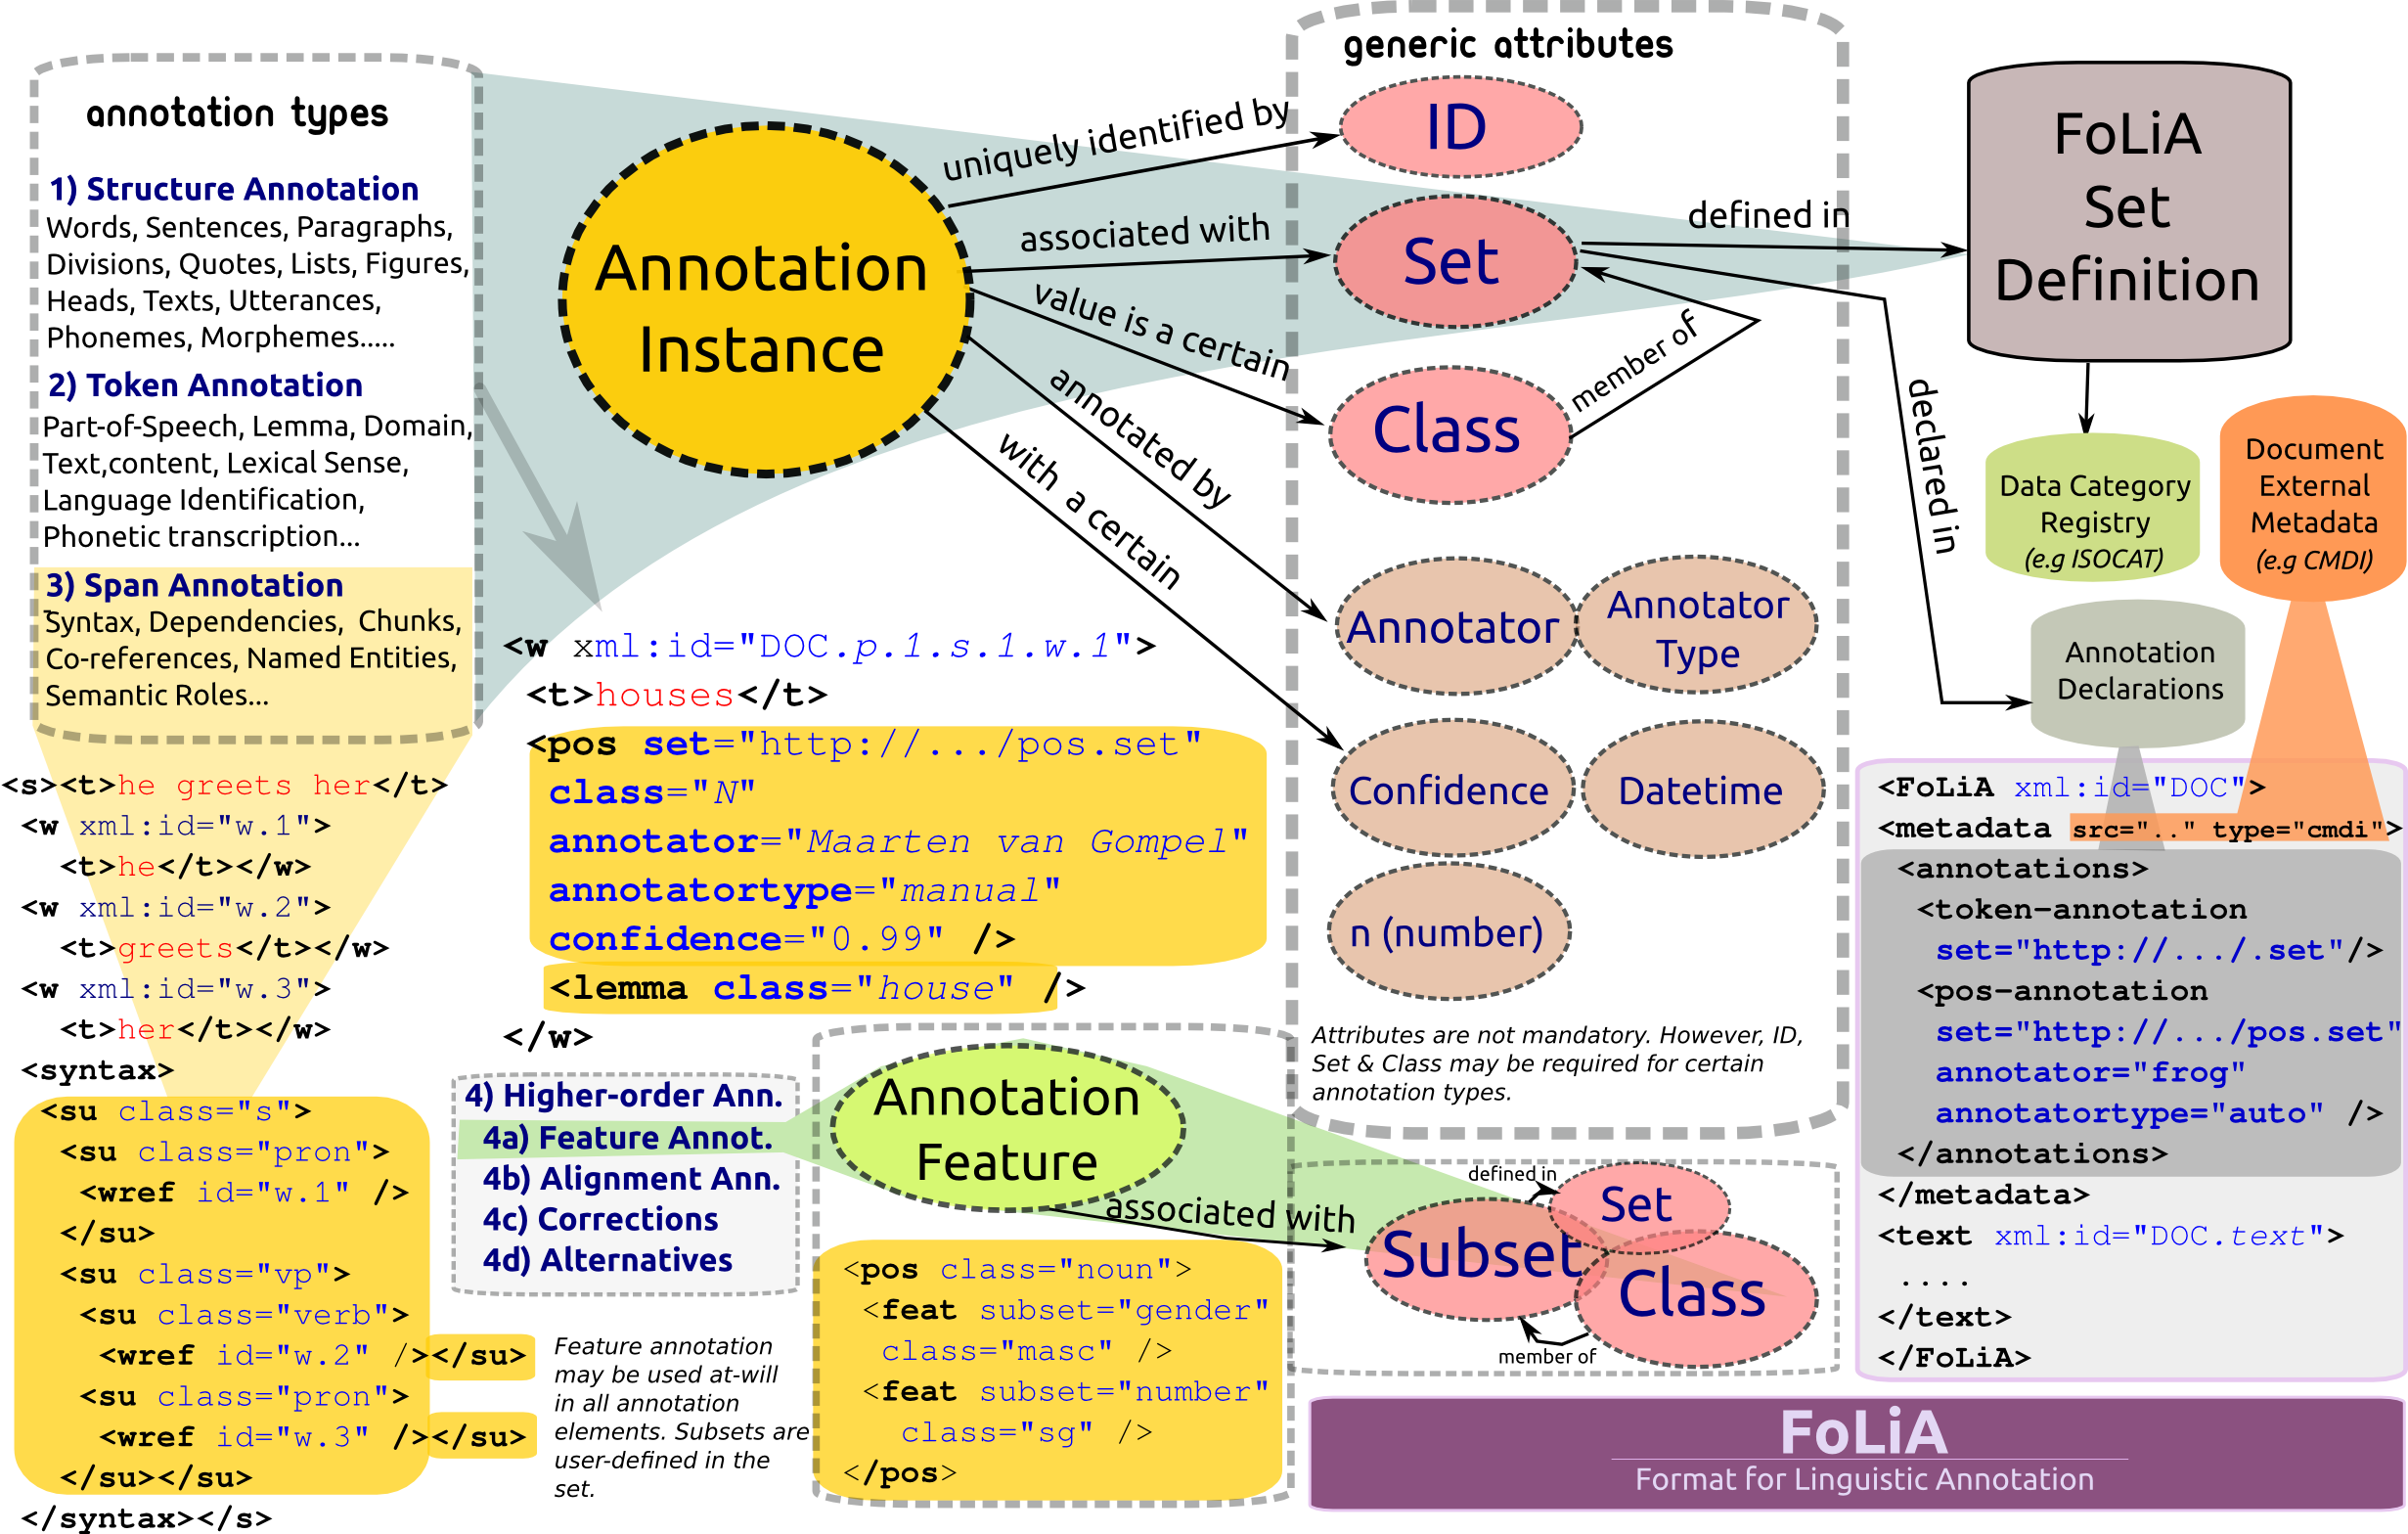
\includegraphics[width=145.0mm]{folia_paradigm.png}
\end{center}
\caption{The FoLiA Paradigm}
\label{fig:paradigm} 
\end{figure}

\subsection{Speech}
\label{sec:speechparadigm}

\status{Final since v0.12}{pynlpl,libfolia}

FoLiA is also suited for annotation of speech data. The following additional
FoLiA attributes are available for \emph{all} structure annotation elements in
a speech context: 

\begin{itemize}
  \item \texttt{src} -- \textbf{source} -- Points to a file or full URL of a sound or video file. This attribute is inheritable.
   
  \item \texttt{begintime} -- \textbf{begin time} --  A timestamp in
    \texttt{HH:MM:SS.MMM} format, indicating the begin time of the speech. If a
    sound clip is specified (\texttt{src}); the timestamp refers to a location
    in the soundclip. %(minus \texttt{srcoffset}).
    
  \item \texttt{endtime} -- \textbf{end time} --  A timestamp in
    \texttt{HH:MM:SS.MMM} format, indicating the end time of the speech. If a
    sound clip is specified (\texttt{src}); the timestamp refers to a location
    in the soundclip. %(minus \texttt{srcoffset}).
  
  %\item \texttt{srcoffset} -- \textbf{source offset} -- A timestamp in \texttt{HH:MM:SS.MMMM} format that is \emph{subtracted} from all \texttt{begintime}, and \texttt{endtime} designations within its scope, to find the position in the audio clip. This attribute enables the use of global timings in all begintime/endtime attributes, across different sound clips. Defaults to zero.
  
  \item \texttt{speaker} -- \textbf{speaker} -- A string identifying the
    speaker. This attribute is inheritable. Multiple speakers are not allowed,
    simply do not specify a speaker on a certain level if you are unable to
    link the speech to a specific (single) speaker.
\end{itemize}
 
Read more about speech annotation in Section~\ref{sec:speech}.

\section{Annotation Declaration}
\label{sec:declarations}

The annotation declaration is a mandatory part of the metadata that declares
all types of annotation and the sets that are present in the document.
Annotations are declared in the \texttt{annotations} block.

The follow example declares four annotation levels with fictitious sets and
several \emph{default attributes}:

\begin{lstlisting}[language=xml]
<annotations>
        <token-annotation 
          set="http://ilk.uvt.nl/folia/sets/ucto-tokconfig-nl" 
          annotator="ucto" annotatortype="auto" />
        <pos-annotation set="http://ilk.uvt.nl/folia/sets/CGN" 
          annotator="Frog" annotatortype="auto" />
        <lemma-annotation set="http://ilk.uvt.nl/folia/sets/lemmas-nl" 
          annotator="Frog" annotatortype="auto" />    
        <sense-annotation set="http://ilk.uvt.nl/folia/sets/Cornetto"
         annotator="SupWSD1" annotatortype="auto" />    
</annotations>
\end{lstlisting}

The set attribute is mandatory\footnote{Technically, it can be omitted, but
then the set defaults to ``undefined''. This is allowed for flexibility and
less explicit usage of FoLiA in limited settings, but not recommended!} and
refers to a URL of a FoLiA Set Definition file (see
Chapter~\ref{chapter:setdefinitions}). In the above example, the set URLs are
mostly fictitious. Throughout the documentation, we will either be using the dummy
value \texttt{http://url/to/your/set} for sets, or we will point to an actual
set definition, in which case you need to be aware this is merely and example
or suggestion which you are never obliged to use. You can always point to your
own sets.

A Set Definition specifies exactly what classes are allowed in the set. It for example
specifies exactly what Part-of-speech tags exist. This information is necessary
to validate the document completely at its deepest level. If the sets point
to URLs that do not exist or are not URLs at all, warnings will be issued.
Validation can still proceed but with the notable exception of deep validation
of these sets.

Though we recommend using and creating actual sets. FoLiA itself is rather
agnostic about their existence for most purposes. For deep validation, proper
formalisation, and for certain applications they may be required; but as long
as they serve as proper \emph{unique identifiers} you can work with
non-existing sets. In this case, simply do not use a URL but another arbitrary
identification string.

If multiple sets are used for the same annotation type, they each need a
separate declaration, as illustrated with the following fictitious sets:

\begin{lstlisting}[language=xml]
      <pos-annotation set="http://ilk.uvt.nl/folia/sets/CGN" 
        annotator="Frog" annotatortype="auto" />
      <pos-annotation set="http://ilk.uvt.nl/folia/sets/brown" />
\end{lstlisting}

If only one set is declared, then in the document itself you are allowed to
skip the set attribute on these specific annotation elements. The declared set
will automatically be the default. This is common practice as usually there is
only one set per annotation type.

The \texttt{annotator} and \texttt{annotatortype} attributes act as defaults
for the specific annotation type and set. Unlike \texttt{set}, you do
\emph{not} need, and it is in fact prohibited, to declare every possible
annotator here!

Annotator defaults can always be overridden at the specific annotation
elements. But declaring them allows for the annotation element to be less
verbosely expressed. Explicitly referring to a set and annotator for each
annotation element can be cumbersome and pointless in a document with a single
set and a single annotator for that particular type of annotation. Declarations
and defaults provide a nice way around this problem.


\section{Structure Annotation}
\label{sec:structureannotation}

\subsection{Basic Structural Elements}
\label{sec:basics}

Basic structural elements for textual documents occur within the \texttt{text} element. These are the most basic ones:

\begin{itemize}
\item \texttt{p} - Paragraph
\item \texttt{s} - Sentence
\item \texttt{w} - Word (token)
\end{itemize}

These are typically nested, the word elements cover the actual tokens. This is
the most basic level of annotation; tokenisation. Let's take a look at an
example where we have the following text:

\begin{verbatim}
This is a paragraph containing only one sentence.

This is the second paragraph. This one has two sentences.
\end{verbatim}

In FoLiA XML, this will appear as follows after tokenisation. Some parts have
been omitted for the sake of brevity:

\begin{lstlisting}[language=xml]
 <p xml:id="example.p.1">
    <s xml:id="example.p.1.s.1">        
        <w xml:id="example.p.1.s.1.w.1"><t>This</t></w>
        <w xml:id="example.p.1.s.1.w.2"><t>is</t></w>
        ...
        <w xml:id="example.p.1.s.1.w.8" space="no"><t>sentence</t></w>
        <w xml:id="example.p.1.s.1.w.9"><t>.</t></w>
    </s>
 </p>
 <p xml:id="example.p.2">
    <s xml:id="example.p.2.s.1">
        <w xml:id="example.p.2.s.1.w.1"><t>This</t></w>
        <w xml:id="example.p.2.s.1.w.2"><t>is</t></w>    
        ..
        <w xml:id="example.p.2.s.1.w.5" space="no"><t>paragraph</t></w>    
        <w xml:id="example.p.2.s.1.w.6"><t>.</t></w>    
    </s>
    <s xml:id="example.p.2.s.2">
        <w xml:id="example.p.2.s.2.w.1"><t>This</t></w>
        <w xml:id="example.p.2.s.2.w.2"><t>one</t></w>    
        ..
        <w xml:id="example.p.2.s.2.w.5" space="no"><t>sentences</t></w>    
        <w xml:id="example.p.2.s.2.w.6"><t>.</t></w>    
    </s>
 </p>
\end{lstlisting}

FoLiA is not just a format for holding tokenised text, although tokenisation is
a prerequisite for almost all kinds of annotation. However, FoLiA can also hold
untokenised text, on for example paragraph and/or sentence level:

\begin{lstlisting}[language=xml]
 <p xml:id="example.p.1">
    <s xml:id="example.p.1.s.1">        
        <t>This is a paragraph containing only one sentence.</t>
    </s>
 </p>
 <p xml:id="example.p.2">
    <s xml:id="example.p.2.s.1">     
        <t>This is the second paragraph.</t>
    </s>
    <s xml:id="example.p.2.s.2">     
        <t>This one has two sentences.</t>
    </s>    
 </p>
\end{lstlisting}

Higher level elements \emph{may} also contain a text element even when the
deeper elements do too. It is very important to realise that the
sentence/paragraph-level text element \emph{always} contains the text
\emph{prior} to tokenisation! Note also that the word element has an attribute
\texttt{space}, which defaults to yes, and indicates whether the word was
followed by a space in the \emph{untokenised} original. This allows for partial
reconstructibility of the sentence in its untokenised form. See
Section~\ref{sec:textcontent} for a more elaborate overview of this subject.

The following example shows the maximum amount of redundancy, with text
elements at every level.

\begin{lstlisting}[language=xml]
 <p xml:id="example.p.1">
    <t>This is a paragraph containing only one sentence.</t>
    <s xml:id="example.p.1.s.1">        
        <t>This is a paragraph containing only one sentence.</t>
        <w xml:id="example.p.1.s.1.w.1"><t>This</t></w>
        <w xml:id="example.p.1.s.1.w.2"><t>is</t></w>
        ...
        <w xml:id="example.sp.1.s.1.w.8" space="no"><t>sentence</t></w>
        <w xml:id="example.p.1.s.1.w.9"><t>.</t></w>
    </s>
 </p>
 <p xml:id="example.p.2">
    <t>This is the second paragraph. This one has two sentences.</t>
    <s xml:id="example.p.2.s.1">
        <t>This is the second paragraph.</t>
        <w xml:id="example.p.2.s.1.w.1"><t>This</t></w>
        <w xml:id="example.p.2.s.1.w.2"><t>is</t></w>    
        ..
        <w xml:id="example.p.2.s.1.w.5" space="no"><t>paragraph</t></w>    
        <w xml:id="example.p.2.s.1.w.6"><t>.</t></w>    
    </s>
    <s xml:id="example.p.2.s.2">
        <t>This one has two sentences.</t>
        <w xml:id="example.p.2.s.2.w.1"><t>This</t></w>
        <w xml:id="example.p.2.s.2.w.2"><t>one</t></w>    
        ..
        <w xml:id="example.p.2.s.2.w.5" space="no"><t>sentences</t></w>    
        <w xml:id="example.p.2.s.2.w.6"><t>.</t></w>    
    </s>
 </p>
\end{lstlisting}

If this kind of redundancy is used (it is not mandatory), you may optionally
point back to the text content of its parent by specifying the \texttt{offset}
attribute:

\begin{lstlisting}[language=xml]
 <p xml:id="example.p.1">
    <t>This is a paragraph containing only one sentence.</t>
    <s xml:id="example.p.1.s.1">        
        <t offset="0">This is a paragraph containing only one sentence.</t>
        <w xml:id="example.p.1.s.1.w.1">
        	<t offset="0">This</t>
        </w>
        <w xml:id="example.p.1.s.1.w.2">
        	<t offset="5">is</t>
        </w>
        ...
        <w xml:id="example.p.1.s.1.w.8" space="no">
        	<t offset="40">sentence</t>
        </w>
        <w xml:id="example.p.1.s.1.w.9">
        	<t offset="48">.</t>
        </w>
    </s>
 </p>
\end{lstlisting}

Matters can become more complicated as multiple text-content element of
different classes may be associated with an element, this will be discussed
later on in Section~\ref{sec:textcontent}.

Paragraph elements may be omitted if a document is described that does not
distinguish paragraphs but only sentences. Sentences, however, may never be
omitted; FoLiA documents can never consist of tokens only.

The content element \texttt{head} is reserved for headers and captions, it
behaves similarly to the paragraph element and holds sentences.


\subsection{Paragraphs, Sentences and Words}

Paragraphs, sentences and words (or tokens) are amongst the most elementary
structure elements. As we saw in a previous section, word elements (\texttt{w})
can take a class, pertaining to a certain set, at which point a declaration must
be present in the metadata:

\begin{declaration}
\begin{lstlisting}[language=xml]
<annotations>
 <token-annotation set="http://url/to/your/set" />
</annotations>
\end{lstlisting}
\end{declaration}

Being part of a set, this implies that tokens themselves \emph{may} be assigned
a class, as is for example done by the tokeniser \emph{ucto}:

\begin{lstlisting}[language=xml]
<s xml:id="example.p.1.s.1">
	<t>I see 2 children.</t>
    <w xml:id="example.p.1.s.1.w.1" class="WORD"><t>I</t></w>
    <w xml:id="example.p.1.s.1.w.2" class="WORD"><t>see</t></w>
    <w xml:id="example.p.1.s.1.w.3" class="NUMBER"><t>2</t></w>
    <w xml:id="example.p.1.s.1.w.4" class="WORD" space="no">
		<t>children</t>
    </w>
    <w xml:id="example.p.1.s.1.w.5" class="PUNCTUATION"><t>.</t></w>
</s>
\end{lstlisting}        

The same can be applied to paragraphs and sentences, which requires a
declaration of \texttt{paragraph-annotation} and \texttt{sentence-annotation}
respectively.

\begin{declaration}
\begin{lstlisting}[language=xml]
<annotations>
 <paragraph-annotation set="http://url/to/your/set" />
 <sentence-annotation set="http://url/to/your/set" />
</annotations>
\end{lstlisting}
\end{declaration}

\subsection{Divisions}

Within the \texttt{text} element, the structure element \texttt{div} can be
used to create divisions and subdivisions. Each division \emph{may} be of a
particular \emph{class} pertaining to a \emph{set} defining all possible
classes.

Divisions and other structural units are often numbered, think for example of
chapters and sections. The number, as it was in the source document, can be
encoded in the \texttt{n} attribute of the structure annotation element.

Look at the following example, showing a full FoLiA document with structured
divisions. The declared set is a fictitious example:

\begin{lstlisting}[language=xml]
<?xml version="1.0" encoding="utf-8"?>
<?xml-stylesheet type="text/xsl" 
 href="http://ilk.uvt.nl/FoLiA/FoLiA.xsl"?>
<FoLiA xmlns="http://ilk.uvt.nl/FoLiA"
  xmlns:xsi="http://www.w3.org/2001/XMLSchema-instance" 
  version="0.5"
  xml:id="example">
  <metadata>
      <annotations>
          <division-annotation 
           set="http://ilk.uvt.nl/folia/sets/divisions" />
      </annotations>    
  </metadata>
  <text xml:id="example.text">
     <div class="chapter" n="1">
        <head><t>Introduction</t></head>
        <div class="section" n="1">
            <div class="subsection" n="1.1">
                <t>In the beginning....</t>
            </div>
        </div>
        ...
     </div>
  </text>
</FoLiA>  
\end{lstlisting}

Divisions stem from D-Coi and are modified in FoLiA. These divisions are not
mandatory, but may be used to mark extra structure. D-Coi supports the elements
\texttt{div0}, \texttt{div1}, \texttt{div2}, etc.., but FoLiA only knows a
single \texttt{div} element, which can be nested at will and associated with
classes. Note that paragraphs, sentences and words have there own explicit
tags, as we saw earlier, divisions should never be used for marking these, only
larger structures can be divisions.

The \texttt{head} element may be used for the header of any division. It may
hold \texttt{s} and \texttt{w} elements (not \texttt{p}).

\begin{declaration}
\begin{lstlisting}[language=xml]
<annotations>
 <division-annotation set="https://raw.githubusercontent.com/proycon/folia/master/setdefinitions/divisions.foliaset.xml"
</annotations>
\end{lstlisting}
\end{declaration}

\subsection{Quotes}

\status{final since v0.3 (older versions are equal but lack declarations),
larger quotes allowing paragraphs and division since v0.11.3}{pynlpl, libfolia}

FoLiA supports quotes, using the \texttt{quote} element, to indicate that the
structural elements within are what
another person said or wrote:

\begin{lstlisting}[language=xml]
<quote xml:id="example.quote.1">
  <p xml:id="example.quote.1.p.1">
   <t>I have a dream that one day this nation will rise up and live out the
true meaning of its creed: "We hold these truths to be self-evident, that all
men are created equal."</t>
  </p>
  <p xml:id="example.quote.1.p.1">
   <t>I have a dream that one day on the red hills of Georgia, the sons of
former slaves and the sons of former slave owners will be able to sit down
together at the table of brotherhood.</t>
  </p>
</quote>
\end{lstlisting}

Quotes can be embedded in multiple levels, it may be a large block containing
itself divisions, paragraph or sentences, such as in the example above, or it
may be embedded in a sentence, in which case no divisions or paragraphs may
occur in the quote anymore.

One special case is the fact that sentences in sentences are allowed if they
are in a quote, this is demonstrated in the next example:

\begin{verbatim}
He said: ``I do not know . I think you are right. ", and left.
\end{verbatim}

A quote may consist of one or more sentences, but may also consist of mere tokens:

\begin{lstlisting}[language=xml]
 <s xml:id="example.p.1.s.1">
  <w xml:id="example.p.1.s.1.w.1" class="WORD"><t>He</t></w>
  <w xml:id="example.p.1.s.1.w.2" class="WORD"><t>said</t></w>
  <w xml:id="example.p.1.s.1.w.3" class="PUNCTUATION" space="no">
  	<t>:</t>
  </w>
  <w xml:id="example.p.1.s.1.w.4" class="PUNCTUATION" space="no">
  	<t>''</t>
  </w>
  <quote xml:id="example.p.1.s.1.quote.1">
    <s xml:id="example.p.1.s.1.quote.1.s.1">
       <w xml:id="example.p.1.s.1.w.5" class="WORD"><t>I</t></w>
       <w xml:id="example.p.1.s.1.w.6" class="WORD"><t>do</t></w>
       <w xml:id="example.p.1.s.1.w.7" class="WORD"><t>not</t></w>
       <w xml:id="example.p.1.s.1.w.8" class="WORD"><t>know</t></w>
       <w xml:id="example.p.1.s.1.w.9" class="PUNCTUATION" space="no">
       	<t>.</t>
       </w>
    </s>
    <s xml:id="example.p.1.s.1.quote.1.s.2">
       <w xml:id="example.p.1.s.1.w.10" class="WORD"><t>I</t></w>
       <w xml:id="example.p.1.s.1.w.11" class="WORD"><t>think</t></w>
       <w xml:id="example.p.1.s.1.w.12" class="WORD"><t>you</t></w>
       <w xml:id="example.p.1.s.1.w.13" class="WORD"><t>are</t></w>
       <w xml:id="example.p.1.s.1.w.14" class="WORD"><t>right</t></w>
    </s>
  </quote>
  <w xml:id="example.p.1.s.1.w.15" class="PUNCTUATION" space="no">
   <t>''</t>
  </w>
  <w xml:id="example.p.1.s.1.w.16" class="PUNCTUATION"><t>,</t></w>
  <w xml:id="example.p.1.s.1.w.17" class="WORD"><t>and</t></w>
  <w xml:id="example.p.1.s.1.w.18" class="WORD"><t>left</t></w>
  <w xml:id="example.p.1.s.1.w.19" class="PUNCTUATION" space="no">
  	<t>.</t>
  </w>
 </s>
\end{lstlisting}

\begin{nodeclaration}
Quotes are undeclarable elements
\end{nodeclaration}

\subsection{Gaps}

\status{final since v0.8 (older versions are equal but lack declarations)}{pynlpl, libfolia}

Sometimes there are parts of a document you want to skip and not annotate, but
include as is. For this purpose the \texttt{gap} element should be used. Gaps
may have a particular class indicating the kind of gap it is. Common omissions
are for example front-matter and back-matter.

The D-Coi format pre-defines the following ``reasons'' \cite{DCOI}:

\begin{itemize}
\item frontmatter
\item backmatter
\item illegible
\item other-language
\item cancelled
\item inaudible
\item sampling
\end{itemize}

Due to the flexible nature of FoLiA, we never predefine any classes whatsoever
and leave this up to whatever set is declared. The above gives a good
indication of what gaps can be used for though. 

The gap element may optionally take two elements:

\begin{enumerate}
\item \texttt{desc} - holding a substitute that may be shown to the user, describing what has been omitted.
\item \texttt{content} - The actual raw content of the omission, as it was without further annotations. This is an XML CDATA type element, excluding it from any kind of parsing.
\end{enumerate}


\begin{lstlisting}[language=xml]
  <text xml:id="example.text">
     <gap class="frontmatter" annotator="Maarten van Gompel">
        <desc>This is the cover of the book</desc>
        <content>
<![CDATA[        
    
            SHOW WHITE AND THE SEVEN DWARFS
            
            
                by the Brothers Grimm
                
                    first edition
                     
            
            Copyright(c) blah blah
]]>
        </content>
     </gap>
     <div class="chapter" n="1">
        <head><t>Introduction</t></head>
        <div class="section" n="1">
            <div class="subsection" n="1.1">
                <t>In the beginning....</t>
            </div>
        </div>
        ...
     </div>
  </text>
\end{lstlisting}

Gaps have to be declared:

\begin{declaration}
\begin{lstlisting}[language=xml]
<annotations>
 <gap-annotation set="https://raw.githubusercontent.com/proycon/folia/master/setdefinitions/gaps.foliaset.xml"
</annotations>
\end{lstlisting}
\end{declaration}



\subsection{Whitespace and Linebreaks}

\status{final}{pynlpl, libfolia}

Sometimes you may want to explicitly specify vertical whitespace or line
breaks. This can be done using respectively \texttt{whitespace} and
\texttt{br}. Both are simple structural elements that need not be declared.
Note that using \texttt{p} to denote paragraphs is always strongly preferred
over using \texttt{whitespace} to mark their boundaries!

\begin{lstlisting}[language=xml]
  <text xml:id="example.text">
    <s xml:id="example.s.1">
        <w xml:id="example.s.1.w.1">
        <br />
        <w xml:id="example.s.1.w.2">
        <w xml:id="example.s.1.w.3">
    </s>
    <whitespace />
    <s xml:id="example.s.2">
    </s>
  </text>
\end{lstlisting}

The difference between \texttt{br} and \texttt{whitespace} is that the former
specifies that only a linebreak was present, not forcing any vertical
whitespace, whilst the latter actually generates an empty space, which would
comparable to two successive \texttt{br} statements. Both elements can be used
inside divisions, paragraphs, headers, and sentences.

The \texttt{br} element has several optional attributes (since FoLiA v1.2) that can be set:

\begin{itemize}
    \item \texttt{newpage} Can be set to ``\texttt{yes}'' to indicate that the break is not just a linebreak, but also a pagebreak (defaults to ``no'')
    \item \texttt{pagenr} The number of the page after the break
    \item \texttt{linenr} The number of the line after the break
\end{itemize}

\begin{nodeclaration}
Whitespace and linebreaks are undeclarable elements.
\end{nodeclaration}

\subsection{Events}
\label{sec:events}

\status{final since v0.7}{pynlpl, libfolia}

Event structure,  though uncommon to regular written text, can be useful in
certain documents. Divisions, paragraphs, sentences, or even words can be
encapsulated in an event element to indicate they somehow form an event entity
of a particular class. This kind of structure annotation is especially useful
in dealing with written media such as chat logs, tweets, and internet fora, in
which chat turns, forum posts, and tweets can be demarcated as particular
events.

Below an example of a simple chat log, word tokens omitted for brevity:

\begin{lstlisting}[language=xml]
<event class="message" begindatetime="2011-12-15T19:01" 
 enddatetime="2011-12-15T19:05" actor="Jane Doe">
    <s>
        <t>Hello John.</t>
    </s>
    <s>
        <t>How are you doing?</t>
    </s>
</event>
<event class="message" begindatetime="2011-12-15T19:06"
 actor="John Doe">
    <s>
        <t>I am fine Jane, thanks.</t>
    </s>
</event>
\end{lstlisting}

The (optional) features \texttt{begindatetime} and \texttt{enddatetime} can be
used express the exact moment at which an event started or ended. Note that
this differs from the generic \texttt{datetime} attribute, which would describe
the time at which the annotation was recorded, rather than when the event took
place! Also, \texttt{begindatetime} and \texttt{enddatetime} are so-called
\emph{features} (see Section~\ref{sec:features})

For more fine-grained control over timed events, for example within sentences.
It is recommended to use the \texttt{timesegment} span annotation element
instead! This works in a very similar fashion but uses a stand-off annotation
layer. See Section~\ref{sec:timesegment}.

\begin{declaration}
\begin{lstlisting}[language=xml]
<annotations>
 <event-annotation
 set="https://raw.githubusercontent.com/proycon/folia/master/setdefinitions/events.foliaset.xml"
</annotations>
\end{lstlisting}
\end{declaration}

\subsection{Lists}

\status{final}{pynlpl, libfolia}

FoLiA, like D-Coi, allows lists to be explicitly marked as shown in the following example:

\begin{lstlisting}[language=xml]
 <head><t>My grocery list</t></head>
 <list xml:id="example.list.1">
   <item xml:id="example.list.1.item.1" n="A"><t>Apples</t></item>
   <item xml:id="example.list.1.item.2" n="B"><t>Pears</t></item>
 </list>
\end{lstlisting}

The item element may hold sentences \texttt{(s)} and words \texttt{(w)}. The
D-Coi format has a \texttt{label} element, this is deprecated in favour of the
\texttt{n} attribute in the item itself.

\begin{nodeclaration}
Lists are undeclarable elements.
\end{nodeclaration}

\subsection{Figures}

\status{final}{pynlpl, libfolia}

Even figures can be encoded in the FoLiA format, although the actual figure
itself can only be included as a mere reference to an external image file, but
including such a reference (\texttt{src} attribute) is optional.

\begin{lstlisting}[language=xml]
 <figure xml:id="example.figure.1" n="1" 
  src="/path/to/image/file">
   <desc>A textual description of the figure (Like ALT in HTML)</desc>
   <caption><t>The caption for the figure</t></caption>
 </figure>
\end{lstlisting}

The \texttt{caption} element may hold sentences
\texttt{(s)} and words \texttt{(w)}.

\begin{nodeclaration}
Figures are undeclarable elements.
\end{nodeclaration}

\subsection{Tables}

\status{since FoLiA 0.9.2}{pynlpl}

Support for simple tables is provided in a fashion similar to HTML and TEI. The
element \texttt{table} introduces a table, within its scope \texttt{row}
elements mark the various rows, \texttt{tablehead} marks the header of the
table and contains one or more rows. The rows themselves consist of
\texttt{cell} elements, which in turn may contain other structural elements
such as words, sentences or even entire paragraphs.

Consider the example below (not all elements have been assigned IDs for
brevity):

\begin{lstlisting}[language=xml]
<table xml:id="example.table.1">
  <tablehead>
    <row>
      <cell>
        <w xml:id="example.table.1.w.1"><t>Name</t></w>
      </cell>
      <cell>
        <w xml:id="example.table.1.w.2"><t>Affiliation</t></w>
      </cell>
    </row>
  </tablehead>
  <row>
    <cell>
      <w xml:id="example.table.1.w.3"><t>Maarten van Gompel</t></w>
    </cell>
    <cell>
      <w xml:id="example.table.1.w.4">
        <t>Radboud University Nijmegen</t>
      </w>
    </cell>
  </row>
  <row>
    <cell>
      <w xml:id="example.table.1.w.5"><t>Ko van der Sloot</t></w>
    </cell>
    <cell>
      <w xml:id="example.table.1.w.6"><t>Tilburg University</t></w>
    </cell>
  </row>
</table>
\end{lstlisting}

Tables, rows and cells can all be assigned classes, the declaration is as
follows:

\begin{declaration}
\begin{lstlisting}[language=xml]
<annotations>
 <table-annotation set="http://url/to/your/set" />
</annotations>
\end{lstlisting}
\end{declaration}

\subsection{Notes}

\status{since FoLiA 0.11.0}{pynlpl, libfolia}

The structure element \texttt{note} allows for notes to be included in FoLiA
documents. A footnote as well as a bibliographical reference is an example of a
note. The notes form an integral part of the text. For notes that are merely
descriptive comments on the texts or its annotations, rather than a part of it,
consider using \texttt{desc} instead. Notes themselves can contain all the
usual forms of annotations.

The place of a note in the text is where it will appear. References to the note
are made using a specific tag, \texttt{ref}, discussed in the next section.

\begin{lstlisting}[language=xml]
  <s><t>blah blah blah</t></s>
  <note xml:id="mynote" class="footnote">
    <s xml:id="mynote.s.1"><t>See our website!</t></s>
  </note>
</text>
\end{lstlisting}

Notes are also suited for building a bibliography:

\begin{lstlisting}[language=xml]
  <note xml:id="bib" class="bibref">
    <t>Maarten van Gompel (2014). FoLiA: Format for Linguistic Annotation.
Documentation. Language and Speech Technology Technical Report Series 14-01.
Radboud University Nijmegen</t>
  </note>
\end{lstlisting}

Whereas this section just presented the notes themselve, the next section will
discuss out to point to notes from within the text.

\begin{declaration}
\begin{lstlisting}[language=xml]
<annotations>
 <note-annotation
 set="https://raw.githubusercontent.com/proycon/folia/master/setdefinitions/notes.foliaset.xml"
</annotations>
\end{lstlisting}
\end{declaration}

\subsection{Structure References}
\label{sec:references}

\status{since FoLiA 0.11.0, support for external references since v1.2}{pynlpl, libfolia}

In the previous section we discussed notes, in this section we show that you
can make references to these notes using the \texttt{ref} element, this is a
structure element with an extra higher-order annotation function:

\begin{lstlisting}[language=xml]
<s>
  <t>We demonstrated this earlier.</t>
  <ref id="mynote" />
</s>
\end{lstlisting}

Another example in tokenised data, and now we add the \emph{optional} \texttt{type}
attribute, which holds the type of the FoLiA element that is referred to:

\begin{lstlisting}[language=xml]
<s>
  <w><t>We</t></w>
  <w><t>demonstrated</t></w>
  <w><t>this</t></w>
  <w><t>earlier</t></w>
  <w><t>.</t></w>
  <ref id="mynote" type="note" />
</s>
\end{lstlisting}

You can optionally make explicit the symbol used for the reference. When no
textual content is provided, whatever program renders the FoLiA document may assign its own
numbering or symbol.

\begin{lstlisting}[language=xml]
<s>
  <t>We demonstrated this earlier.</t>
  <ref id="mynote" type="note"><t>1</t></ref>
</s>
\end{lstlisting}

This is often needed for bibliographical references:

\begin{lstlisting}[language=xml]
<s>
  <t>We demonstrated this earlier.</t>
  <ref id="bib.1" type="note"><t>(van Gompel et al, 2014)</t></ref>
</s>
\end{lstlisting}

As a structure element, the \texttt{ref} element may contain other structure
elements such as words (\texttt{w}) or even sentences (\texttt{s}) or
paragraphs (\texttt{p}), which can in turn contain further linguistic
annotations.

Although we framed this section in the context of notes, the \texttt{ref} element is
more general and can be used whereever you need to explicitly refer to other \emph{structure
elements}. Common targets are figures, tables, divisions (sections, chapters,
etc). 

Being a structure element, the note reference itself may carry an ID as well.
Note that the ID attribute without the xml namespace always indicates a reference 
in FoLiA:

\begin{lstlisting}[language=xml]
<s><t>We demonstrated this earlier.</t></s>
<ref xml:id="myreference" id="mynote" />
\end{lstlisting}

The difference between the reference element and the higher-order alignments
(Section~\ref{sec:alignments}) needs to be clearly understood. Alignments lay
relations between annotations of any kind and thus pertain strongly to
linguistic annotation, whereas this reference element is a structural element
that is explicitly shown in the text and draws a reference that is explicitly
reflected in the text.

External references can also be made with the \texttt{ref} element, which
effectively makes it a valid tool for \emph{hyperlinking}. This is
done by setting the \texttt{xlink:href} to point to the external resource and
by setting the \texttt{format} attribute to the format of the external
resource. The format is understood to be a MIME type and its value defaults to
\texttt{text/folia+xml}. When an external reference is made, the \texttt{id}
attribute is optional and points to an element inside the external resource.

\begin{lstlisting}[language=xml]
<s>
  <w><t>We</t></w>
  <w><t>demonstrated</t></w>
  <w><t>this</t></w>
  <ref xlink:href="http://somewhere" xlink:type="simple" 
    format="text/html" id="section2">
    <w><t>here</t></w>
  </ref>
  <w><t>.</t></w>
</s>
\end{lstlisting}

This method of hyperlinking can be contrasted to the one described in
section~\ref{sec:hyperlinks}. These references offer a highly semantic way of
hyperlinking, whereas the other method is more of a text-markup or stylistic
nature.

\begin{nodeclaration}
The reference element itself is not declarable and takes no classes.
\end{nodeclaration}

\subsection{Parts}

\status{since FoLiA 0.11.2}{pynlpl, libfolia}

The structure element \texttt{part} is a fairly abstract structure element that
should only be used when a more specific structure element is not available. Most
notably, the part element should never be used for representation of morphemes
or phonemes! 

Part can be used to divide a larger structure element, such as a division, or a
paragraph into arbitrary subparts. 

\begin{lstlisting}[language=xml]
<p>
  <part xml:id="p.1.part.1">
    <t>First part of the paragraph.</t>
  </part>
  <part xml:id="p.2.part.2">
    <t>Last part of the paragraph.</t>
  </part>
</p>
\end{lstlisting}


The part element may seem alike to the division element, but divisions are used
for text blocks larger than a paragraph, typically correspondings to chapters,
sections or subsections and often carrying a \texttt{head} element. Do not use
parts for these structures.

The part element, on the other hand, is more abstract and plays a role on
a deeper level. It can be embedded within paragraphs, sentences, and most other
structure elements, even words, though we have to again emphasize it should not
be used for morphology, there are other solutions for that!

Contact the FoLiA authors if you find yourself using part and you feel a
more specific FoLiA element is missing.

\begin{declaration}
\begin{lstlisting}[language=xml]
<annotations>
 <part-annotation set="http://url/to/your/set" />
</annotations>
\end{lstlisting}
\end{declaration}

\subsection{Entries, definitions \& examples}
\label{sec:definitions}

\status{FoLiA 0.12}{pynlpl}

FoLiA has a set of structure element that can be used to represent
collections such as glossaries, dictionaries, thesauri, and wordnets.

These have in common that they consist of a set of entries, represented in
FoLiA by the \texttt{entry} element, and each entry is identified by one or
more terms, represented by the \texttt{term} element within an entry.

Terms need not be words, but a wide variety of structural elements can be used
as the term. Within the entry, these terms can subsequently be associated with
one or more definitions, using the \texttt{def} element, or with examples,
using the \texttt{ex} element. 

The \texttt{term}, \texttt{def} and \texttt{ex} elements can all take sets and
classes, and thus need to be declared. The \texttt{entry} elements themselves
are simple containers and need no declaration. Entries can contain multiple
terms if they are deemed dependent or related, such as in case of morphological
variants such as verb conjugations and declensions. The elements \texttt{term}
and \texttt{def} can only be used within an \texttt{entry}. The \texttt{ex}
element, however, can also be used standalone in different contexts.

In FoLiA, linguistic annotations are associated with the structure element
within the term itself. This is where a glossary can for instance obtain
part-of-speech or lexical semantic sense information, to name just a few
examples.

Below you see an example of a glossary entry, the sense set used comes from WordNet. The other sets are fictitious.

\begin{lstlisting}[language=xml]
<entry xml:id="entry.1">
 <term xml:id="entry.1.term.1">
  <w xml:id="entry.1.term.1.w.1">
    <t>house</t>
    <pos class="n">
      <feat subset="number" class="sing" />
    </pos>
    <lemma class="house" />
    <sense class="house\%1:06:00::">
  </w>
 </term>
 <term xml:id="entry.1.term.2">
  <w xml:id="entry.1.term.2.w.1">
    <t>houses/t>
    <pos class="n">
      <feat subset="number" class="plural" />
    </pos>
    <lemma class="house" />
    <sense class="house\%1:06:00::">
  </w>
 </term>
 <def xml:id="entry.1.def.1" class="sensedescription">
  <p xml:id="entry.1.def.1.p.1">
    <t>A dwelling, place of residence</t>
  </p>
 </def>
 <ex>
  <s xml:id="entry.1.ex.1.s.1> 
    <t>My house was constructed ten years ago.</t>
  </s>
 </ex>
</entry>
\end{lstlisting}

Other semantic senses would be represented as separate entries.

The definitions (\texttt{def}) are a generic element that can be used for
multiple types of definition. As always, the set is not predefined and purely
fictitious in our examples, giving the user flexibility. Definitions are for
instance suited for dictionaries:

\begin{lstlisting}[language=xml]
<entry xml:id="entry.1">
 <term xml:id="entry.1.term.1">
  <w xml:id="entry.1.term.1.w.1">
    <t>house</t>
    <pos set="englishpos" class="n">
      <feat subset="number" class="sing" />
    </pos>
    <lemma set="englishlemma" class="house" />
    <sense set="englishsense" class="house\%1:06:00::">
  </w>
 </term>
 <def xml:id="entry.1.def.1" class="translation-es">
  <w xml:id="entry.1.def.1.w.1">
    <t>casa</t>
    <pos set="spanishpos"  class="n">
      <feat subset="number" class="sing" />
    </pos>
    <lemma set="spanishlemma" class="casa" />
  </w>
 </def>
</entry>
\end{lstlisting}

Or for etymological definitions:

\begin{lstlisting}[language=xml]
 <def xml:id="entry.1.def.2" class="etymology">
  <p xml:id="entry.1.def.2.p.1">
   <t>Old English hus "dwelling, shelter, house," from Proto-Germanic *husan
 (cognates: Old Norse, Old Frisian hus, Dutch huis, German Haus), of unknown
 origin, perhaps connected to the root of hide (v.) [OED]. In Gothic only in
 gudhus "temple," literally "god-house;" the usual word for "house" in Gothic
 being razn.  </t>
  </p>
 </def>
\end{lstlisting}

To draw relations between entries and the terms therein, such as for example
for a wordnet, use FoLiA's \emph{alignments} (see
section~\ref{sec:alignments}).

The following two samples illustrate a dictionary distributed over multiple
FoLiA files, using alignments to link the two:

English part, \texttt{doc-english.xml}:

\begin{lstlisting}[language=xml]
<entry xml:id="en-entry.1">
 <term xml:id="en-entry.1.term.1">
  <w xml:id="en-entry.1.term.1.w.1">
    <t>house</t>
    <pos set="englishpos" class="n">
      <feat subset="number" class="sing" />
    </pos>
    <lemma set="englishlemma" class="house" />
    <sense set="englishsense" class="house\%1:06:00::">
  </w>
 </term>
 <alignment class="translation-es" xlink:href="doc-spanish.xml" 
    xlink:type="simple">
      <aref id="es-entry.1" type="entry" />
 </alignment>
</entry>
\end{lstlisting}

Spanish part, \texttt{doc-spanish.xml}:

\begin{lstlisting}[language=xml]
<entry xml:id="es-entry.1">
 <term xml:id="es-entry.1.def.1" class="translation-es">
  <w xml:id="entry.1.def.1.w.1">
    <t>casa</t>
    <pos set="spanishpos"  class="n">
      <feat subset="number" class="sing" />
    </pos>
    <lemma set="spanishlemma" class="casa" />
  </w>
 </term>
 <alignment class="translation-en" xlink:href="doc-english.xml" 
    xlink:type="simple">
      <aref id="en-entry.1" type="entry" />
 </alignment>
</entry>
\end{lstlisting}


For simple multilingual documents, explicit alignments may be too much hassle,
see Section~\ref{sec:translations} for a simpler methods based on convention.


\begin{declaration}
\begin{lstlisting}[language=xml]
<annotations>
 <term-annotation set="http://url/to/your/set" />
 <definition-annotation set="http://url/to/your/set" />
 <example-annotation set="http://url/to/your/set" />
</annotations>
\end{lstlisting}
\end{declaration}




\section{Token Annotation}
\label{sec:tokenannotation}

Token annotations are annotations that are placed within the structural
elements, often words/tokens (\texttt{w}) (hence the name), but also other
structure elements, in which case we speak of \emph{extended token annotation}. 

All token annotation elements may take all of the generic attributes described
in  Section~\ref{sec:paradigm}; this has to be kept in mind when reading this
section. Moreover, all token annotations depend on the document being
tokenised, i.e. there being \texttt{w} elements.

\subsection{Part-of-Speech Annotation}

\status{final}{pynlpl, libfolia}

Part-of-Speech annotation allows the annotation of lexical categories using the
\texttt{pos} element. The following example illustrates a simple Part-of-speech
annotation for the word ``boot'':

\begin{lstlisting}[language=xml]
<w xml:id="example.p.1.s.1.w.2">
    <t>boot</t>
    <pos class="N" />
</w>
\end{lstlisting}

Lexical annotation can take more complex forms than assignment of a single
part-of-speech tag. There may for example be numerous features associated with
the part-of-speech tag, such as gender, number, case, tense, mood, etc... FoLiA
introduces a special paradigm for dealing with such features. We will look into
this later, in Section~\ref{sec:higherorder}. 

Whenever part-of-speech annotations are used, they should be declared in the
\texttt{annotations} block as follows. The set you use may differ and all
further attributes are optional and are used to set defaults. In the
declaration example here it is as if the annotations were made by the software
\emph{Frog}, but you will want to use your own. 

\begin{declaration}
\begin{lstlisting}[language=xml]
<annotations>
 <pos-annotation set="http://url/to/your/set" />
</annotations>
\end{lstlisting}
\end{declaration}

As mentioned earlier, the declaration only sets defaults for annotator and
annotatortype. They can be overridden in the \texttt{pos} element itself (or
any other token annotation element for that matter).

\subsection{Lemma Annotation}

\status{final}{pynlpl, libfolia}

In the FoLiA paradigm, lemmas are perceived as classes within the (possibly
open) set of all possible lemmas. Their annotation proceeds as follows:

\begin{lstlisting}[language=xml]
<w xml:id="example.p.1.s.1.w.2">
    <t>boot</t>
    <lemma class="boot" />
</w>
\end{lstlisting}


\begin{declaration}
\begin{lstlisting}[language=xml]
<annotations>
 <lemma-annotation set="http://url/to/your/set" />
</annotations>
\end{lstlisting}
\end{declaration}

%\subsection{Phonetic Annotation}

%\status{final since v0.3}{pynlpl, libfolia}

%Phonetic annotations can be included as follows. Similarly to lemmas, they may often refer to a set with possibly open classes.

%\begin{lstlisting}[language=xml]
%<w xml:id="example.p.1.s.1.w.2">
 %   <t>boot</t>
 %   <phon-annotation set="http://ilk.uvt.nl/folia/sets/ipa" 
 %   class="bu:t" />
%</w>
%\end{lstlisting}

%This is an extended token annotation element that can also be used directly on a sentence or paragraph level.

%And the example declaration:

%\begin{lstlisting}[language=xml]
%<annotations>
    %<token-annotation set="http://ilk.uvt.nl/folia/sets/ucto-tokconfig-nl" 
     %annotator="ucto" annotatortype="auto" />
    %<phon-annotation set="http://ilk.uvt.nl/folia/sets/ipa" />
%</annotations>
%\end{lstlisting}

\subsection{Language Identification Annotation}

\status{final since v0.8.1}{pynlpl, libfolia}

Language identification is used to identify a certain element as being in a
certain language. In FoLiA, the \texttt{lang} element is used to identify
language:

\begin{lstlisting}[language=xml]
<w xml:id="example.p.1.s.1.w.2">
    <t>boot</t>
	<lang class="eng" />
</w>
\end{lstlisting}

This is an extended token annotation element that can also be used directly on
other levels, such as a sentence, paragraph, division, or text level

\begin{declaration}
\begin{lstlisting}[language=xml]
<annotations>
 <lang-annotation set="http://url/to/your/set" />
</annotations>
\end{lstlisting}
\end{declaration}

\subsection{Lexical Semantic Sense Annotation}

\status{final}{pynlpl,libfolia}

In semantic sense annotation, the classes in most sets will be a kind of
lexical unit ID. In systems that make a distinction between lexical units and
synonym sets (synsets), the synset attribute is available for notation of the
latter. In systems with only synsets and no other primary form of lexical unit,
the class can simply be set to the synset.

A human readable description for the \emph{sense} element, ``beeldhouwwerk'',
could be placed inside a \texttt{desc} element, but this is optional.

\begin{lstlisting}[language=xml]
<w xml:id="example.p.1.s.1.w.2">
    <t>beeld</t>
    <sense class="r_n-6220" synset="d_n-32683">
    	<desc>beeldhouwwerk</desc>
    </sense>
</w>
\end{lstlisting}

The example declaration is as follows:

\begin{declaration}
\begin{lstlisting}[language=xml]
<annotations>
 <sense-annotation set="http://url/to/your/set" />
</annotations>
\end{lstlisting}
\end{declaration}

\subsection{Domain Tags}

\status{final}{pynlpl,libfolia}

Domain annotation is used to associate a certain domain with a structural
element. This is an extended token annotation element, which means it can also
be used directly in any of the content elements, such as sentence (\texttt{s})
and  paragraph (\texttt{p}). It can even be used in the \texttt{text} element
itself. Example:

\begin{lstlisting}[language=xml]
<w xml:id="example.p.1.s.1.w.2">
    <t>boot</t>
    <domain class="nautical" />
</w>
\end{lstlisting}

The declaration (the actual set is fictitious):

\begin{declaration}
\begin{lstlisting}[language=xml]
<annotations>
 <domain-annotation set="http://url/to/your/set" />
</annotations>
\end{lstlisting}
\end{declaration}

\subsection{Subjectivity/Sentiment Analysis}

\status{final}{pynlpl,libfolia}

Subjectivity annotation is used to associate a certain subjective quality with
a structural element. It is used for sentiment analysis and opinion analysis.
Example:

\begin{lstlisting}[language=xml]
<w xml:id="example.p.1.s.1.w.2">
    <t>hate</t>
    <subjectivity class="negative" />
</w>
\end{lstlisting}

The declaration (the actual set is fictitious):

\begin{declaration}
\begin{lstlisting}[language=xml]
<annotations>
 <subjectivity-annotation set="http://url/to/your/set" />
</annotations>
\end{lstlisting}
\end{declaration}



\section{Span Annotation}
\label{sec:spanannotation}

Not all annotations can be realised as token annotations. Some typically span
multiple tokens. For these we introduce a kind of offset notation in separate
\emph{annotation layers}.  Within these layers, references are made to all of
the word tokens spanned using the \texttt{wref} element. Each annotation layer
is specific to a kind of span annotation and associated with a set, for which a
declaration should be present in the metadata section of the document.  The
annotation layers are generally embedded within the structure element that also
contains all the words that are referenced. Often this corresponds to the
sentence level. Any other higher level is fine too, though. Layers are always
embedded \emph{after} the word tokens or other structural elements.

Depending on the type of span annotation, it is possible that the element may
be nested. This is for example the case for syntactic annotation, where the
nesting of syntactic units allows the building of syntax trees. Other span
annotation elements of a more complex nature may require other span annotation
elements within them, these latter span annotation elements are then known as
\emph{span roles}. Span roles can only be used in
the scope of a certain span annotation element, not standalone, and therefore
do not have their own dedicated layer.


%The layer elements themselves may also take the \texttt{set}, \texttt{annotator}, \texttt{annotatortype}, or \texttt{confidence} attributes. Which introduces the defaults for all the span annotations under it. They in turn may of course always chose to override this. %DISABLED FOR NOW, LIBRARIES DON't IMPLEMENT THIS YET

\subsection{Entities}

\status{final}{pynlpl,libfolia}

The \texttt{entities} layer offers a generic solution to encode various types
of entities or multi-word expressions, including but not limited to named
entities. The set used determines the precise semantics behind the entities.

Below is an example of named entity annotation of a full sentence in which one
name is tagged. It is recommended for each entity to have a unique identifier.

\begin{lstlisting}[language=xml]
<s xml:id="example.p.1.s.1">
  <t>The Dalai Lama greeted him.</t>
  <w xml:id="example.p.1.s.1.w.1"><t>The</t></w>
  <w xml:id="example.p.1.s.1.w.2"><t>Dalai</t></w>
  <w xml:id="example.p.1.s.1.w.3"><t>Lama</t></w>
  <w xml:id="example.p.1.s.1.w.4"><t>greeted</t></w>
  <w xml:id="example.p.1.s.1.w.5"><t>him</t></w>
  <w xml:id="example.p.1.s.1.w.6"><t>.</t></w>
  <entities>
    <entity xml:id="example.p.1.s.1.entity.1" class="per">
        <wref id="example.p.1.s.1.w.2" t="Dalai" />
        <wref id="example.p.1.s.1.w.3" t="Lama" />
    </entity>
  </entities>
</s>
\end{lstlisting}

Note that elements that are not part of any span annotation need never be
included in the layer. The \texttt{wref} element takes an \emph{optional}
\texttt{t} attribute which contains a copy of the text of the word pointed at.
This is to facilitate human readability and prevent the need for resolving
words for simple applications in which only the textual content is of interest.

\begin{declaration}
\begin{lstlisting}[language=xml]
<annotations>
 <entity-annotation
 set="https://raw.githubusercontent.com/proycon/folia/master/setdefinitions/namedentities.foliaset.xml"
</annotations>
\end{lstlisting}
\end{declaration}

\subsection{Syntax}

\status{final}{pynlpl,libfolia}

A very typical form of span annotation is syntax annotation. This is done
within the \texttt{syntax} layer and introduces a nested hierarchy of syntactic
unit (\texttt{su}) elements. It is recommended for each syntactic unit to have
a unique identifier:

\begin{lstlisting}[language=xml]
<s xml:id="example.p.1.s.1">
  <t>The Dalai Lama greeted him.</t>
  <w xml:id="example.p.1.s.1.w.1"><t>The</t></w>
  <w xml:id="example.p.1.s.1.w.2"><t>Dalai</t></w>
  <w xml:id="example.p.1.s.1.w.3"><t>Lama</t></w>
  <w xml:id="example.p.1.s.1.w.4"><t>greeted</t></w>
  <w xml:id="example.p.1.s.1.w.5"><t>him</t></w>
  <w xml:id="example.p.1.s.1.w.6"><t>.</t></w>
  <syntax>
    <su xml:id="example.p.1.s.1.su.1" class="s">     
      <su xml:id="example.p.1.s.1.su.1_1" class="np">
          <su xml:id="example.p.1.s.1.su.1_1_1" class="det">
             <wref id="example.p.1.s.1.w.1" t="The" />       
          </su>
          <su xml:id="example.p.1.s.1.su.1_1_2" class="pn">
             <wref id="example.p.1.s.1.w.2" t="Dalai" />
             <wref id="example.p.1.s.1.w.3" t="Lama" />        
          </su>         
       </su>
     </su>
     <su xml:id="example.p.1.s.1.su.1_2" class="vp"> 
        <su xml:id="example.p.1.s.1.su.1_1_1" class="v">
            <wref id="example.p.1.s.1.w.4" t="greeted" />       
        </su>
        <su xml:id="example.p.1.s.1.su.1_1_2" class="pron">
          <wref id="example.p.1.s.1.w.5" t="him" />       
        </su>
     </su>    
    </su>
  </syntax>
</s>
\end{lstlisting}

As is prescribed by the FoLiA paradigm the classes always depend on the set
used. You can use whatever system of syntactic annotation you desire. Moreover,
any of the \texttt{su} elements can have the common attributes
\texttt{annotator}, \texttt{annotatortype} and \texttt{confidence}.

The above example illustrates a fairly simple syntactic parse. Dependency
parses are possible too. Dependencies are listed separate from the syntax in an
extra annotation layer, see Section~\ref{sec:deprel}.

\begin{declaration}
\begin{lstlisting}[language=xml]
<annotations>
 <syntax-annotation set="http://path/to/your/set"
</annotations>
\end{lstlisting}
\end{declaration}

\subsection{Dependency Relations}
\label{sec:deprel}

\status{slightly revised in v0.8 (no ``su'' attribute on hd/dep)}{pynlpl,libfolia}

Dependency relations are relations between tokens, in most cases equal to
syntactic units. A dependency relation is often of a particular class and
consists of a single head component and a single dependent component. In the
sample ``He sees'', there is  syntactic dependency between the two words:
``sees'' is the head, and ``He'' is the dependant, and the relation class is
something like ``subject'', as the dependant is the subject of the head word.
Each dependency relation is explicitly noted in FoLiA.

The element \texttt{dependencies} introduces this annotation layer. Within it,
\texttt{dependency} elements describe all dependency pairs. 

In the example below, we show a Dutch sentence parsed with the Alpino Parser
\cite{ALPINO}. We show not only the dependency layer, but also the syntax layer
to which it is related. The \texttt{dependency} element always contains two
span roles: one head element (\texttt{hd}) and one dependent element
(\texttt{dep}). The words they cover are reiterated in the usual fashion, using
\texttt{wref}. For a better understanding, Figure~\ref{fig:depparse}
illustrates the syntactic parse with the dependency relations. Both span roles \texttt{hd}
and \texttt{dep} can optionally make extra reference to a syntactic unit (or
anything else for that matter) by means of the \texttt{aref} element. 

\begin{figure}[h]
\begin{center}
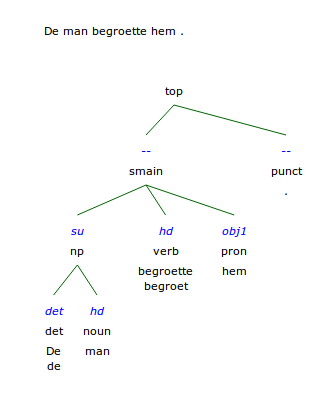
\includegraphics[width=60.0mm]{alpino.png}
\end{center}
\caption{Alpino dependency parse for the Dutch sentence ``De man begroette hem.''}
\label{fig:depparse} 
\end{figure}
\FloatBarrier

\begin{lstlisting}[language=xml]
<s xml:id="example.p.1.s.1">
  <t>De man begroette hem.</t>
  <w xml:id="example.p.1.s.1.w.1"><t>De</t></w>
  <w xml:id="example.p.1.s.1.w.2"><t>man</t></w>
  <w xml:id="example.p.1.s.1.w.3"><t>begroette</t></w>
  <w xml:id="example.p.1.s.1.w.4"><t>hem</t></w>
  <w xml:id="example.p.1.s.1.w.5"><t>.</t></w>
  <syntax>
    <su xml:id="example.p.1.s.1.su.1" class="top">     
        <su xml:id="example.p.1.s.1.su.1_1" class="smain">     
            <su xml:id="example.p.1.s.1.su.1_1_1" class="np">     
                <su xml:id="example.p.1.s.1.su.1_1_1_1" class="top">     
                    <wref id="example.p.1.s.1.w.1" t="De" />       
                </su>
                <su xml:id="example.p.1.s.1.su.1_1_1_2" class="top">     
                    <wref id="example.p.1.s.1.w.2" t="man" />
                </su> 
            </su>
            <su xml:id="example.p.1.s.1.su.1_1_2" class="verb">     
                <wref id="example.p.1.s.1.w.3" t="begroette" />   
            </su>
            <su xml:id="example.p.1.s.1.su.1_1_3" class="pron">     
                <wref id="example.p.1.s.1.w.4" t="hem" />   
            </su>
        </su>
        <su xml:id="example.p.1.s.1.su.1_2" class="punct">
            <wref id="example.p.1.s.1.w.5" t="." />               
        </su> 
    </su>
  </syntax>
  <dependencies>    
    <dependency xml:id="example.p.1.s.1.dependency.1" class="su">
        <hd>
            <wref id="example.p.1.s.1.w.3" t="begroette">
            <aref id="example.p.1.s.1.su.1_1_2" type="su">
        </hd>
        <dep>
            <wref id="example.p.1.s.1.w.2" t="man" />  
            <aref id="example.p.1.s.1.su.1_1_1" type="su">     
        </dep>
    </dependency>        
    <dependency xml:id="example.p.1.s.1.dependency.3" class="obj1">
        <hd>
            <wref id="example.p.1.s.1.w.3" t="begroette">
            <aref id="example.p.1.s.1.su.1_1_2" type="su">
        </hd>
        <dep>
            <wref id="example.p.1.s.1.w.4" t="hem" />   
            <aref id="example.p.1.s.1.su.1_1_3" type="su">
        </dep>
    </dependency>
    <dependency xml:id="example.p.1.s.1.dependency.2" class="det">
        <hd>           
           <wref id="example.p.1.s.1.w.2" t="man" />   
           <aref id="example.p.1.s.1.su.1_1_1_2" type="su">
        </hd>
        <dep>            
            <wref id="example.p.1.s.1.w.1" t="De" />   
            <aref id="example.p.1.s.1.su.1_1_1_1" type="su">
        </dep>
    </dependency>   
  </dependencies>
</s>
\end{lstlisting}


Note that in the first dependency relation, the dependant is just ``man''
rather than ``de man'' . That is, we point only to the head of dependants, the
full scope follows automatically when building the dependency tree.


\begin{declaration}
\begin{lstlisting}[language=xml]
<annotations>
 <syntax-annotation set="http://url/to/your/set" />
 <dependency-annotation set="http://url/to/your/set" />
</annotations>
\end{lstlisting}
\end{declaration}

\subsection{Chunking}

\status{final}{pynlpl,libfolia}

Unlike a full syntactic parse, chunking is not nested. The layer for this type
of linguistic annotation is predictably called \texttt{chunking}. The span
annotation element itself is \texttt{chunk}.

\begin{lstlisting}[language=xml]
<s xml:id="example.p.1.s.1">
  <t>The Dalai Lama greeted him.</t>
  <w xml:id="example.p.1.s.1.w.1"><t>The</t></w>
  <w xml:id="example.p.1.s.1.w.2"><t>Dalai</t></w>
  <w xml:id="example.p.1.s.1.w.3"><t>Lama</t></w>
  <w xml:id="example.p.1.s.1.w.4"><t>greeted</t></w>
  <w xml:id="example.p.1.s.1.w.5"><t>him</t></w>
  <w xml:id="example.p.1.s.1.w.6"><t>.</t></w>
  <chunking>
    <chunk xml:id="example.p.1.s.1.chunk.1">       
        <wref id="example.p.1.s.1.w.1" t="The" />       
        <wref id="example.p.1.s.1.w.2" t="Dalai" />       
        <wref id="example.p.1.s.1.w.3" t="Lama" />        
    </chunk>
    <chunk xml:id="example.p.1.s.1.chunk.2">       
        <wref id="example.p.1.s.1.w.4" t="greeted" />
    </chunk>
    <chunk xml:id="example.p.1.s.1.chunk.3">       
        <wref id="example.p.1.s.1.w.5" t="him" />
        <wref id="example.p.1.s.1.w.6" t="." />
    </chunk>    
  </chunking>
</s>
\end{lstlisting}


The declaration (the actual sets are fictitious):

\begin{declaration}
\begin{lstlisting}[language=xml]
<annotations>
 <chunking-annotation set="http://url/to/your/set" />
</annotations>
\end{lstlisting}
\end{declaration}

\subsection{Time Segmentation}
\label{sec:timesegment}

\status{final since v0.8, renamed in v0.9}{pynlpl,libfolia}

FoLiA supports time segmentation using the \texttt{timing} layer and the
\texttt{timesegment} span annotation element. This element is useful for
speech, but can also be used for event annotation. We already saw events as
structure annotation in Section~\ref{sec:events}, but for more fine-grained
control of timing information a span annotation element in an offset layer is
more suited. The following example illustrates the usage for event annotation:

\begin{lstlisting}[language=xml]
<s>
 <w xml:id="example.p.1.s.1.w.1"><t>I</t></w>
 <w xml:id="example.p.1.s.1.w.2"><t>think</t></w>
 <w xml:id="example.p.1.s.1.w.3"><t>I</t></w>
 <w xml:id="example.p.1.s.1.w.4"><t>have</t></w>
 <w xml:id="example.p.1.s.1.w.5"><t>to</t></w>
 <w xml:id="example.p.1.s.1.w.6"><t>go</t></w>
 <w xml:id="example.p.1.s.1.w.7"><t>.</t></w>
 <timing>
  <timesegment class="utterance" begindatetime="2011-12-15T19:01" 
   enddatetime="2011-12-15T19:03" actor="myself">
    <wref id="example.p.1.s.1.w.1" t="I" />
    <wref id="example.p.1.s.1.w.2" t="think" />
  </timesegment>
  <timesegment class="cough" begindatetime="2011-12-15T19:03" 
   enddatetime="2011-12-15T19:05" actor="myself">   
  </timesegment>
  <timesegment class="utterance" begindatetime="2011-12-15T19:05" 
   enddatetime="2011-12-15T19:06" actor="myself">
    <wref id="example.p.1.s.1.w.3" t="I" />
    <wref id="example.p.1.s.1.w.4" t="have" />
    <wref id="example.p.1.s.1.w.5" t="to" />
    <wref id="example.p.1.s.1.w.6" t="go" />
  </timesegment>
 </timing>
</s>
\end{lstlisting}


Time segments may also be nested. As always, the classes in the example are
set-defined rather than predefined by FoLiA. The predefined and optional
features \texttt{begindatetime} and \texttt{enddatetime} can be used express
the exact moment at which an event started or ended. These too are set-defined
so the format shown here is just an example.





If you are only interested in an annotation of events, and a coarser level of
annotation suffices, then use the structure annotation element \texttt{event}
instead. See Section~\ref{sec:events}.


\textbf{Note:} Time segments were known as "timed events" in FoLiA 0.8 and
below. They have been renamed to a more appropriate and more generic name. For
backward compatibility, libraries should implement \texttt{timedevent} as an
alias for \texttt{timesegment}, and \texttt{timedevent-annotation} as an alias
for \texttt{timesegment-annotation}.

\begin{declaration}
\begin{lstlisting}[language=xml]
<annotations>
 <timesegment-annotation set="http://url/to/your/set" />
</annotations>
\end{lstlisting}
\end{declaration}

\subsubsection{Time segmentation in a speech context}

\status{final since v0.10}{pynlpl,libfolia}

If used in a speech context, all the generic speech attributes become available
(See Section~\ref{sec:speech}). This introduces  \texttt{begintime} and
\texttt{endtime}, which are different from \texttt{begindatetime} and
\texttt{enddatetime} ! The generic attributes \texttt{begintime} and
\texttt{endtime} are not defined by the set, but specify a time location in
\texttt{HH:MM:SS.MMM} format which may refer to the location in an associated sound
file. Sound files are associated using the \texttt{src} attribute, which is
inherited by all lower elements, so we put it on the sentence here:

\begin{lstlisting}[language=xml]
<s src="ithinkihavetogo.mp3">
 <w xml:id="example.p.1.s.1.w.1"><t>I</t></w>
 <w xml:id="example.p.1.s.1.w.2"><t>think</t></w>
 <w xml:id="example.p.1.s.1.w.3"><t>I</t></w>
 <w xml:id="example.p.1.s.1.w.4"><t>have</t></w>
 <w xml:id="example.p.1.s.1.w.5"><t>to</t></w>
 <w xml:id="example.p.1.s.1.w.6"><t>go</t></w>
 <w xml:id="example.p.1.s.1.w.7"><t>.</t></w>
 <timing>
  <timesegment begintime="00:00:00.000" 
   endtime="00:00:00.250">
    <wref id="example.p.1.s.1.w.1" t="I" />
  </timesegment>
  <timesegment begintime="00:00:00.250" 
   endtime="00:00:00.500">
    <wref id="example.p.1.s.1.w.2" t="think" />
  </timesegment>
  <timesegment begintime="00:00:00.500" 
   endtime="00:00:00.750">
    <wref id="example.p.1.s.1.w.3" t="I" />
  </timesegment>
  <timesegment begintime="00:00:00.750" 
   endtime="00:00:01.000">
    <wref id="example.p.1.s.1.w.4" t="have" />
  </timesegment>
  <timesegment begintime="00:00:01.000" 
   endtime="00:00:01.250">
    <wref id="example.p.1.s.1.w.5" t="to" />
  </timesegment>
  <timesegment begintime="00:00:01.250" 
   endtime="00:00:01.500">
    <wref id="example.p.1.s.1.w.6" t="go" />
  </timesegment>
 </timing>
</s>
\end{lstlisting}

In a speech context, all structural elements may carry the generic attributes.
So the time segmentation in the previous example, though valid, is not the most
intuitive way of accomplishing this. Instead, time segmentation can better be
used when actual classes are assigned:

\begin{lstlisting}[language=xml]
<s src="ithinkihavetogo.mp3">
 <w xml:id="example.p.1.s.1.w.1"
  begintime="00:00:00.000" endtime="00:00:00.250"><t>I</t></w>
 <w xml:id="example.p.1.s.1.w.2"
  begintime="00:00:00.250" endtime="00:00:00.500"><t>think</t></w>
 <w xml:id="example.p.1.s.1.w.3" 
  begintime="00:00:00.500" endtime="00:00:00.750"><t>I</t></w>
 <w xml:id="example.p.1.s.1.w.4"
  begintime="00:00:00.750" endtime="00:00:01.000"><t>have</t></w>
 <w xml:id="example.p.1.s.1.w.5" 
  begintime="00:00:01.000" endtime="00:00:01.250"><t>to</t></w>
 <w xml:id="example.p.1.s.1.w.6" 
  begintime="00:00:01.250" endtime="00:00:01.500"><t>go</t></w>
 <w xml:id="example.p.1.s.1.w.7"><t>.</t></w>
 <timing>
	<timesegment class="emphasised">
		<wref id="example.p.1.s.1.w.3" />
		<wref id="example.p.1.s.1.w.4" />
		<wref id="example.p.1.s.1.w.5" />
		<wref id="example.p.1.s.1.w.6" />
	</timesegment>
 </timing>
</s>
\end{lstlisting}

This usage, and the freedom FoLiA sets offer, opens up possibilities for a wide
variety of time-segmented annotations. Moreover, the wref element does not
necessarily point at words, but it may also point at phonemes. This will be
introduced in Section~\ref{sec:phonemes}.

 
\subsection{Semantic Roles}

\status{new in 0.9}{pynlpl}

Semantic roles, or thematic roles, are implemented in FoLiA using the
span-annotation element \texttt{semrole}, within the annotation layer
\texttt{semroles}, usually embedded at sentence level.

\begin{lstlisting}[language=xml]
<s xml:id="example.p.1.s.1">
  <t>The Dalai Lama greeted him.</t>
  <w xml:id="example.p.1.s.1.w.1"><t>The</t></w>
  <w xml:id="example.p.1.s.1.w.2"><t>Dalai</t></w>
  <w xml:id="example.p.1.s.1.w.3"><t>Lama</t></w>
  <w xml:id="example.p.1.s.1.w.4"><t>greeted</t></w>
  <w xml:id="example.p.1.s.1.w.5"><t>him</t></w>
  <w xml:id="example.p.1.s.1.w.6"><t>.</t></w>
  <semroles>
	<semrole class="agent">
		<wref id="example.p.1.s.1.w.2" />
		<wref id="example.p.1.s.1.w.3" />
	</semrole>
	<semrole class="patient">
		<wref id="example.p.1.s.1.w.5" />
	</semrole>
  </semroles>
</s>
\end{lstlisting}

Semantic roles commonly correspond with syntactic units. Links between the two
can be expressed using FoLiA's facility for alignments (see also
Section~\ref{sec:alignments}), which were already seen in dependency relations
as well. The \texttt{aref} element may be used from within the \texttt{semrole}
element to link to a syntactic unit, or anything else for that matter. The
following example illustrates this:

\begin{lstlisting}[language=xml]
<s xml:id="example.p.1.s.1">
  <t>De man begroette hem.</t>
  <w xml:id="example.p.1.s.1.w.1"><t>De</t></w>
  <w xml:id="example.p.1.s.1.w.2"><t>man</t></w>
  <w xml:id="example.p.1.s.1.w.3"><t>begroette</t></w>
  <w xml:id="example.p.1.s.1.w.4"><t>hem</t></w>
  <w xml:id="example.p.1.s.1.w.5"><t>.</t></w>
  <syntax>
    <su xml:id="example.p.1.s.1.su.1" class="top">     
        <su xml:id="example.p.1.s.1.su.1_1" class="smain">     
            <su xml:id="example.p.1.s.1.su.1_1_1" class="np">     
                <su xml:id="example.p.1.s.1.su.1_1_1_1" class="top">     
                    <wref id="example.p.1.s.1.w.1" t="De" />       
                </su>
                <su xml:id="example.p.1.s.1.su.1_1_1_2" class="top">     
                    <wref id="example.p.1.s.1.w.2" t="man" />
                </su> 
            </su>
            <su xml:id="example.p.1.s.1.su.1_1_2" class="verb">     
                <wref id="example.p.1.s.1.w.3" t="begroette" />   
            </su>
            <su xml:id="example.p.1.s.1.su.1_1_3" class="pron">     
                <wref id="example.p.1.s.1.w.4" t="hem" />   
            </su>
        </su>
        <su xml:id="example.p.1.s.1.su.1_2" class="punct">
            <wref id="example.p.1.s.1.w.5" t="." />               
        </su> 
    </su>
  </syntax>
  <semroles>
	<semrole class="agent">
		<wref id="example.p.1.s.1.w.1" />
		<wref id="example.p.1.s.1.w.2" />
		<aref id="example.p.1.s.1.su.1_1_1" type="su">
	</semrole>
	<semrole class="patient">
		<wref id="example.p.1.s.1.w.4" />
		<aref id="example.p.1.s.1.su.1_1_3" type="su">
	</semrole>
  </semroles>
</s>
\end{lstlisting}

The \texttt{hd} element can optionally be used to mark the head of a semantic role:

\begin{lstlisting}[language=xml]
	<semrole class="agent">
		<wref id="example.p.1.s.1.w.1" t="de" />
		<hd>
			<wref id="example.p.1.s.1.w.2" t="man" />
		</hd>
		<aref id="example.p.1.s.1.su.1_1_2" type="su">
	</semrole>
\end{lstlisting}


\begin{declaration}
\begin{lstlisting}[language=xml]
<annotations>
 <semrole-annotation set="http://url/to/your/set" />
</annotations>
\end{lstlisting}
\end{declaration}

\subsection{Coreference Relations}
\label{sec:coref}

\status{new in 0.9 (example improved in revision 4.1)}{pynlpl}

Relations between words that refer to the same referent are expressed in FoLiA
using the \texttt{coreferencechain} span annotation element and the \texttt{coreferencelink}
span role within it. The annotation layer is \texttt{coreferences}.
The co-reference relations are expressed by specifying the entire chain in which all links are coreferent.
The head of a coreferent may optionally be marked with the \texttt{hd}
element, another span role. This annotation layer itself may be embedded
on whatever level is preferred. The following example uses paragraph level, but
you can for instance also embed it at sentence level or a global text level:  

\begin{lstlisting}[language=xml]
<p xml:id="example.p.1">
<s xml:id="example.p.1.s.1">
  <t>The Dalai Lama greeted him.</t>
  <w xml:id="example.p.1.s.1.w.1"><t>The</t></w>
  <w xml:id="example.p.1.s.1.w.2"><t>Dalai</t></w>
  <w xml:id="example.p.1.s.1.w.3"><t>Lama</t></w>
  <w xml:id="example.p.1.s.1.w.4"><t>greeted</t></w>
  <w xml:id="example.p.1.s.1.w.5"><t>him</t></w>
  <w xml:id="example.p.1.s.1.w.6"><t>.</t></w>
</s>
<s xml:id="example.p.1.s.2">
  <t>He was happy to see him.</t>
  <w xml:id="example.p.1.s.2.w.1"><t>He</t></w>
  <w xml:id="example.p.1.s.2.w.2"><t>was</t></w>
  <w xml:id="example.p.1.s.2.w.3"><t>happy</t></w>
  <w xml:id="example.p.1.s.2.w.4"><t>to</t></w>
  <w xml:id="example.p.1.s.2.w.4"><t>see</t></w>
  <w xml:id="example.p.1.s.2.w.5"><t>him</t></w>
  <w xml:id="example.p.1.s.2.w.6"><t>.</t></w>  
</s>
<s xml:id="example.p.1.s.3">
  <t>He smiled.</t>
  <w xml:id="example.p.1.s.3.w.1"><t>He</t></w>
  <w xml:id="example.p.1.s.3.w.2"><t>smiled</t></w>
  <w xml:id="example.p.1.s.3.w.3"><t>.</t></w>
</s>
<coreferences>
    <coreferencechain class="dalailama">
      <coreferencelink>
          <wref id="example.p.1.s.1.w.1" t="The" />
          <hd>
            <wref id="example.p.1.s.1.w.2" t="Dalai" />
            <wref id="example.p.1.s.1.w.3" t="Lama" />
          </hd>
      </coreferencelink>
      <coreferencelink>
        <wref id="example.p.1.s.2.w.1" t="he" />
      </coreferencelink>
    </coreferencechain>
    <coreferencechain class="dalailama">
      <coreferencelink>
        <wref id="example.p.1.s.2.w.5" t="him" />
      </coreferencelink>
      <coreferencelink>
        <wref id="example.p.1.s.2.w.6" t="him" />
      </coreferencelink>
      <coreferencelink>
        <wref id="example.p.1.s.3.w.1" t="He" />
      </coreferencelink>
    </coreferencechain>
</coreferences>
</p>
\end{lstlisting}

Being a span-annotation element, the \texttt{coreference} element may take all
of the usual attributes. Most notable is the \texttt{class} element designating
the type of coreference relation. Like its parent, each of the links in the
chain may take the standard attributes \texttt{annotator},
\texttt{annotatortype}, \texttt{datetime}, \texttt{confidence}. The links or
heads do not take a class, only \texttt{coreferencechain} does.

\texttt{Coreferencelink} may take three attributes, which are actually
predefined FoLiA subsets (See Section~\ref{sec:features}), their values depend
on the set used and are thus user-definable and never predefined: 

\begin{itemize} %As suggested by Orphee De Clerq
\item \texttt{modality} - A subset that can be used for indication that there is modality or negation in this coreference link.
\item \texttt{time} - A subset used to indicate a time dependency. An example of a time dependency is seen in the sentence: ``Bert De Graeve, until recently CEO, will now take up a position as CFO''. Here 
``Bert De Graeve'', ``CEO''  and ``CFO'' would all be part of the same coreference chain, and the second \texttt{coreferencelink} (``CEO'') can be marked as being in the past using the ``time'' attribute.
\item \texttt{level} - A subset used that can indicate the level on which the coreference holds. A possible value suggestion could be ``sense'', indicating that only on sense-level there is a corefence relation, as opposed to an actual reference.
\end{itemize}

%TODO: more examples?


\begin{declaration}
\begin{lstlisting}[language=xml]
<annotations>
 <coreference-annotation set="http://url/to/your/set" />
</annotations>
\end{lstlisting}
\end{declaration}

\section{Morphological Annotation}

\status{heavily revised since v0.9}{pynlpl,libfolia}

Tokens can be further segmented into morphemes, a form of structure annotation.
Morphemes behave much like \texttt{w} elements (tokens). Moreover, morphemes
can be referred to from within in span annotation using \texttt{wref}, allowing
spans to be defined not only over whole words/tokens but also parts thereof.
The element for morphemes is \texttt{morpheme}, and can only occur within
\texttt{w} elements. Recall that \texttt{t} elements can contain references to
higher-level \texttt{t} elements. In such cases, the \texttt{offset} attribute
is used to designate the offset index in the word's associated text element
(\texttt{t}) (zero being right at the start of the text). Morphemes may do
this.

Furthermore, a morpheme may take a class, referring to its type. As always, the
classes are defined by the declared set, and not predefined by the FoLiA set.


Morphemes are grouped in a \texttt{morphology} layer, which itself takes no
attributes. An example of morphology in use:

\begin{lstlisting}[language=xml]
<w xml:id="example.p.4.s.2.w.4">
    <t>leest</t>
    <lemma class="lezen" />
    <morphology>
        <morpheme class="stem" function="lexical">
            <t offset="0">lees</t>
        </morpheme>
        <morpheme class="suffix" function="inflexional">
            <t offset="4">t</t>
        </morpheme>
    </morphology>
</w>
\end{lstlisting}

Note that the attribute \texttt{function} is a predefined feature you may use
(not mandatory), its values are defined by the set rather than the FoLiA
standard, so they are user/set-defined.

Morphemes allow token annotation just as words do. We can for instance bind
lemma annotation to the morpheme representing the word's stem rather than only
to the entire word:

\begin{lstlisting}[language=xml]
<w xml:id="example.p.4.s.2.w.4">
    <t>leest</t>
    <lemma class="lezen" />
    <morphology>
        <morpheme xml:id="example.p.4.s.2.w.4.m.1" class="stem" 
         function="lexical">
			<lemma class="lezen" />
            <t offset="0">lees</t>
        </morpheme>
        <morpheme xml:id="example.p.4.s.2.w.4.m.2" class="suffix"
         function="inflexional">
            <t offset="4">t</t>
        </morpheme>
    </morphology>
</w>
\end{lstlisting}

Similarly, consider the Spanish word or phrase ``D\'amelo'' (give it to me),
written as one entity. If this has not been split during tokenisation, but left
as a single token, you can annotate its morphemes, as all morphemes allow token
annotation to be placed within their scope:

\begin{lstlisting}[language=xml]
<w xml:id="example.p.1.s.1.w.1">
    <t>dámelo</t>
    <morphology>
        <morpheme class="stem">
            <t offset="0">dá</t>
			<lemma class="dar" />
			<pos class="v" />
        </morpheme>
        <morpheme class="suffix">
            <t offset="2">me</t>
			<lemma class="me" />
			<pos class="pron" />
        </morpheme>
        <morpheme class="suffix">
            <t offset="4">lo</t>
			<lemma class="lo" />
			<pos class="pron" />
        </morpheme>
    </morphology>
</w>
\end{lstlisting}

Unlike words, morphemes may also be nested, as they can be expressed on multiple levels:

\begin{lstlisting}[language=xml]
<w xml:id="example.p.1.s.1.w.1">
    <t>comfortable</t>
    <morphology>
        <morpheme class="base">
            <t offset="0">comfort</t>
			<morpheme class="prefix">
				<t offset="0">com</t>
			</morpheme>
			<morpheme class="morph">
				<t offset="3">fort</t>				
			</morpheme>
        </morpheme>
        <morpheme class="suffix">
            <t offset="7">able</t>
        </morpheme>
    </morphology>
</w>
\end{lstlisting}


Note that the annotation of morphology has changed since FoLiA version 0.9.
Older versions did not yet assign a class to morphemes themselves, but rather
only used features, which were entirely left to the set to define. These
documents remain valid in FoLiA 0.9 and above, but this way is no longer the
recommended way. The following example illustrates the old style:

\begin{lstlisting}[language=xml]
<w xml:id="example.p.4.s.2.w.4">
    <t>leest</t>
    <lemma class="lezen" />
    <morphology>
        <morpheme>
            <feat subset="type" class="stem">
            <feat subset="function" class="lexical">
            <t offset="0">lees</t>
        </morpheme>
        <morpheme>
            <feat subset="type" class="suffix">
            <feat subset="function" class="inflexional">
            <t offset="4">t</t>
        </morpheme>
    </morphology>
</w>
\end{lstlisting}


The next example will illustrate how morphemes can be referred to in span
annotation. Here we have a morpheme, and not the entire word, which forms a
named entity:

\begin{lstlisting}[language=xml]
<w xml:id="example.p.4.s.2.w.4">
    <t>CDA-voorzitter</t>
    <morphemes>
		<morpheme xml:id="example.p.4.s.2.w.1.m.1">
			<t offset="0">CDA</t>
		</morpheme>
	</morphemes>	
	<entities>
		<entity xml:id="entity.1">
			<wref id="example.p.4.s.2.w.1.m.1" />
		</entity>
	</entities>
</w>
\end{lstlisting}

The older FoLiA elements \texttt{subentities} and \texttt{subentity} are
deprecated in favour of this new approach.

The same approach can be followed for other kinds of span annotation. Note that
the span annotation layer (\texttt{entities} in the example) may be embedded on
various levels. Most commonly on sentence level, but also on word level,
paragraph level or the global text level.

\begin{declaration}
\begin{lstlisting}[language=xml]
<annotations>
 <morphology-annotation set="http://url/to/your/set" />
</annotations>
\end{lstlisting}
\end{declaration}

%\subsection{Named Entities within a token}

%\status{final since v0.4}{pynlpl,libfolia}

%Named entities may sometimes occur as \emph{part} of a token. The \texttt{subentities} annotation layer and the \texttt{subentity} subtoken annotation element can be used for annotating these:  

%\begin{lstlisting}[language=xml]
%<w xml:id="example.p.4.s.2.w.4">
%    <t>CDA-voorzitter</t>
 %   <subentities>
 %       <subentity class="org" annotator="Maarten van Gompel"
 %           annotatortype="manual">
 %           <t offset="0">CDA</t>
 %       </subentity>
 %   </subentities>
%</w>
%\end{lstlisting}

%The declaration:

%\begin{lstlisting}[language=xml]
%<annotations>
%    <subentity-annotation set="http://ilk.uvt.nl/folia/sets/entities" />
%</annotations>
%\end{lstlisting}

\section{Speech Annotation}

\subsection{Speech Structure Annotation}
\label{sec:speech}

\status{proposed in v0.9, most parts final in v0.12}{pynlpl,libfolia}

FoLiA is not just suited for the annotation of text, but also accommodates
annotation of transcribed speech. This generally asks for a different document
structure than text documents. The top-level element for speech-centred
resources is \texttt{speech}. Certain elements described in the section on text
structure may be used under \texttt{speech} as well; such as divisions
(\texttt{div}), sentences (\texttt{s)} and words (\texttt{w}). Notions such as
paragraphs and figures make less sense in a speech context.

All structure elements in a speech context may take the extra FoLiA attributes
for speech, as laid out in Section~\ref{sec:speechparadigm}. These include
attributes for referring to associating sound clips.

\subsubsection{Utterances}

\status{Final in v0.12}{pynlpl,libfolia}


An utterance may consist of words or sentences, which in turn may contain
words. The opposite is also true, a sentence may consist of multiple
utterances. The utterance element in FoLiA is \texttt{utt}. 

An actual example of utterances is shown later in the section on phonetic content.

\begin{declaration}
\begin{lstlisting}[language=xml]
<annotations>
 <utterance-annotation set="http://url/to/your/set" />
</annotations>
\end{lstlisting}
\end{declaration}

\subsubsection{Non-speech events}

Non-speech events are simply covered by \texttt{event} annotation as seen in
Section~\ref{sec:events}. Consider the following small example, with
speech-context attributes associated:

\begin{lstlisting}[language=xml]
<event class="cough" src="soundclip.mp3"
 begintime="..." endtime="..." />
\end{lstlisting}

\subsection{Phonetic Content}

\status{final in v0.12}{pynlpl,libfolia}

Written text is always contained in the text content element (\texttt{t}), for
phonology there is a similar counterpart: \texttt{ph}. The \texttt{ph} element
holds a phonetic or phonological transcription. It is used in a very similar fashion:

\begin{lstlisting}[language=xml]
<utt src="helloworld.mp3"  begintime="..." endtime="...">
	<ph>helˈoʊ wɝːld</ph>
	<w xml:id="example.utt.1.w.1" 
     begintime="..." endtime="...">
		<ph>helˈoʊ</ph>	
	</w>
	<w xml:id="example.utt.1.w.2"  
     begintime="..." endtime="...">
		<ph>wɝːld</ph>	
	</w>
</utt>
\end{lstlisting}

Like the \texttt{t} element, the \texttt{ph} element supports the
\texttt{offset} attribute, referring to the offset in the phonetic
transcription. The first index being zero. Phonetic transcription and text
content can also go together without problem:

\begin{lstlisting}[language=xml]
<utt>
	<ph>helˈoʊ wɝːld</ph>
	<t>hello world</t>
	<w xml:id="example.utt.1.w.1">
		<ph offset="0">helˈoʊ</ph>
		<t offset="0">hello</t>	
	</w>
	<w xml:id="example.utt.1.w.2">
		<ph offset="8">wɝːld</ph>
		<t offset="6">world</t>	
	</w>
</utt>
\end{lstlisting}

\subsection{Phonological Annotation}
\label{sec:phonemes}

\status{final in v0.12}{pynlpl,libfolia}

The smallest unit of annotatable speech in FoLiA is the phoneme level. The
\texttt{phoneme} element is a form of structure annotation used for phonemes.
Alike to morphology, it is embedded within a layer \texttt{phonology} which can
be used within word/token elements (\texttt{w}) or directly within \texttt{utt}
if no words are distinguished:


\begin{lstlisting}[language=xml]   
<utt>
  <w xml:id="word" src="book.wav">
    <t>book</t>
    <ph>bʊk</ph>
    <phonology>
      <phoneme begintime="..."  endtime="...">
          <ph>b</ph>
      </phoneme>
      <phoneme begintime="..." endtime="...">
          <ph>ʊ</ph>
      </phoneme>
      <phoneme begintime="..." endtime="...">
          <ph>k</ph>
      </phoneme>
    </phonology>
  </w>
</utt>
\end{lstlisting}


\begin{declaration}
\begin{lstlisting}[language=xml]
<annotations>
 <phonological-annotation set="http://url/to/your/set" />
</annotations>
\end{lstlisting}
\end{declaration}

\subsection{Distortion}

\status{Proposed in v0.9}{not implemented yet}


FoLiA has a token annotation element \texttt{distortion} which can be used in a
speech context. It indicates that a certain distortion of change in the sound
speech has taken place. It can be used for background sounds. The classes are
of course not predefined by the FoLiA format but depend on the class used:

\begin{lstlisting}[language=xml]
<utt>
	<ph>helˈoʊ wɝːld</ph>
	<distortion class="windnoise" />
</utt>
\end{lstlisting}

The distortion element is also useful to mark specific accents or dialects,
depending of course on the set used:

\begin{lstlisting}[language=xml]
<utt>
	<t>day</t>
	<ph>dæi</ph>
	<distortion class="cockney" />
</utt>
\end{lstlisting}

The mandatory declaration goes as follows (the set is fictitious):


\begin{declaration}
\begin{lstlisting}[language=xml]
<annotations>
 <distortion-annotation set="http://url/to/your/set" />
</annotations>
\end{lstlisting}
\end{declaration}








\section{Higher-order Annotation}
\label{sec:higherorder}

We introduced the FoLiA paradigm in Section~\ref{sec:paradigm} and listed the
four categories of annotation: structure annotation, token annotation, span
annotation and higher-order annotation. In this section we will discuss the
higher-order annotation elements and the more advanced aspects of  FoLiA. The
higher-order annotation category forms less of a unity than the other
categories. All annotations in this category have in common that they all are
annotations about other annotations, relating to other annotations, or
enhancing other annotations.

In our discussion of the various types of higher-order annotation, we will
encounter the more advanced aspects of the FoLiA paradigm.

\subsection{Human-readable Descriptions}

\status{final since v0.6}{pynlpl,libfolia}

This is one of the simplest forms of higher-order annotation. Any annotation
element may hold a \texttt{desc} element containing in its body a human
readable description for the annotation. An example of this has been already
shown for the \texttt{sense} and \texttt{gap} elements. Only one description is
allowed per annotation.

\begin{lstlisting}[language=xml]
<w xml:id="example.p.1.s.1.w.1">
	<t>boot</t>
	<pos class="n">
		<desc>Noun</desc>
	</pos>	
	<desc>boot</desc>
</w>
\end{lstlisting}

\subsection{Comments}

\status{final since v1.3}{pynlpl,libfolia}

Comments is a simple higher-order annotation element that may be used with any
annotation. It holds text that comments the annotation. Multiple comments are
allowed per annotation and generic FoLiA attributes such as annotator are of
course allowed as well.

\begin{lstlisting}[language=xml]
<w xml:id="example.p.1.s.1.w.1">
	<t>boot</t>
	<pos class="n">
		<desc>Noun</desc>
	</pos>	
	<comment annotator="proycon">
     This is a comment on a word
    </comment>
</w>
\end{lstlisting}

An alternative to these FoLiA-specific comments, which are considered actual
annotations, is standard XML comments. Standard XML comments, however, are not
considered actual annotations and most likely won't be interpreted by any
tools.

\begin{lstlisting}[language=xml]
<w xml:id="example.p.1.s.1.w.1">
	<t>boot</t>
	<pos class="n">
		<desc>Noun</desc>
	</pos>	
    <!-- This is a comment on a word -->
</w>
\end{lstlisting}

\subsection{Alternative Token Annotations}
\label{sec:alternatives}

\status{final}{pynlpl,libfolia}

The FoLiA format does not just allow for a single authoritative annotation per
token; it allows the representation of \emph{alternative} annotations.
Alternative token annotations are grouped within one or more \texttt{alt}
elements. If multiple annotations are grouped together under the same
\texttt{alt} element, then they are deemed \emph{dependent} and form a single
set of alternatives.

Each alternative preferably is given a unique identifier. In the following
example we see the Dutch word ``bank'' in the sense of a sofa, alternatively we
see two alternative annotations with a different sense and domain. Any
annotation element within an \emph{alt} block by definition needs to be marked
as non-authoritative by setting \texttt{auth="no"}. This facilitates the job of
parsers and queriers.

\begin{lstlisting}[language=xml]
<w xml:id="example.p.1.s.1.w.1">
    <t>bank</t>
    <domain class="furniture" />
    <sense class="r_n-5918" synset="d_n-21410" 
     annotator="John Doe" annotatortype="manual" 
     confidence="1.0">zitmeubel</sense>
    <alt xml:id="example.p.1.s.1.w.1.alt.1">
        <domain auth="no" class="finance" />
        <sense auth="no" class="r_n-5919" synset="d_n-27025"
         annotator="Jane Doe" annotatortype="manual" 
         confidence="0.6">geldverlenende instelling</sense>        
    </alt>
    <alt xml:id="example.p.1.s.1.w.1.alt.2">
        <domain auth="no" class="geology" />
        <sense auth="no" class="r_n-5920" synset="d_n-38257"
         annotator="Jim Doe" annotatortype="manual"
         confidence="0.1">zandbank</sense>        
    </alt>    
</w>
\end{lstlisting}


Sometimes, an alternative is concerned only with a portion of the annotations.
By default, annotations not mentioned are applicable to the alternative as
well, unless the alternative is set as being \emph{exclusive}. Consider the
following expanded example in which we added a part-of-speech tag and a lemma.

\begin{lstlisting}[language=xml]
<w xml:id="example.p.1.s.1.w.1">
    <t>bank</t>
    <domain class="furniture" />
    <sense class="r_n-5918" synset="d_n-21410" 
     annotator="John Doe" annotatortype="manual" 
     confidence="1.0">furniture</sense>
    <pos class="n" />
    <lemma class="bank" />
    <alt xml:id="example.p.1.s.1.w.1.alt.1">
        <domain auth="no" class="finance" />
        <sense auth="no" class="r_n-5919" synset="d_n-27025"
         annotator="Jane Doe" annotatortype="manual" 
         confidence="0.6">financial institution</sense>        
    </alt>
    <alt xml:id="example.p.1.s.1.w.1.alt.2">
        <domain auth="no" class="geology" />
        <sense auth="no" class="r_n-5920" synset="d_n-38257"
         annotator="Jim Doe" annotatortype="manual"
         confidence="0.1">river bank</sense>        
    </alt>    
    <alt xml:id="example.p.1.s.1.w.1.alt.2" exclusive="yes">
		<t>bank</t>
        <domain auth="no" class="navigation" />
        <sense auth="no" class="r_n-1234">to turn</sense>        
		<pos class="v" />
	    <lemma class="bank" />
    </alt>    
</w>
\end{lstlisting}

The first two alternatives are inclusive, which is the default. This means that
the pos tag ``n'' and the lemma ``bank'' apply to them as well. The last
alternative is set as exclusive, using the \texttt{exclusive} attribute. It has
been given a different pos tag and the lemma and even the text content have
been repeated even though they are equal to the higher-level annotation,
otherwise there would be no lemma nor text associated with the exclusive
alternative.

Alternatives can be used as a great way of postponing actual annotation, due to
their non-authoritative nature. When used in this way, they can be regarded as
``options''. They can be used even when there are no authoritative annotations
of the type.  Consider the following example in which domain and sense
annotations are presented as alternatives and there is no authoritative
annotation of these types whatsoever:

\begin{lstlisting}[language=xml]
<w xml:id="example.p.1.s.1.w.1">
    <t>bank</t>
    <alt xml:id="example.p.1.s.1.w.1.alt.1">
        <domain auth="no" class="finance" />
        <sense auth="no" class="r_n-5919" synset="d_n-27025"
         annotator="Jane Doe" annotatortype="manual" 
         confidence="0.6">geldverlenende instelling</sense>        
    </alt>
    <alt xml:id="example.p.1.s.1.w.1.alt.2">
        <domain auth="no" class="geology" />
        <sense auth="no" class="r_n-5920" synset="d_n-38257"
         annotator="Jim Doe" annotatortype="manual"
         confidence="0.1">zandbank</sense>        
    </alt>    
</w>
\end{lstlisting}

\subsection{Alternative Span Annotations}

With token annotations one can specify an unbounded number of alternative
annotations. This functionality is available for span annotations as well, but
due to the different nature of span annotations this happens in a slightly
different way.

Where we used \texttt{alt} for token annotations, we now use \texttt{altlayers}
for span annotations. Under this element several alternative layers can be
presented. Analogous to \texttt{alt}, any layers grouped together are assumed
to be somehow dependent. Multiple \texttt{altlayers} can be added to introduce
independent alternatives. Each alternative may be associated with a unique
identifier. The layers within \texttt{altlayers} need to be marked as
non-autoritative using \texttt{auth="no"}.

Below is an example of a sentence that is chunked in two ways:

\begin{lstlisting}[language=xml]
<s xml:id="example.p.1.s.1">
  <t>The Dalai Lama greeted him.</t>
  <w xml:id="example.p.1.s.1.w.1"><t>The</t></w>
  <w xml:id="example.p.1.s.1.w.2"><t>Dalai</t></w>
  <w xml:id="example.p.1.s.1.w.3"><t>Lama</t></w>
  <w xml:id="example.p.1.s.1.w.4"><t>greeted</t></w>
  <w xml:id="example.p.1.s.1.w.5"><t>him</t></w>
  <w xml:id="example.p.1.s.1.w.6"><t>.</t></w>
  <chunking>
    <chunk xml:id="example.p.1.s.1.chunk.1">       
        <wref id="example.p.1.s.1.w.1" t="The" />       
        <wref id="example.p.1.s.1.w.2" t="Dalai" />       
        <wref id="example.p.1.s.1.w.3" t="Lama" />        
    </chunk>
    <chunk xml:id="example.p.1.s.1.chunk.2">       
        <wref id="example.p.1.s.1.w.4" t="greeted" />
    </chunk>
    <chunk xml:id="example.p.1.s.1.chunk.3">       
        <wref id="example.p.1.s.1.w.5" t="him" />
        <wref id="example.p.1.s.1.w.6" t="." />
    </chunk>    
  </chunking>
  <altlayers xml:id="example.p.1.s.1.alt.1">
       <chunking annotator="John Doe" 
        annotatortype="manual" confidence="0.0001" auth="no">
        <chunk xml:id="example.p.1.s.1.alt.1.chunk.1">       
            <wref id="example.p.1.s.1.w.1" t="The" />       
            <wref id="example.p.1.s.1.w.2" t="Dalai" />                       
        </chunk>
        <chunk xml:id="example.p.1.s.1.alt.1.chunk.2">       
            <wref id="example.p.1.s.1.w.2" t="Lama" />                       
            <wref id="example.p.1.s.1.w.4" t="greeted" />
        </chunk>
        <chunk xml:id="example.p.1.s.1.alt.1.chunk.3">       
            <wref id="example.p.1.s.1.w.5" t="him" />
            <wref id="example.p.1.s.1.w.6" t="." />
        </chunk>    
      </chunking>   
  </altlayers>
</s>
\end{lstlisting}

The support for alternatives and the fact that multiple layers (including those
of different types) cannot be nested in a single inline structure, should make
clear why FoLiA uses a stand-off notation alongside an inline notation. 


\subsection{Feature Annotation}
\label{sec:features}

\status{revised in v0.8}{pynlpl,libfolia}

In addition to a main class, an arbitrary number of \emph{features} can be
added to \emph{any} annotation element. Each feature pertains to a specific
\emph{subset}. Subsets and the classes within them can be invented at will as
they are part of the set definition, which is left entirely to the user.
However, certain annotation elements also have some predefined subsets you may
use.

The element \texttt{feat} is used to add features to any kind of annotation. In
the following example we make use of a subset we invented which ties a lemma to
a page number in some dictionary where the lemma can be found.

\begin{lstlisting}[language=xml]
 <lemma class="house">
   <feat subset="dictionary_page" class="45" />
 </lemma>
\end{lstlisting}

A more thorough example for part-of-speech tags with features will be explained
in Section~\ref{sec:posfeat}.

Some elements have predefined subsets because some features are very commonly
used. However, it still depends on the set on whether these can be used, and
which values these take. Whenever subsets are predefined in the FoLiA standard
they can be assigned using XML attributes. Consider the following example of
lexical semantic sense annotation, in which subset ``synset'' is a predefined
subset:

\begin{lstlisting}[language=xml]
<sense class="X" synset="Y" />
\end{lstlisting}

This is semantically equivalent to:

\begin{lstlisting}[language=xml]
<sense class="X">
    <feat subset="synset" class="Y" />
</sense>
\end{lstlisting}

The following example of event annotation with the feature with predefined
subset ``actor'' is similar:

\begin{lstlisting}[language=xml]
<event class="tweet" actor="John Doe">
 ...
</event>
\end{lstlisting}

This is semantically equivalent to:

\begin{lstlisting}[language=xml]
<event class="tweet">
 <feat subset="actor" class="John Doe" />
 ...
</event>
\end{lstlisting}

Features can also be used to assign multiple classes within the same subset,
which is impossible with main classes. In the following example the event is
associated with a list of two actors. In this case the XML attribute shortcut
no longer suffices, and the \texttt{feat} element must be used explicitly.

\begin{lstlisting}[language=xml]
<event class="conversation">
 <feat subset="actor" class="John Doe" />
 <feat subset="actor" class="Jane Doe" />
 <p>...</p>
</event>
\end{lstlisting}

To recap: the \texttt{feat} element can always be used freely to associate
\texttt{any} additional classes of \emph{any} designed subset with \emph{any}
annotation element. For certain elements, there are predefined subsets, in
which case you can assign them using the XML attribute shortcut. This, however,
only applies to the predefined subsets.

\subsection{Part-of-Speech Tags with Features}
\label{sec:posfeat}

\status{final}{pynlpl,libfolia}

Part-of-speech tags are a good example of the scenario outlined above.
Part-of-speech tags may consist of multiple features, which in turn \emph{may}
be associated with specific subsets. Two scenarios can be envisioned, one in
which the class of the \texttt{pos} element combines all features, and one in
which it is the foundation upon which is expanded. Which one is used is
entirely up to the defined set.

Option one:

\begin{lstlisting}[language=xml]
<w xml:id="example.p.1.s.1.w.2">
    <t>boot</t>
    <pos head="N" class="N(soort,ev,basis,zijd,stan)">
        <desc>Noun, singular, neuter</desc>
        <feat subset="ntype" class="soort" />
        <feat subset="number" class="ev" />
        <feat subset="degree" class="basis" />
        <feat subset="gender" class="zijd" />
        <feat subset="case" class="stan" />
    </pos>
</w>
\end{lstlisting}

In FoLiA, this attribute \texttt{head} is a predefined subset ``head'' of
whatever set you defined. This would thus be equal to: 

\begin{lstlisting}[language=xml]
    <feat subset="head" class="N" />
\end{lstlisting}

Option two:

\begin{lstlisting}[language=xml]
<w xml:id="example.p.1.s.1.w.2">
    <t>boot</t>
    <pos class="N">
        <desc>Noun, singular, neuter</desc>
        <feat subset="ntype" class="soort" />
        <feat subset="number" class="ev" />
        <feat subset="degree" class="basis" />
        <feat subset="gender" class="zijd" />
        <feat subset="case" class="stan" />
    </pos>
</w>
\end{lstlisting}


\subsection{Metrics}

\status{final since v0.9}{pynlpl,libfolia}

The metric element allows annotation of some kind of measurement. The type of
measurement is defined by the class, which in turn is defined by the set as
always. The metric element has a \texttt{value} attribute
that stores the actual measurement, the value is often numeric but this needs
not be the case. It is a higher-level annotation element
that may be used with any kind of annotation. 

Example:

\begin{lstlisting}[language=xml]
<w xml:id="example.p.1.s.1.w.2">
    <t>boot</t>
    <metric class="charlength" value="4" />
    <metric class="frequency" value="0.00232" />
</w>
\end{lstlisting}

Example:

\begin{lstlisting}[language=xml]
<su class="np"
    <wref id="..." />
    <wref id="..." />
    <metric class="length" value="2" />
</w>
\end{lstlisting}


\begin{declaration}
\begin{lstlisting}[language=xml]
<annotations>
 <metric-annotation set="http://url/to/your/set" />
</annotations>
\end{lstlisting}
\end{declaration}


\subsection{Corrections}
\label{sec:corrections}

\status{final since v0.4}{pynlpl,libfolia}

Corrections, including but not limited to spelling corrections, can be
annotated using the \texttt{correction} element. The following example shows a
spelling correction of the misspelled word ``treee'' to its corrected form
``tree''.

%    <t>tree</t>
\begin{lstlisting}[language=xml]
<w xml:id="example.p.1.s.1.w.1">
    <correction xml:id="TEST-000000001.p.1.s.1.w.1.c.1" 
     class="spelling">
        <new>
            <t>tree</t>
        </new>
        <original auth="no">
            <t>treee</t>
        </original>
    </correction>
</w>
\end{lstlisting}

The class indicates the kind of correction, according to the set used. The
\texttt{new} element holds the actual content of the correction. The
\texttt{original} element holds the content prior to correction. Note that all
corrections must carry a unique identifier. In this example, what we are
correcting is the actual textual content, the text element (\texttt{t}). To
facilitate the job of parsers and queriers, the original element has to be
marked as being non-authoritative, using \texttt{auth="no"}. This states that
this element and anything below it is not authoritative, meaning that any text
or annotations within do not affect the text or annotations of the structure
element (the word in this case) of which it is a part.

Corrections can be nested and we want to retain a full back-log. The following
example illustrates the word ``treee'' that has been first mis-corrected to
``three'' and subsequently corrected again to ``tree'':

\begin{lstlisting}[language=xml]
<w xml:id="example.p.1.s.1.w.1">
  <correction xml:id="TEST-000000001.p.1.s.1.w.1.c.2"
    class="spelling" 
    annotator="Jane Doe" annotatortype="manual" 
    confidence="1.0">
      <new>
          <t>tree</t>
      </new>
      <original auth="no">
        <correction xml:id="TEST-000000001.p.1.s.1.w.1.c.1"
         class="spelling"
         annotator="John Doe" annotatortype="manual"
         confidence="0.6">
         <new>
             <t>three</t>
         </new>
         <original auth="no">
             <t>treee</t>
         </original>
        </correction>
      </original>
  </correction>
</w>
\end{lstlisting}

In the examples above what we corrected was the actual textual content
(\texttt{t}). However, it is also possible to correct other annotations: The
next example corrects a part-of-speech tag; in such cases, there is no
\texttt{t} element in the correction, but simply another token annotation
element, or group thereof.

\begin{lstlisting}[language=xml]
<w xml:id="example.p.1.s.1.w.1">
    <t>tree</t>
    <correction xml:id="TEST-000000001.p.1.s.1.w.1.c.1">
        <new>
            <pos class="n" />
        </new>
        <original auth="no">
            <pos class="v" />
        </original>
    </correction>
    
</w>    
\end{lstlisting}

Corrections need to be be declared:

\begin{declaration}
\begin{lstlisting}[language=xml]
<annotations>
 <correction-annotation set="http://url/to/your/set" />
</annotations>
\end{lstlisting}
\end{declaration}

\subsubsection{Error detection} 

\status{Revised in v0.8.2, no error attribute}{pynlpl,libfolia}

The correction of an error implies the detection of an error. In some cases,
detection comes without correction, for instance when the generation of
correction suggestions is postponed to a later processing stage. The
\texttt{errordetection} element is a very simple element that serves this
purpose. It signals the existence of errors and is a normal token annotation
element: 

\begin{lstlisting}[language=xml]
<w xml:id="example.p.1.s.1.w.1">
    <t>treee</t>
    <errordetection class="spelling" annotator="errorlistX" />
</w>    
\end{lstlisting}

We can also imagine it specifically marking something as \emph{not} being an
error, in which case a class could be used that denotes the absence of an
error. Note that this class is in no way predefined, but always up to the user
and set.

\begin{lstlisting}[language=xml]
<w xml:id="example.p.1.s.1.w.1">
    <t>tree</t>
    <errordetection class="noerror" />
</w>    
\end{lstlisting}

This kind of error detection is very simple and does not provide actual
correction nor suggestions for correction. In some cases, it is desirable to
record suggestions for correction, but without making the actual correction.

Error detection has to be declared seperately from corrections, as they can be
used independently. However, nothing stops you from pointing them both
to the same set. 

\begin{declaration}
\begin{lstlisting}[language=xml]
<annotations>
 <errordetection-annotation set="http://url/to/your/set" />
</annotations>
\end{lstlisting}
\end{declaration}

\subsubsection{Suggestions for correction} 

The correction tag can also be used in such situations in which you want to
list \emph{suggestions for correction}, but not yet commit to any single one. You may
for example want to postpone this actual selection to another module or human
annotator. The output of a speller check is typically a suggestion for
correction. Recall that the actual correction is always included in the ``new''
tag, non-committing suggestions are included in the ``suggestion'' tag. All
suggestions may take an ID and may specify an annotator, if no annotator is
specified it will be inherited from the \texttt{correction} element itself.
Suggestions never take sets or classes by themselves, the class and set pertain
to the correction as a whole, and apply to all suggestions within. This implies
that you will need \emph{multiple} correction elements if you want to make suggestions
of very distinct types. The following example shows two suggestions for
correction:
 
\begin{lstlisting}[language=xml]
<w xml:id="example.p.1.s.1.w.1">
  <t>treee</t>
  <correction xml:id="example.p.1.s.1.w.1.c.1"
      class="spelling" annotator="errorlistX">
      <suggestion confidence="0.8" auth="no">
          <t>tree</t>
      </suggestion>
      <suggestion confidence="0.2" auth="no">
          <t>three</t>
      </suggestion>
  </correction>
</w>    
\end{lstlisting}

In the situation above we have a possible correction with two suggestions, none
of which has been selected yet. The actual text remains unmodified so there are
no \texttt{new} or \texttt{original} tags. Note that anything in the scope of a
suggestion is by definition non-authoritative and suggestions have to be marked
as such using \texttt{auth="no"} to facilitate the job of parsers.

When an actual correction is made, the correction element changes. It may still
retain the list of suggestions. In the following example, a human annotator
named John Doe took one of the suggestions and made the actual correction:

\begin{lstlisting}[language=xml]
<w xml:id="example.p.1.s.1.w.1">
    <correction xml:id="example.p.1.s.1.w.1.c.1"
       class="spelling" annotator="John Doe"
        annotatortype="human">
        <new>
            <t>tree</t>
        </new>
        <suggestion annotator="errorlistX" auth="no"
          annotatortype="auto" confidence="0.8">
            <t>tree</t>
        </suggestion>
        <suggestion annotator="errorlistX" auth="no"
          annotatortype="auto" confidence="0.2">
            <t>three</t>
        </suggestion>
        <original auth="no">
            <t>treee</t>
        </original>
    </correction>
</w>    
\end{lstlisting}

Something similar may happen when a correction is made \emph{on the basis of}
one or more kinds of error detection, the \texttt{correction} element directly
embeds the \texttt{errordetection} element:

\begin{lstlisting}[language=xml]
<w xml:id="example.p.1.s.1.w.1">
    <correction class="spelling" annotator="John Doe">
        <new>
            <t>tree</t>
        </new>
        <original auth="no">
            <t>treee</t>
        </original>
        <errordetection class="spelling"
         annotator="errorlist" annotatortype="auto" />
    </correction>
</w>
\end{lstlisting}

In the above example, ``treee'' was detected by an automated error list as
being an error, and was corrected to ``tree'' by human annotator John Doe.


\subsubsection{Merges, Splits and Swaps} 

Sometimes, one wants to merge multiple tokens into one single new token, or the
other way around; split one token into multiple new ones. The FoLiA format does
not allow you to simply create new tokens and reassign identifiers. Identifiers
are by definition permanent and should never change, as this would break
backward compatibility. So such a change is therefore by definition a
correction, and one uses the \texttt{correction} tag to merge and split tokens.

We will first demonstrate a merge of two tokens (``on line'') into one
(``online''). The original tokens are always retained within the \texttt{original}
element. First a peek at the XML prior to merging:

\begin{lstlisting}[language=xml]
<s xml:id="example.p.1.s.1">
    <w xml:id="example.p.1.s.1.w.1">
        <t>on</t>
    </w>
    <w xml:id="example.p.1.s.1.w.2">
        <t>line</t>
    </w>                       
</s>  
\end{lstlisting}

And after merging:

\begin{lstlisting}[language=xml]
<s xml:id="example.p.1.s.1">
 <correction xml:id="example.p.1.s.1.c.1" class="merge">
    <new>
        <w xml:id="example.p.1.s.1.w.1-2">        
            <t>online</t>
        </w>
    </new>
    <original auth="no">
        <w xml:id="example.p.1.s.1.w.1">
            <t>on</t>
        </w>
        <w xml:id="example.p.1.s.1.w.2">
            <t>line</t>
        </w>                         
    </original>
 </correction>               
</s>
\end{lstlisting} 

Note that the correction element here is a member of the sentence (\texttt{s}),
rather than the word token (\texttt{w}) as in all previous examples.  The
class, as always, is just a fictitious example and users can assign their own
according to their own sets.

Now we will look at a split, the reverse of the above situation. Prior to
splitting, assume we have:

\begin{lstlisting}[language=xml]
<s xml:id="example.p.1.s.1">
 <w xml:id="example.p.1.s.1.w.1">
    <t>online</t>
 </w>                         
</s>
\end{lstlisting}

After splitting:

\begin{lstlisting}[language=xml]

<s xml:id="example.p.1.s.1">
 <correction xml:id="example.p.1.s.1.c.1" class="split">
    <new>    
        <w xml:id="example.p.1.s.1.w.1_1">
            <t>on</t>
        </w>
        <w xml:id="example.p.1.s.1.w.1_2">
            <t>line</t>
        </w>                        
    </new>
    <original auth="no">
        <w xml:id="example.p.1.s.1.w.1">
            <t>online</t>
        </w>
    </original>
 </correction>               
</s>
\end{lstlisting}

The same principle as used for merges and splits can also be used for performing ``swap'' corrections:

\begin{lstlisting}[language=xml]

<s xml:id="example.p.1.s.1">
 <correction xml:id="example.p.1.s.1.c.1" class="swap">
    <new>    
        <w xml:id="example.p.1.s.1.w.2_1">
            <t>on</t>
        </w>
        <w xml:id="example.p.1.s.1.w.1_2">
            <t>line</t>
        </w>
    </new>
    <original auth="no">
        <w xml:id="example.p.1.s.1.w.1">
            <t>line</t>
        </w>
        <w xml:id="example.p.1.s.1.w.2">
            <t>on</t>
        </w>
    </original>
 </correction>               
</s>
\end{lstlisting}

Note that in such a swap situation, the identifiers of the swapped tokens
tokens are new. They are essentially copies of the originals. Likewise, any
token annotations you want to preserve explicitly need to be copies.

\subsubsection{Insertions and Deletions}

Insertions are words that are omitted in the original and have to be inserted in
correction, while deletions are words that are erroneously inserted in the
original and have to be removed in correction. FoLiA deals with these in a
similar way to merges, splits and swaps. For deletions, the  \texttt{new}
element is simply empty. In the following example the word ``the'' was
duplicated and removed in correction:


\begin{lstlisting}[language=xml]
<s xml:id="example.p.1.s.1">
 <w xml:id="example.p.1.s.1.w.1">
    <t>the</t>
 </w>
 <correction xml:id="example.p.1.s.1.c.1" class="duplicate">
    <new/>                        
    <original auth="no">
        <w xml:id="example.p.1.s.1.w.2">
            <t>the</t>
        </w>
    </original>
 </correction>  
 <w xml:id="example.p.1.s.1.w.3">
    <t>man</t>
 </w>
</s>
\end{lstlisting}

For insertions, the \texttt{original} element is empty: 

\begin{lstlisting}[language=xml]
<s xml:id="example.p.1.s.1">
 <w xml:id="example.p.1.s.1.w.1">
    <t>the</t>
 </w>
 <correction xml:id="example.p.1.s.1.c.1" class="duplicate">
    <new>                            
        <w xml:id="example.p.1.s.1.w.1_1">
            <t>old</t>
        </w>
    </new>
    <original auth="no"/>
 </correction>  
 <w xml:id="example.p.1.s.1.w.2">
    <t>man</t>
 </w>
</s>
\end{lstlisting}

Although we limited our discussion to merges, splits, insertions and deletions
applied to words/tokens, they may be applied to any other structural element
just as well.

\subsubsection{Suggestions for correction: structural changes} 

The earlier described suggestions for correction can be extended to merges,
splits, insertions and deletions as well. This is done by embedding the newly
suggested structure in \texttt{suggestion} elements. The current version of the
structure is moved to within the scope of a \texttt{current} element.

We illustrate the splitting of online to on line as a suggestion for
correction:

\begin{lstlisting}[language=xml]

<s xml:id="example.p.1.s.1">
 <correction xml:id="example.p.1.s.1.c.1" class="split">
    <current>
        <w xml:id="example.p.1.s.1.w.1">
            <t>online</t>
        </w>
    </current>
    <suggestion auth="no">    
        <w xml:id="example.p.1.s.1.w.1_1">
            <t>on</t>
        </w>
        <w xml:id="example.p.1.s.1.w.1_2">
            <t>line</t>
        </w>                        
    </suggestion>
 </correction>               
</s>
\end{lstlisting}

Special cases are insertions and deletions. In case of suggested insertions, the current
element is empty (but always present!), in case of deletions, the suggestion
element is empty (but always present!). 

For non-structural suggestions for correction, we simply have multiple
correction elements if there are suggestions for correction of different
classes. When structural changes are proposed, however, this is not possible,
as there can be only one \texttt{current} element. The remedy here is to nest
corrections, a current element may hold a correction with its own current
element, and so on.

We can use suggestions for correction on any structural level; so we can for
instance embed entire sentences or paragraphs within a suggestion. However,
this quickly becomes very verbose and redundant as all the lower levels are
copied for each suggestion. Common structural changes, as we have seen, are
splits and merges. The \texttt{suggestion} element has a special additional
facility to signal splits and merges, using the \texttt{split} and
\texttt{merge} attribute, the value of which points to the ID (or IDs, space
delimited) of the elements to split or merge with. When applied to sentences, splits
and merges often coincide with an insertion of punctuation (for a sentence
split), or deletion of redundant punctuation (for a sentence merge). The
following two examples illustrate both these cases:

\begin{lstlisting}[language=xml]
  <p xml:id="correctionexample.p.2">
      <s xml:id="correctionexample.p.2.s.1">
          <w xml:id="correctionexample.p.2.s.1.w.1"><t>I</t></w>
          <w xml:id="correctionexample.p.2.s.1.w.2"><t>think</t></w>
          <correction xml:id="correctionexample.p.2.correction.1" class="redundantpunctuation">
              <suggestion auth="no" merge="correctionexample.p.2.s.2" />
              <current>
                  <w xml:id="correctionexample.p.2.s.1.w.3"><t>.</t></w>
              </current>
          </correction>
      </s>
      <s xml:id="correctionexample.p.2.s.2">
          <w xml:id="correctionexample.p.2.s.2.w.1"><t>and</t></w>
          <w xml:id="correctionexample.p.2.s.2.w.2"><t>therefore</t></w>
          <w xml:id="correctionexample.p.2.s.2.w.3"><t>I</t></w>
          <w xml:id="correctionexample.p.2.s.2.w.4"><t>am</t></w>
          <w xml:id="correctionexample.p.2.s.2.w.5"><t>.</t></w>
      </s>
  </p>
\end{lstlisting}


\begin{lstlisting}[language=xml]
  <p xml:id="correctionexample.p.2">
      <s xml:id="correctionexample.p.2.s.1">
          <w xml:id="correctionexample.p.2.s.1.w.1"><t>I</t></w>
          <w xml:id="correctionexample.p.2.s.1.w.2"><t>go</t></w>
          <w xml:id="correctionexample.p.2.s.1.w.3"><t>home</t></w>
          <correction xml:id="correctionexample.p.2.correction.1" class="missingpunctuation">
              <suggestion auth="no" split="correctionexample.p.2.s.1">
                  <w xml:id="correctionexample.p.2.s.1.w.3a"><t>.</t></w>
              </suggestion>
              <current />
          </correction>
          <w xml:id="correctionexample.p.2.s.1.w.4">
            <t>you</t>
            <correction xml:id="correctionexample.p.2.correction.2" class="capitalizationerror">
              <suggestion auth="no">
                <t>You</t>
              </suggestion>
            </correction>
          </w>
          <w xml:id="correctionexample.p.2.s.1.w.5"><t>welcome</t></w>
          <w xml:id="correctionexample.p.2.s.1.w.6"><t>me</t></w>
          <w xml:id="correctionexample.p.2.s.1.w.7"><t>.</t></w>
      </s>
  </p>
\end{lstlisting}

In the second example, we also add an additional non-structural suggestion for correction,
suggesting to capitalize the first word of what is suggested to become a new sentence.

%\subsubsection{Correction prior to tokenisation} 
%\label{sec:pretokcorrection}

%There is another special use of the correction element. Sometimes corrections or normalisations occur prior to tokenisation, think for example about correcting OCR-errors. To accommodate this, the \texttt{correction} element can be used inline within the text content element (\texttt{t}) of a paragraph or sentence, which is by definition untokenised.

%Without correction:

%\begin{lstlisting}[language=xml]
%<s xml:id="example.p.1.s.1.w.1">
    %<t>Look at thi.s untokenised sentence.</t>
%</s>            
%\end{lstlisting}

%With correction:

%\begin{lstlisting}[language=xml]
%<s xml:id="example.p.1.s.1">
    %<t corrected="inline">Look at <correction xml:id="example.p.1.s.1.c.1"
     %class="ocrcorrection">
     %<new>
        %<t>this</t>
     %</new>
     %<original>
       %<t>thi.s</t>
%     </original></correction> untokenised sentence.
    %</t>
%</s>                         
%\end{lstlisting}

%Although correction is used inline here, rather than as a normal token annotation, its usage is still identical. For clarity's sake, the class of course depends on the set and is as always never predefined in FoLiA itself.

%Note that the text element gains an extra mandatory attribute, \texttt{corrected} with value \emph{inline}, which signals that there are inline corrections \emph{within} the text element. Please see section~\ref{sec:textcontent} for a more elaborate discussion on this.


\subsubsection{Corrections on span annotation}
\status{added in v0.11.1}{pynlpl,libfolia}

All the previous sections focussed on corrections on token annotation, text
content, or structure elements such as words. The correction element, however,
is one of the most ubiquitous elements in FoLiA and can also be used for correcting span
annotation elements, such as named entities. Recall that span annotation
elements are embedded in an annotation layer. The correction element may be
used within such annotation layers, as well as within span elements themselves.
Corrections on span annotation elements can be corrections on either the class
or on the tokens over which the annotation spans, the following two examples
illustrate each of these cases:

\begin{lstlisting}[language=xml]
<s xml:id="example.p.1.s.1">
  <t>The Dalai Lama greeted him.</t>
  <w xml:id="example.p.1.s.1.w.1"><t>The</t></w>
  <w xml:id="example.p.1.s.1.w.2"><t>Dalai</t></w>
  <w xml:id="example.p.1.s.1.w.3"><t>Lama</t></w>
  <w xml:id="example.p.1.s.1.w.4"><t>greeted</t></w>
  <w xml:id="example.p.1.s.1.w.5"><t>him</t></w>
  <w xml:id="example.p.1.s.1.w.6"><t>.</t></w>
  <entities>
    <correction class="wrongclass">
      <new>
        <entity xml:id="example.p.1.s.1.entity.1.corrected" class="person">
            <wref id="example.p.1.s.1.w.2" t="Dalai" />
            <wref id="example.p.1.s.1.w.3" t="Lama" />
        </entity>
      </new>
      <original auth="no">
        <entity xml:id="example.p.1.s.1.entity.1" class="organisation">
            <wref id="example.p.1.s.1.w.2" t="Dalai" />
            <wref id="example.p.1.s.1.w.3" t="Lama" />
        </entity>
      </original>
    </correction>
  </entities>
</s>
\end{lstlisting}


\begin{lstlisting}[language=xml]
<s xml:id="example.p.1.s.1">
  <t>The Dalai Lama greeted him.</t>
  <w xml:id="example.p.1.s.1.w.1"><t>The</t></w>
  <w xml:id="example.p.1.s.1.w.2"><t>Dalai</t></w>
  <w xml:id="example.p.1.s.1.w.3"><t>Lama</t></w>
  <w xml:id="example.p.1.s.1.w.4"><t>greeted</t></w>
  <w xml:id="example.p.1.s.1.w.5"><t>him</t></w>
  <w xml:id="example.p.1.s.1.w.6"><t>.</t></w>
  <entities>
    <correction class="wrongclass">
      <new>
        <entity xml:id="example.p.1.s.1.entity.1.corrected" class="person">
            <wref id="example.p.1.s.1.w.2" t="Dalai" />
            <wref id="example.p.1.s.1.w.3" t="Lama" />
        </entity>
      </new>
      <original auth="no">
        <entity xml:id="example.p.1.s.1.entity.1" class="person">
            <wref id="example.p.1.s.1.w.1" t="The" />
            <wref id="example.p.1.s.1.w.2" t="Dalai" />
            <wref id="example.p.1.s.1.w.3" t="Lama" />
        </entity>
      </original>
    </correction>
  </entities>
</s>
\end{lstlisting}

When correcting span annotation elements that are nested (such as syntax), the
child elements are an inherent part of the correction, and will often need to
be duplicated if the correction is on an element higher up in the tree.


\subsection{Alignments}
\label{sec:alignments}

\status{revised in v0.8}{pynlpl,libfolia}

FoLiA provides a facility to align parts of your document with other parts of
your document, or even with parts of other FoLiA documents or external
resources. These are called \emph{alignments} and are implemented using the
\texttt{alignment} element.  Within this context, the \texttt{aref} element is
used to refer to the aligned FoLiA elements.

Consider the two following aligned sentences from excerpts of two
\emph{distinct} FoLiA documents in different languages:

\begin{lstlisting}[language=xml]
<s xml:id="example-english.p.1.s.1">
  <t>The Dalai Lama greeted him.</t>
  <alignment class="french-translation" xlink:href="doc-french.xml" 
    xlink:type="simple">
     <aref id="doc-french.p.1.s.1" t="Le Dalai Lama le saluait." 
     type="s" />
  </alignment>
</s>

<s xml:id="example-french.p.1.s.1">
  <t>Le Dalai Lama le saluait.</t>
  <alignment class="english-translation" xlink:href="doc-english.xml" 
    xlink:type="simple">
      <aref id="doc-english.p.1.s.1" t="The Dalai Lama greeted him." 
       type="s" />
  </alignment>
  <alignment class="dutch-translation" xlink:href="doc-dutch.xml" 
     xlink:type="simple">
      <aref id="doc-dutch.p.1.s.1" t="De Dalai Lama begroette hem." 
       type="s" />
  </alignment>
</s>
\end{lstlisting}

It is the job of the \texttt{alignment} element to point to the relevant
resource, whereas the \texttt{aref} element points to a specific point
\emph{inside} the referenced resource. The \texttt{xlink:href} attribute is
used to link to the target document, if any. If the alignment is within the
same document then it should simply be omitted. The \texttt{type} attribute on
\texttt{aref} specifies the type of element the alignment points too, i.e. its
value is equal to the tagname it points to. The \texttt{t} attribute to the
\texttt{aref} element is merely optional and this overhead is added simply to
facilitate the job of limited FoLiA parsers and provides a quick reference to
the target text for both parsers and human users.

Although the above example has a single alignment reference (\texttt{aref}), it
is not forbidden to specify multiple references within the \texttt{alignment}
block. 

By default, alignments are between FoLiA documents. It is, however, also
possible to point to resources in different formats. This has to be made
explicit using the \texttt{format} attribute on the \texttt{alignment} element.
The value of the \texttt{format} attribute is a MIME type and defaults to
\texttt{text/folia+xml} (naming follows RFC 3032). In the following example
align a section (\texttt{div}) with the original HTML document from which the
FoLiA document is arrived, and where the section is expressed with an HTML anchor
(\texttt{a}) tag.

\begin{lstlisting}[language=xml]
<div class="section">
 <head>Section 2</head>
 <t>lorum ipsum etc.</t>
 <alignment class="original" xlink:href="http://somewhere/original.html" 
    xlink:type="simple" format="text/html">
    <aref id="section2" type="a" />
 </alignment>
</div>
\end{lstlisting}


For more complex alignments, such as word alignments that include
many-to-one, one-to-many or many-to-many alignments, the element
\texttt{complexalignment} is created, which behaves similarly to a
span annotation element. This element groups \texttt{alignment} elements
together, effectively creating a many-to-many alignment. The following example
illustrates an example similar to the one above. All this takes place within
the \texttt{complexalignments} annotation layer.

\begin{lstlisting}[language=xml]
<s xml:id="example-english.p.1.s.1">
  <t>The Dalai Lama greeted him.</t>
  <w xml:id="example-english.p.1.s.1.w.1"><t>The</t></w>
  <w xml:id="example-english.p.1.s.1.w.2"><t>Dalai</t></w>
  <w xml:id="example-english.p.1.s.1.w.3"><t>Lama</t></w>
  <w xml:id="example-english.p.1.s.1.w.4"><t>greeted</t></w>
  <w xml:id="example-english.p.1.s.1.w.5"><t>him</t></w>
  <w xml:id="example-english.p.1.s.1.w.6"><t>.</t></w>
  <complexalignments>
    <complexalignment>
      <alignment>
        <aref id="example-english.p.1.s.1.w.2" t="Dalai" type="w">
        <aref id="example-english.p.1.s.1.w.3" t="Lama" type="w">	
      </alignment>
      <alignment class="french-translation" xlink:href="doc-french.xml"
       xlink:type="simple">
        <aref id="example-french.p.1.s.1.w.2" t="Dalai" type="w">
        <aref id="example-french.p.1.s.1.w.3" t="Lama" type="w">
      </alignment>
    </complexalignment>
  </complexalignments>
</s>
\end{lstlisting}

Here \texttt{aref} is used instead of \texttt{wref}, as despite similarities
alignments are technically not exactly span annotation elements. You can in
fact align anything that can carry an ID, within the same document and across
multiple documents. Moreover, the notion of alignments is not limited to just
words, and it can be used for more than specifying translations.

The first \texttt{alignment} element has no xlink reference, and therefore
simply refers to the current document. The second alignment element links to
the foreign document. This notation is powerful as it allows you to specify a
large number of alignments in a concise matter. Consider the next example in
which we added German and Italian, effectively specifying what can be perceived
as 16 relationships over four different documents:

\begin{lstlisting}[language=xml]
<s xml:id="example-english.p.1.s.1">
  <t>The Dalai Lama greeted him.</t>
  <w xml:id="example-english.p.1.s.1.w.1"><t>The</t></w>
  <w xml:id="example-english.p.1.s.1.w.2"><t>Dalai</t></w>
  <w xml:id="example-english.p.1.s.1.w.3"><t>Lama</t></w>
  <w xml:id="example-english.p.1.s.1.w.4"><t>greeted</t></w>
  <w xml:id="example-english.p.1.s.1.w.5"><t>him</t></w>
  <w xml:id="example-english.p.1.s.1.w.6"><t>.</t></w>
  <complexalignments>
    <complexalignment>
      <alignment class="english-translation">
        <aref id="example-english.p.1.s.1.w.2" t="Dalai" type="w">
        <aref id="example-english.p.1.s.1.w.3" t="Lama" type="w">	
      </alignment>
      <alignment class="french-translation" 
       xlink:href="doc-french.xml"
       xlink:type="simple">
        <aref id="example-french.p.1.s.1.w.2" t="Dalai" type="w">
        <aref id="example-french.p.1.s.1.w.3" t="Lama" type="w">
      </alignment>
      <alignment class="german-translation" 
       xlink:href="doc-german.xml"
       xlink:type="simple">
        <aref id="example-german.p.1.s.1.w.2" t="Dalai" type="w">
        <aref id="example-german.p.1.s.1.w.3" t="Lama" type="w">
      </alignment>
      <alignment class="italian-translation" 
       xlink:href="doc-italian.xml"
       xlink:type="simple">
        <aref id="example-italian.p.1.s.1.w.2" t="Dalai" type="w">
        <aref id="example-italian.p.1.s.1.w.3" t="Lama" type="w">
      </alignment>
    </complexalignment>
  </complexalignments>
</s>
\end{lstlisting}

Now you can even envision a FoLiA document that does not hold actual content,
but acts merely as a document containing all alignments between for example
different translations of the document. Allowing for all relations to be
contained in a single document rather than having to be made explicit in each
language version.

The \texttt{complexalignment} element itself may also take a set, which is
\emph{independent} from the alignment set. They thus also have two separate
declarations.

It should also be noted that all \emph{span} annotation elements can directly
take \texttt{aref} elements, without \texttt{alignment} elements, to facilitate
alignments of span annotation elements with other span annotation elements. An
example of this was already seen in Section \ref{sec:deprel}.

\subsection{Aligned Corrections}

\status{PROPOSAL in FoLiA v0.9}{no}

The element \texttt{alignedcorrection}, within the annotation layer
\texttt{alignedcorrections}, is a specific kind of alignment that allows you to
specify dependency relations between two or more corrections, or their
suggestions. Consider the erroneous Dutch sentence ``Toen ik naar binnen
gingen'', which has a concordancy error and could be either ``Toen ik naar
binnen ging'' or ``Toen wij naar binnen gingen'':

\begin{lstlisting}[language=xml]
<s>
  <w xml:id="example.s.1.w.1"><t>Toen</t></w>
  <correction xml:id="correction.1a" 
   class="persoonsvorm_onderwerp_mismatch">
    <original>
      <w xml:id="example.s.1.w.2"><t>ik</t></w>
    </original>
    <suggestion xml:id="correction.1a.suggestion.A">
      <w xml:id="example.s.1.w.2a"><t>ik</t></w>
    </suggestion>
    <suggestion xml:id="correction.1a.suggestion.B">
      <w xml:id="example.s.1.w.2a"><t>wij</t></w>
    </suggestion>
  </correction>
  <w xml:id="example.s.1.w.3"><t>naar</t></w>
  <w xml:id="example.s.1.w.4"><t>binnen</t></w>
  <correction xml:id="correction.1b" 
   class="persoonsvorm_onderwerp_mismatch" >
    <original>
      <w xml:id="example.s.1.w.5"><t>gingen</t></w>
    </original>
    <suggestion xml:id="correction.1b.suggestion.A">
      <w xml:id="example.s.1.w.2a"><t>ging</t></w>
    </suggestion>
    <suggestion xml:id="correction.1b.suggestion.B">
      <w xml:id="example.s.1.w.2a"><t>gingen</t></w>
    </suggestion>
  </correction>  
  <alignedcorrections>
    <alignedcorrection 
     class="persoonsvorm_onderwerp_mismatch">
        <aref id="correction.1a" type="correction" />
        <aref id="correction.1b" type="correction" />
        <alignedsuggestion>
          <aref id="correction.1a.suggestion.A" type="suggestion" />
          <aref id="correction.1b.suggestion.A" type="suggestion" />
        </alignedsuggestion> 
        <alignedsuggestion>
          <aref id="correction.1a.suggestion.B" type="suggestion" />
          <aref id="correction.1b.suggestion.B" type="suggestion" />
        </alignedsuggestion>
    </alignedcorrection>
  </alignedcorrections>
</s>
\end{lstlisting}

The metacorrection has alignment references the correction elements that form a
part of it. It can optionally also include \texttt{alignedsuggestion} elements
which in turn contain alignment references the parts that form the suggestions.




\subsection{Translations}
\label{sec:translations}

In Section~\ref{sec:alignments} shows that alignments are an excellent
tool for specifying translations. Section~\ref{sec:definitions} shows how to
use this in combination with the \texttt{entry} element to form dictionaries.

For situations in which alignments seem overkill, a simple multi-document
mechanism is available. This mechanism is based purely on convention: It
assumes that structural elements that are translations simply share the same
ID. This approach is quite feasible when used on higher-level structural
elements, such as divisions, paragraphs, events or entries. 

\subsection{Text Content}
\label{sec:textcontent}

\status{final since v0.6}{pynlpl,libfolia}

In Section~\ref{sec:basics} we have seen the text content element \texttt{t}.
This element can be associated with structural elements such as \texttt{w},
\texttt{s}, and \texttt{p}. The \texttt{offset} attribute may be used to
explicitly link the text between child and parent. This is demonstrated on
three levels in the following example:

\begin{lstlisting}[language=xml]
 <p xml:id="example.p.1">
    <t>Hello. This is a sentence. Bye!</t>
    <s xml:id="example.p.1.s.1">        
      <t offset="7">This is a sentence.</t>    
      <w xml:id="example.p.1.s.1.w.1"><t offset="0">This</t></w>
      <w xml:id="example.p.1.s.1.w.2"><t offset="5">is</t></w>
      <w xml:id="example.p.1.s.1.w.3"><t offset="8">a</t></w>
      <w xml:id="example.p.1.s.1.w.4" space="no">
       <t offset="10">sentence</t>
      </w>
      <w xml:id="example.p.1.s.1.w.5"><t offset="18">.</t></w>
    </s>
 </p>
\end{lstlisting}

Moreover, we have seen the space attribute, which is a simple alternative that
can be used to reconstruct the untokenised text if it is not explicitly
provided in a parent's \texttt{t} element. Allowed values for \texttt{space}
are:

\begin{itemize}
\item ``\texttt{yes}'' or ``\texttt{ }'' (a space) -- This is the default and says that the token is followed by a single space.
\item ``\texttt{no}'' or ``\texttt{}'' (empty) -- This states that the token is not followed by a space.
\item any other character or string -- This states that the token is followed by another character or string that acts as a token separator.
\end{itemize}


When explicit text content on sentence/paragraph level is provided, offsets can
be used to refer back to it from deeper text-content elements. This does imply
that there are some challenges to solve. First of all, by default, the offset
refers to the direct parent of whatever text-supporting element the text
content (\texttt{t}) is a member of. If a level is missing we have to
explicitly specify this reference using the \texttt{ref} attribute. Note that
there is no text content for the sentence in the following example, and we
refer directly to the paragraph's text:

\begin{lstlisting}[language=xml]
 <p xml:id="example.p.1">
    <t>Hello. This is a sentence. Bye!</t>
    <s xml:id="example.p.1.s.1">        
        <w xml:id="example.p.1.s.1.w.1">
         <t ref="example.p.1" offset="7">This</t>
        </w>
        <w xml:id="example.p.1.s.1.w.2">
         <t ref="example.p.1" offset="12">is</t>
        </w>
        <w xml:id="example.p.1.s.1.w.3">
         <t ref="example.p.1" offset="15">a</t>
        </w>
        <w xml:id="example.p.1.s.1.w.4" space="no">
         <t ref="example.p.1" offset="17">sentence</t>
        </w>
        <w xml:id="example.p.1.s.1.w.5">
         <t ref="example.p.1" offset="25">.</t>
        </w>
    </s>
 </p>
\end{lstlisting}

Note that text content is always expected to be untokenised, except in
\texttt{w} tags as it by definition is the tokenisation layer. Text-content
elements may never be empty nor contain only whitespace or non-printable
characters, in such circumstances you simply omit the text-content element
alltogether.

It is possible to associate \emph{multiple text-content} elements with the same
element, and thus associating multiple texts with the same element. You may
wonder what could possibly be the point of such extra complexity. But there is
a clear use-case when dealing with for example corrections, or wanting to
associate the text version just prior or after a processing step such as
Optical Character Recognition or another kind of normalisation.

Corrections are challenging because they can be applied to text content and
thus change the text. Corrections are often applied on the token level (within
\texttt{w} tags), but you may want them propagated to the text content of
sentences or paragraphs whilst at the same time wanting to retain the text how
it originally was. This can be accomplished by introducing text content of a
different class. Text content that has no associated class obtains the
``current'' class by default, it is expected to always be up-to-date. There is
a notable exception: text content that appears within the scope of
\texttt{original} elements within a \texttt{correction} element automatically
adopts the ``original'' class.\footnote{For more deeply nested original
elements, you will have to assign your own classes if you do not want them to
take the ``original'' class.} This thus implies that in this rare case, FoLiA
actually pre-defines classes (i.e: ``original'' and ``current'')! In addition
to these two pre-defined classes, any other custom classes may be added as you
see fit. If you add custom classes, you need a declaration, otherwise it may be
omitted:

\begin{declaration}
\begin{lstlisting}[language=xml]
<annotations>
 <text-annotation set="http://url/to/your/set" />
</annotations>
\end{lstlisting}
\end{declaration}

Below is an example illustrating the usage of multiple classes. To show the
flexibility, offsets are added, but these are of course always optional. Note
that when an offset is specified, it always refers to a text-content element of
the same class! 
%Whenever a text content element has an associated class, it also needs to be marked as non-authoritative using \texttt{auth="no"}. This facilitates the job of parsers seeking to extract the mo

\begin{lstlisting}[language=xml]
<p xml:id="example.p.1">
  <t>Hello. This is a sentence. Bye!</t> 
  <t class="original">Hello. This iz a sentence. Bye!</t>    
  <s xml:id="example.p.1.s.1">        
    <t offset="7">This is a sentence.</t>
    <t class="original" offset="7">This is a sentence.</t>
    <w xml:id="example.p.1.s.1.w.1">
      <t offset="0">This</t>
    </w>
    <w xml:id="example.p.1.s.1.w.2">         
      <correction>
      <new>
        <t offset="5">is</t>
      </new>
      <original auth="no">
        <t offset="5">iz</t> 
        <!-- Note that this element has class 'original' by definition! -->
      </original>
      </correction>
    </w>
    <w xml:id="example.p.1.s.1.w.3">
      <t offset="8">a</t>
    </w>
    <w xml:id="example.p.1.s.1.w.4" space="no">
      <t offset="10">sentence</t>
    </w>
    <w xml:id="example.p.1.s.1.w.5">
      <t offset="48">.</t>
    </w>
  </s>
</p>
\end{lstlisting}

%One important aspect is that FoLiA dictates that \texttt{t} elements without
%classes always appear first, before any other text-content tags that do
%specify classes. This rule facilitates the job of parsers in quickly getting
%the latest text content even if there are multiple classes: the first
%\texttt{t} element will be the most recent by definition. %constraint lifted

In the above example, the correction is explicit, in the next example, it is
implicit. Furthermore, to illustrate how you could use other custom classes,
the next example introduces a custom ``ocroutput'' class that shows the
(fictitious) output of an OCR system prior to some implicit correction stage. 

\begin{lstlisting}[language=xml]
 <p xml:id="example.p.1">
    <t>Hello. This is a sentence. Bye!</t> 
    <t class="original">Hello. This iz a sentence. Bye!</t>    
    <t class="ocroutput">Hell0 Th1s iz a sentence, Bye1</t>    
    <s xml:id="example.p.1.s.1">        
        <t offset="7">This is a sentence.</t>
        <t class="original" offset="7">This is a sentence.</t>
        <t class="ocroutput" offset="6">Th1s iz a sentence,</t>
        <w xml:id="example.p.1.s.1.w.1">
         <t offset="0">This</t>
         <t class="ocroutput" offset="0">Th1s</t>
        </w>
        <w xml:id="example.p.1.s.1.w.2">         
           <t offset="5">is</t>
           <t offset="5" class="original">iz</t> 
           <t offset="5" class="ocroutput">iz</t>           
        </w>
        <w xml:id="example.p.1.s.1.w.3">
         <t offset="8">a</t>
        </w>
        <w xml:id="example.p.1.s.1.w.4" space="no">
         <t offset="10">sentence</t>
        </w>
        <w xml:id="example.p.1.s.1.w.5">
         <t offset="48">.</t>
         <t offset="48" class="original">.</t>
         <t offset="48" class="ocroutput">,</t>
        </w>
    </s>
 </p>
\end{lstlisting}

Last, an important note regarding offsets: all offset values are measured in
unicode code-points, the first character having index zero. Take special care
with combining diacritical marks versus codepoints that directly integrate the
diacritical mark.


\subsection{Substrings}
\label{sec:str}

\status{final since v0.9.1}{pynlpl,libfolia}

A \texttt{str} element is available in FoLiA to allow annotations on
untokenised substrings. The \texttt{str} element refers to a substring of the
text-content (\texttt{t}) element on the same level and allows the assigning of
identifiers to substrings. Consider the following example:


\begin{lstlisting}[language=xml]
 <p xml:id="example.p.1">
    <t>Hello. This is a sentence. Bye!</t> 
    <str xml:id="example.p.1.str.1">
    	<t offset="0">Hello</t>
    </str>
</p>
\end{lstlisting}

In substrings, using an offset attribute on the text-content element enables
substrings to be properly positioned with respect to their parent text. 


The class \emph{current} is assigned when no explicit class is mentioned. In
case of multiple \texttt{t} elements the class tells to which \texttt{t}
element the substring refers: Both are covered by the \texttt{text-annotation}
declaration. Both the substring element, as well as the text content element
should always carry the same class. 

\begin{lstlisting}[language=xml]
 <p xml:id="example.p.1">
    <t>Hello. This is a sentence. Bye!</t> 
    <t class="original">Hello. This iz a sentence. Bye!</t>    
    <t class="ocroutput">Hell0 Th1s iz a sentence, Bye1</t>    
    
    <str xml:id="example.p.1.s.1">
    	<t class="ocroutput" offset="0">Hell0</t>
    </str>
    
    <str xml:id="example.p.1.s.2">
    	<t class="normalised" offset="0">Hello.</t>
    </str>    
            
    <str xml:id="example.p.1.s.3">
    	<t offset="0">Hello.</t>
    </str>    
</p>    
\end{lstlisting}

Relations between the various substrings can be explicitly represented using alignments: 

\begin{lstlisting}[language=xml]
 <p xml:id="example.p.1">
    <t>Hello. This is a sentence. Bye!</t> 
    <t class="original">Hello. This iz a sentence. Bye!</t>    
    <t class="ocroutput">Hell0 Th1s iz a sentence, Bye1</t>    
    
    <str xml:id="example.p.1.s.1">
        <t class="ocroutput" offset="0">Hell0</t>
        <alignment>
            <aref id="example.p.1.s.2" type="str" />
        </alignment>
    </str>
    
    <str xml:id="example.p.1.s.2">
        <t offset="0">Hello.</t>
        <alignment>
            <aref id="example.p.1.s.1" type="str" />
        </alignment>
    </str>    
  </p>    
\end{lstlisting}

Or one string can refer back to two or more different text content elements:

\begin{lstlisting}[language=xml]
 <p xml:id="example.p.1">
    <t>Hello. This is a sentence. Bye!</t> 
    <t class="normalised">Hello. This iz a sentence. Bye!</t>    
    <t class="ocroutput">Hell0 Th1s iz a sentence, Bye1</t>    
    
    <str xml:id="example.p.1.s.1">
    	<t class="ocroutput" offset="0">Hell0</t>
    	<t class="normalised" offset="0">Hello</t>
		<t offset="0">Hello.</t>
    </str>
      
</p>    
\end{lstlisting}

 
Substring elements are a form of higher-order annotation, they are similar to
structure annotation but carry several different properties. Unlike structure
elements, substring order does not matter and substrings may overlap. The
difference between \texttt{w} and \texttt{str} has to be clearly understood,
the former refers to actual tokens and supports further token annotation, the
latter to untokenised or differently tokenised substrings.The \texttt{str}
element is especially powerful when combined with alignments, as this allows
the user to relate multiple alternative tokenisations. This is also the limit
as to what you can do with differing tokenisations in FoLiA, as FoLiA only
supports one authoritative tokenisation. 

The \texttt{str} element does not allow all (extended) token annotations.
However, certain extended token annotations are allowed; such as language
identification, domain identification, metrics and corrections.

The \texttt{str} element has a counterpart in the group of text markup
elements: \texttt{t-str}. See Section~\ref{sec:tstr}. Whilst not as powerful as
the \texttt{str} element, it is more intuitive to use. The following example
illustrates both \texttt{t-str} and \texttt{str}, with proper references making
their relation explicit:

\begin{lstlisting}[language=xml]
<p xml:id="example.p.1">
  <t><t-str id="example.p.1.str.1">Hello</t-str>. This 
   is a sentence. Bye!</t> 
  <str xml:id="example.p.1.str.1">
      <t offset="0">Hello</t>
  </str>
</p>
\end{lstlisting}

The declaration:

\begin{declaration}
\begin{lstlisting}[language=xml]
<annotations>
 <string-annotation set="http://url/to/your/set" />
</annotations>
\end{lstlisting}
\end{declaration}


\subsection{Text Markup}

\status{new in FoLiA v0.10}{pynlpl}

The text content element \texttt{t} allows within its scope elements of a certain
group; these are \emph{Text Markup} elements. The value of any of these
elements is always textual content. Likewise, the elements have in common that
in some way they modify or otherwise apply markup to textual content. Text
markup elements mark certain spans within the text. Elements of this category
may be nested.

Text markup elements may carry an optional identifier. However, it may happen that textual
content is repeated on multiple levels, which implies the textual markup
elements are also repeated. However, only one of them may carry the customary
\texttt{xml:id} attribute; duplicates may carry the \texttt{id}
\emph{reference} attribute (in the FoLiA namespace instead of the XML
namespace!) which is interpreted as a reference. Such an element should be
identical to the one it refers to, and explicitly include the value (if
applicable) to facilitate the job of XML parsers. Certain elements may also use
this \texttt{id} reference attribute to refer to structural elements that cover the very same
data. A markup element may thus take either \texttt{xml:id} or \texttt{id} (a
reference to another element); they may never occur together.

Text markup elements may take sets and classes as most other elements, and any
of the remaining common FoLiA attributes may be freely associated with any of
the text-markup elements.

As text markup operates in the scope of the text content element, it is ideally
suited for untokenised text. You should, however, limit your usage of text
markup
elements and only use them when other existing annotation elements do not
suffice, or for extra verbosity in addition to existing elements. 

Each text-markup element, save for one exception, starts with \texttt{t-} and
demands a declaration. The following subsections will discuss the various text
markup elements available.

\subsubsection{Style}
\label{sec:tstyle}

The text markup element \texttt{t-style} marks a specific portion of textual
concent to be rendered in a specific style. Styles in turn are simply classes in your
set, closely following the FoLiA paradigm. FoLiA does not predefine any actual styles.

\begin{lstlisting}[language=xml]
<s>
  <t>to <t-style class="bold">be</t-style> or not to be</t> 
</s>
\end{lstlisting}

Text-markup elements may always be nested, as the following example shows:

\begin{lstlisting}[language=xml]
<s>
  <t>to <t-style class="italic"><t-style class="bold">be
  </t-style></t-style> or not to be</t> 
</s>
\end{lstlisting}


\begin{declaration}
\begin{lstlisting}[language=xml]
<annotations>
 <style-annotation set="https://raw.githubusercontent.com/proycon/folia/master/setdefinitions/style.foliaset.xml"
</annotations>
\end{lstlisting}
\end{declaration}

\subsubsection{Gaps}
\label{sec:tgap}

The text markup element \texttt{t-gap} indicates a gap in the textual content.
Either text is not available or there is a deliberate blank for, for
example, fill-in exercises. It is recommended to provide a textual value when
possible, but this is not required. The following examples show both
possibilities:

\begin{lstlisting}[language=xml]
<s>
  <t>to <t-gap xml:id="gap.1" class="fillin">be</t-gap> or not to be</t> 
</s>
\end{lstlisting}


\begin{lstlisting}[language=xml]
<s>
  <t>to <t-gap xml:id="gap.1" class="unknown" /> or not to be</t> 
</s>
\end{lstlisting}

The \texttt{t-gap} element is related to the structural element \texttt{gap}, but offers a
more fine-grained variant. If you find that you want to mark your whole
text content as being a \texttt{t-gap}, then this is a sure sign you should use the
structural element \texttt{gap} instead. The \texttt{t-gap} element may take an
ID reference attribute that refers to a \texttt{gap} element, as shown in the following
example:


\begin{lstlisting}[language=xml]
<s>
  <t>to <t-gap id="gap.1" class="fillin">be</t-gap> or not to be</t> 
  <w><t>to</t></w>
  <gap xml:id="gap.1"><content>be</content></gap>
  <w><t>or</t></w>
  <w><t>not</t></w>
  <w><t>to</t></w>
  <w><t>be</t></w>
</s>
\end{lstlisting}

Being related, the \texttt{t-gap} uses the same declaration as the \texttt{gap} element.


\begin{declaration}
\begin{lstlisting}[language=xml]
<annotations>
 <gap-annotation
 set="https://raw.githubusercontent.com/proycon/folia/master/setdefinitions/gaps.foliaset.xml"
</annotations>
\end{lstlisting}
\end{declaration}

\subsubsection{Substrings}
\label{sec:tstr}

The \texttt{t-str} element relates to the higher-order annotation element
\texttt{str} introduced in Section~\ref{sec:str} and shares the same
declaration. The \texttt{id} reference attribute of \texttt{t-str} may
therefore refer to the id of a \texttt{str} element. The element is used to
mark arbitrary substrings:

\begin{lstlisting}[language=xml]
<s>
  <t>to <t-str xml:id="str.1">be</t-str> or not to be</t> 
</s>
\end{lstlisting}

Note that \texttt{t-str}, unlike the \texttt{str} element, does not support
overlap due to the nature of text markup elements.

The following example illustrates both \texttt{t-str} and \texttt{str}, with
proper references:

\begin{lstlisting}[language=xml]
 <p xml:id="example.p.1">
    <t><t-str id="example.p.1.str.1">Hello</t-str>. This 
     is a sentence. Bye!</t> 
    <str xml:id="example.p.1.str.1">
     <t offset="0">Hello</t>
    </str>
</p>
\end{lstlisting}

The declaration:

\begin{lstlisting}[language=xml]
<annotations>
    <string-annotation set="http://path/to/your/set" />
</annotations>
\end{lstlisting}

\subsubsection{Error Detection}

The text-markup counterpart to the token annotation element
\texttt{errordetection} is \texttt{t-error}. This element may be used to signal
errors in text content. Note that the use of \texttt{errordetection} is
preferred when possible.

\begin{lstlisting}[language=xml]
<s>
  <t>to <t-error xml:id="error.1" class="spelling">bee</t-error>
  or not to be</t> 
</s>
\end{lstlisting}


\begin{lstlisting}[language=xml]
<annotations>
    <errordetection-annotation set="http://path/to/your/set" />
</annotations>
\end{lstlisting}

\subsubsection{Correction}

Corrections may be expressed using the \texttt{correction} element discussed in
Section~\ref{sec:corrections}. A text markup counterpart is available in the
form of the \texttt{t-correction} element, which marks specific text as being a
correction. The definition is shared with the \texttt{correction} element and
id references may be made to correction elements, which offer far more
expressive power. The example below shows both:

\begin{lstlisting}[language=xml]
<s>
  <t>to <t-correction class="confusible" id="correction.1" 
  original="bee">be</t-correction> or not to be</t> 
  <w><t>to</t></w>
  <correction class="confusible" xml:id="correction.1">
    <new>
      <w><t>be</t></w>
    </new>
    <original>
      <w><t>bee</t></w>
    </original>
  </correction>
  <w><t>or</t></w>
  <w><t>not</t></w>
  <w><t>to</t></w>
  <w><t>be</t></w>
</s>
\end{lstlisting}

The \texttt{t-correction} element allows an additional attribute
\texttt{original}, which may be used to record the version prior to correction.

The declaration:

\begin{declaration}
\begin{lstlisting}[language=xml]
<annotations>
 <correction-annotation
 set="https://raw.githubusercontent.com/proycon/folia/master/setdefinitions/spellingcorrection.foliaset.xml"
</annotations>
\end{lstlisting}
\end{declaration}

\subsubsection{Linebreaks}

The element \texttt{<br />} may be used both as a structural element as well
as a text markup element. It is not declared.


\subsection{Hyperlinks}
\label{sec:hyperlinks}

\status{new in FoLiA v0.11.3}{pynlpl}

Hyperlinks are ubiquitous in documents from the web and are therefore supported
in FoLiA as well. A hyperlink can be defined as a pointer from a span of text to an
external resource. In FoLiA, this method is therefore implemented as a simple property
of text itself. Text content elements (\texttt{t}) as well as any Text Markup
elements that may be contained there in, may act as a hyperlink. The link
itself is implemented through XLink semantics:

\begin{lstlisting}[language=xml]
<s>
 <w><t>The</t></w>
 <w><t>FoLiA</t></w>
 <w><t>website</t></w>
 <w><t>is</t></w>
 <w><t xlink:type="simple" xlink:href="http://proycon.github.io/folia">here</t></w>
 <w><t>.</t></w>
</s>
\end{lstlisting}

Or on a substring in untokenised text:

\begin{lstlisting}[language=xml]
<s>
 <t>The FoLiA website is <t-str xlink:type="simple"
 xlink:href="http://proycon.github.io/folia">here</t-str>.</t>
</s>
\end{lstlisting}

Before using this, make sure to investigate section~\ref{sec:references} as
well. There we describe a more semantic way of hyperlinking, which uses
references (\texttt{ref} elements) that are actual structure elements. The
hyperlinking method described in this section is of a more text-mark-up or stylistic
nature. Actual references are usually preferred, when applicable.

Another notion of linking is implemented using FoLiA's \emph{alignments}
(section~\ref{sec:alignments}).  Alignments are actual higher-order annotations
that can link anything but it needs not be reflected in the actual text,
whereas the hyperlinks described here and the references in
section~\ref{sec:referenceş} do always show in the text.

\subsection{Foreign Annotation}
\label{sec:foreign}

\status{since v1.2}{pynlpl,libfolia}

It may happen that you want to include annotation in a different XML scheme
inside FoLiA, for example if FoLiA has no support yet for a particular advanced
type of annotation or if another scheme has already been in use. It is most
suitable for attaching further metadata to arbitrary elements.

The higher-order annotation element \texttt{foreign-data} can be used to accomplish
this. It acts as a container in which annotation in a different XML namespace,
rather than the FoLiA namespace, may occur. The element is allowed almost
anywhere: inside structure annotation, inside token/span annotation, inside
other higher annotation elements, but
\emph{not} inside text content (\texttt{t}), phonetic content (\texttt{ph}) or text-markup
(\texttt{t-*}).

In the following example we attach some foreign metadata in Dublin Core to a structure
element (a division).

\begin{lstlisting}[language=xml]
<div>
  <foreign-data xmlns:dc="http://purl.org/dc/elements/1.1/">
    <dc:creator>proycon</dc:creator>
    <dc:language>en</dc:language>
  </foreign-data>
  <head><t>Chapter One</t></head>
</div>
\end{lstlisting}

Foreign annotation does not need to be declared and should only be used when no proper
FoLiA solution exists. Generic FoLiA tools and libraries will usually not process the contents of
foreign-data, as it can contain anything by definition. Special-purpose tools need to be
written for your specific use case if you use \texttt{foreign-data}.

\section{Metadata}
\label{sec:metadata}

\status{since v0.4}{pynlpl,libfolia}
\status{foreign-data since v1.2}{pynlpl,libfolia}

FoLiA has support for document-wide metadata, most notably the extensive and
mandatory declaration section for all used annotations which you have seen
throughout this documentation. To complement this, there is FoLiA's native
metadata system, in which simple metadata fields can be defined and used at
will through the \texttt{meta} element. The following example shows this:

\begin{lstlisting}[language=xml]
<metadata type="native">
    <annotations>
    ..
    </annotations>
    <meta id="title">Title of my document</meta>
    <meta id="language">eng</meta>
</metadata>
\end{lstlisting}

The native metadata format just offers a simple key-value store. You can define
fields with custom IDs. FoLiA itself does not predefine any, strictly speaking.
However, the following fields are often used and interpreted by several
FoLiA-capable tools and libraries, and recommended to be used if possible:

\begin{itemize}
\item \textbf{title} -- The title of the FoLiA document
\item \textbf{language} -- A language code identifying the language the
    document is in. Using either ISO-639-3 or ISO-639-1 is recommended. 
\item \textbf{date} -- The date of publication, using \texttt{YYYY-MM-DD}
    format is recommended.
\item \textbf{publisher} -- The publishing institution or individual
\item \textbf{license} -- The type of license of the document (for example: \emph{GNU Free Documentation License})
\item \textbf{direction} -- Text direction, should be set to \texttt{rtl} (right-to-left) for languages such as Arabic, Hebrew, Farsi and Urdu.
\end{itemize}

The native metadata format is deliberately limited, as various other formats
already tackle the metadata issue. FoLiA is able to operate with any other
metadata format, such as for example CMDI \cite{CMDI}, or Dublin Core. The
\texttt{type} attribute specifies what metadata format is used. We see it was set
to \texttt{native} for FoLiA's native metadata format, for foreign formats it
can be set to any other string.

Foreign metadata can be stored in two ways:

\begin{enumerate}
    \item Externally in a different file
    \item Inside the FoLiA document itself
\end{enumerate}

When the metadata is stored externally in a different
file, a reference is made from the \texttt{src} attribute. As shown in the
following example:

\begin{lstlisting}[language=xml]
<metadata type="cmdi" src="/path/or/url/to/metadata.cmdi">
  <annotations>
  ..
  </annotations>
</metadata>
\end{lstlisting}

If you want to store the metadata in the FoLiA document itself, then the
metadata must be places inside a \texttt{foreign-data} element. All elements
under foreign-data \emph{must} be in another XML namespace, that is, not the default
FoLiA namespace.

\begin{lstlisting}[language=xml]
<metadata type="dc">
  <annotations>
  ..
  </annotations>
  <foreign-data xmlns:dc="http://purl.org/dc/elements/1.1/">
    <dc:identifier>mydoc</dc:identifier>
    <dc:format>text/xml</dc:format>
    <dc:type>Example</dc:type>
    <dc:contributor>proycon</dc:contributor>
    <dc:creator>proycon</dc:creator>
    <dc:language>en</dc:language>
    <dc:publisher>Radboud University</dc:publisher>
    <dc:rights>public Domain</dc:rights>
  </foreign-data>
</metadata>
\end{lstlisting}

\section{External documents and full stand-off annotation}
\label{sec:external}

\status{v0.11}{only partially implemented in pynlpl.format.folia and libfolia}

Although FoLiA is explicitly constructed around a document-centric paradigm that stores
everything in a single file, it does offer mechanisms to employ a setup that
includes subdocuments or splits annotations accross multiple files. These are
two distinct but comparable mechanisms, each with their own uses:

\begin{enumerate}
  \item \textbf{Subdocuments} - At any point in the FoLiA structure, a
    reference can be made to a subdocument, this subdocument may optionally be
    flagged for inclusion, which makes available all subdocument data as if
    they were contained in the main file. Subdocuments not flagged as such are
    simple references.
  \item \textbf{Stand-off documents} - Specific annotation types may be split
    into external documents. These external documents must duplicate a minimal part of the structure 
    of the main document and may never introduce new structure.
\end{enumerate}

Working with a single file, as opposed to the mechanisms offered in this
section, is usually recommended. Nevertheless, FoLiA wants to offer the
necessary flexibility for those who need it. Such advanced users must always be
aware of the caveats inherent in working with multiple files:

\begin{itemize}
  \item Make sure to distribute all applicable files if annotations are split.
    Always distribute the main file.
  only \item Make sure all external files describe the same version of the document
  \item Annotation declarations must be consistent between main file and
    external files, and may never clash.
  \item Not all FoLiA implementations will support this: simple FoLiA libraries
    and XPath or XSL based processors may not know how to deal with external
    documents.
\end{itemize}

FoLiA forces a certain level of duplicity/redundancy to make violating these
constraints harder.

The first mechanism, subdocuments, is implemented using the \texttt{external}
element. This element refers to another FoLiA document and may mark it for
inclusion using the \texttt{include="yes"} attribute. The \texttt{src}
attribute may refer to either a local file or a web-based URL. Consider the
following excerpt of a parent document:

\begin{lstlisting}[language=xml]
<text>
    <div>
        <head><t>chapter 1</t></head>
    </div>

    <external src="chapter2.xml" include="yes" />
</text>
\end{lstlisting}

The subdocument itself is just like any other normal FoLiA document, including
all the mandatory declarations! Moreover, declarations must not conflict with
any declarations in the parent document, or inclusion will be impossible.
The subdocument may have an \emph{optional} attribute \texttt{external="yes"},
which states that it is never to be loaded independently, but only when
included in another document. It is possible for multiple parent documents
to include the same subdocument.

\begin{lstlisting}[language=xml]
<FoLiA id="chapter2" external="yes">
    <metadata>
      <annotations>        
      </annotations>
    </metadata>
    <text>
      <div>
          <head><t>chapter 2</t></head>
      </div>
    </text>
</FoLiA>
\end{lstlisting}

When inclusion is enabled through \texttt{include="yes"}, FoLiA libraries will
make the contents of the \texttt{text} element available at the exact point
where the \texttt{external} reference is made.This implies that the elements
contained under \texttt{text} must be valid in the context in which they are
placed. If \texttt{include="no"} or unset, the external element acts as a mere
reference. 

Note that a structure element is required in subdocuments, the following main and subdocument
are \textbf{invalid}! Invalid main document excerpt:

\begin{lstlisting}[language=xml]
<w xml:id="example.w.1">
    <t>house</t>
    <external src="chapter2.xml" include="yes" />
</w>
\end{lstlisting}

\textbf{Invalid} subdocument:

\begin{lstlisting}[language=xml]
<FoLiA id="chapter2">
    <metadata>
      <annotations>        
        <pos-annotation set=".." />
      </annotations>
    </metadata>
    <text>
      <pos class="N" />
    </text>
</FoLiA>
\end{lstlisting}

Similarly, using the external element for including annotation layers is
invalid too. This is the case because such cases fall in the second category,
\textbf{Stand-off documents} instead of \textbf{Subdocuments}, which follow a
slightly different syntax:

Stand-off documents are not included by means of the \texttt{external} element,
but are associated directly in the declaration section of the main
document through an \texttt{external} \emph{attribute}. Stand-off documents must replicate at least a
minimal part of the structure of the main document and must always have
\texttt{external="yes"} set. A stand-off document may not introduce new
structure elements as was the case with subdocuments. Main document excerpt:

\begin{lstlisting}[language=xml]
<FoLiA id="main">
  <metadata>
    <annotations>
        <pos-annotation set="http://../adhoc-pos.xml" external="pos.xml" />
    </annotations>
  </metadata>
  <text>
    <p id="example.p.1">
      <s id="example.p.1.s.1">
        <t>The big house</t>
        <w xml:id="example.p.1.w.1">
          <t>The</t>
        </w>
        <w xml:id="example.p.1.w.2">
          <t>big</t>
        </w>
        <w xml:id="example.p.1.w.3">
          <t>house</t>
        </w>
      </s>
    </p>
  </text>
</FoLiA>
\end{lstlisting}

The stand-off document would then for example look like this, replicating only
a minimal part, the deepest relevant layer, of the structure:

\begin{lstlisting}[language=xml]
<FoLiA id="main" external="yes">
  <metadata>
    <annotations>
        <pos-annotation set="http://../adhoc-pos.xml" />
    </annotations>
  </metadata>
  <text>
    <w xml:id="example.p.1.w.1">
      <pos class="det">
    </w>
    <w xml:id="example.p.1.w.2">
      <pos class="adj">
    </w>
    <w xml:id="example.p.1.w.3">
      <pos class="n">
    </w>
  </text>
</FoLiA>
\end{lstlisting}

Any other type of annotation present in this document will be ignored. Only
the type for which it is expliclitly referred to from the parent document is
loaded. This does open up the interesting option of using the same stand-off
document for multiple annotation types. Consider the main document declaration
were as follows:

\begin{lstlisting}[language=xml]
  <metadata>
    <annotations>
        <pos-annotation set="http://../adhoc-pos.xml" external="poslemma.xml" />
        <lemma-annotation set="http://../adhoc-lemma.xml" external="poslemma.xml" />
    </annotations>
  </metadata>
</FoLiA>
\end{lstlisting}

The stand-off document could then include both:

\begin{lstlisting}[language=xml]
<FoLiA id="main" external="yes">
  <metadata>
    <annotations>
        <pos-annotation set="http://../adhoc-pos.xml" />
        <lemma-annotation set="http://../adhoc-lemma.xml" />
    </annotations>
  </metadata>
  <text>
    <w xml:id="example.p.1.w.1">
      <pos class="det">
      <lemma class="the" />
    </w>
    <w xml:id="example.p.1.w.2">
      <pos class="adj">
      <lemma class="big" />
    </w>
    <w xml:id="example.p.1.w.3">
      <pos class="n">
      <lemma class="house" />
    </w>
  </text>
</FoLiA>
\end{lstlisting}


Of course, stand-off documents work for span annotation as well. In this case
it is always required to specify a full annotation layer. The items referred to
with \texttt{wref} (or \texttt{aref} for that matter) need not exist in the
stand-off document as long as they exist in the parent. This is a general
principle that applies to all documents marked with \texttt{external="yes"}. In
the library implementation they share an ID index with their parent.

Consider the following
excerpt of the same main document as in the previous examples:


\begin{lstlisting}[language=xml]
  <metadata>
    <annotations>
        <syntax-annotation set="http://../adhoc-syntax.xml" external="syntax.xml" />
    </annotations>
  </metadata>
</FoLiA>
\end{lstlisting}


And here the stand-off document:


\begin{lstlisting}[language=xml]
<FoLiA id="main" external="yes">
  <metadata>
    <annotations>
        <syntax-annotation set="http://../adhoc-syntax.xml" external="syntax.xml" />
    </annotations>
  </metadata>
  <text>
    <s xml:id="example.p.1.s.1">
     <syntax>
      <su class="np">     
        <su class="det">
          <wref id="example.p.1.w.1" />
        </su>
        <su class="np">
          <su class="adj">
            <wref id="example.p.1.w.2" />
          </su>
          <su class="n">
            <wref id="example.p.1.w.3" />
          </su>
        </su>
      </su>
     </syntax>
    </s>
  </text>
</FoLiA>
\end{lstlisting}

Note that in the above example, we did minimal duplication of the structure by
copying the sentence element. This allows us to still adhere to the convention of
\emph{locality} FoLiA follows, the notion of embedding layers in-line in the
deepest elements possible according to the scope. This is, however, not a requirement and the
document would still be valid and describe the same situation if the \texttt{s} element
were omitted alltogether.


There is no declaration necessary for the use of the \texttt{external} element
or attribute. However, stand-off documents and subdocuments with
\texttt{external="yes"} may not themselves make use of neither the
\texttt{external} element in their structure, nor attribute on declarations. That privelege is
reserved for the main document. The sole exception are subdocuments not
marked with \texttt{external="yes"}, as they can act as fully independent.
Needless to say, circular references are forbidden in such cases.

\chapter{Set Definition Format}
\label{chapter:setdefinitions}

\status{Final since v0.10.1}{pynlpl}

\section{Introduction}

The FoLiA format consists not just out of the Document Format discussed in the
previous chapter, but also of a Set Definition Format. The document format is
agnostic about all sets and the classes therein; it is the Set Definition
Format that defines precisely what classes are allowed in a certain set,
including any subsets. 

Recall from Section~\ref{sec:declarations} that all sets used need to be
declared in the document header and that they point to URLs holding a FoLiA set
definition. If no set definition files are associated, then a full in-depth
validation cannot take place.

\section{Types and Classes}

The set definition format is fairly straightforward, each set definition file
represents one set, including all of its subsets.

Here is a simple example:

\begin{lstlisting}[language=xml]
<set xml:id="simplepos" type="closed" 
  label="Simple Part-of-Speech">
  <class xml:id="N" label="Noun" />
  <class xml:id="V" label="Verb" />
  <class xml:id="A" label="Adjective" />
</set>
\end{lstlisting}

The \texttt{ID} of the class determines a value the \texttt{class} attribute
may take in the FoLiA document, for elements of this set. The \texttt{label}
attribute, both on the set itself as well as the classes, carries a human
readable description for presentational purposes, this is optional but highly
recommended.

There are three possible types for sets and subsets: 

\begin{enumerate}
\item \textbf{open}: classes may be anything and are not defined
\item \textbf{closed}: classes are defined strictly
\item \textbf{mixed}: classes may be anything, but some are predefined
\end{enumerate}

A set definition file for an open type set definition may be as concise as:

\begin{lstlisting}[language=xml]
<set xml:id="lemmas-nl" type="open" />
\end{lstlisting}

\section{Concept Link}

You may want to associate classes, or even sets themselves, with some kind of
external ontology or category registry. This link can be made using the
\texttt{conceptlink} attribute which may be placed on classes, sets and subset
elements.

\begin{lstlisting}[language=xml]
<set xml:id="simplepos" type="closed" 
 conceptlink="http://some/host/simplepos">
  <class xml:id="N" label="Noun" 
   conceptlink="http://some/host/noun" />
  <class xml:id="V" label="Verb"
   conceptlink="http://some/host/verb" />
  <class xml:id="A" label="Adjective"
   conceptlink="http://some/host/adj" />
</set>
\end{lstlisting}

FoLiA does not dictate any format requirements for conceptual links, it can be
anything, such as an RDF resource, or any other kind. If you want something
more specific, or you want to link to multiple semantic resources, simply use
your own ``conceptlink'' attribute in a different custom XML namespace.

\section{Class Hierarchy}

In FoLiA Set Definitions, classes can be nested to create more complex
hierarchies or taxonomy trees, in which both nodes and leaves act as valid
classes.  Consider the following set definition for named entities, in which
the \emph{location} class has been extended into more fine-grained subclasses.

\begin{lstlisting}[language=xml]
<set xml:id="namedentities" type="closed">
  <class xml:id="per" label="Person" />
  <class xml:id="org" label="Organisation" />
  <class xml:id="loc" label="Location">
    <class xml:id="loc.country" label="Country" />
    <class xml:id="loc.street" label="Street" />
    <class xml:id="loc.building" label="Building">
      <class xml:id="loc.building.hospital" label="Hospital" />
      <class xml:id="loc.building.church" label="Church" />
      <class xml:id="loc.building.station" label="Station" />
    </class>
  </class>
</set>
\end{lstlisting}

It is recommended, but not mandatory, to set the class ID of any nested classes
to represent a full path, as a full path makes substring queries possible.
FoLiA, however, does not dictate this and neither does it prescribe a delimiter
for such paths, so the period in the above example is merely a convention. Each
ID, however, does have to be unique in the entire set.

\section{Subsets}

Section~\ref{sec:features} introduced subsets. These can be defined in a
similar fashion to sets and also carry a \texttt{type} attribute:

\begin{lstlisting}[language=xml]
<set xml:id="simplepos" type="closed">
  <class xml:id="N" label="Noun" />
  <class xml:id="V" label="Verb" />
  <class xml:id="A" label="Adjective" />   
  <subset xml:id="gender" class="closed">
      <class xml:id="m" label="Masculine" />    
      <class xml:id="f" label="Feminine" />
      <class xml:id="n" label="Neuter" />
  </subset>
</set>
\end{lstlisting}

It is possible for subsets to be used multiple times if the subset is declared
with the attribute \texttt{multi} set to \texttt{true} (defaults to false).
This allows multiple classes to be associated with a subset. Subsets can be
made mandatory by setting the attribute \texttt{required} to \texttt{true}.

\section{Constraints}

Not all classes in subsets can be combined with others. Often the need arises
to put constraints on which classes can go together. The previous example
already illustrates this. For many languages, the ``gender'' subset does not
make sense with verbs. We can put a constraint on the usage of this subset,
limiting its usage to nouns and adjectives:

\begin{lstlisting}[language=xml]
<set xml:id="simplepos" type="closed">
  <class xml:id="N" label="Noun" />
  <class xml:id="V" label="Verb" />
  <class xml:id="A" label="Adjective" />   
  <subset xml:id="gender" class="closed">
      <constraint>
          <restrict class="N" />
          <restrict class="A" />
      </constraint>
      <class xml:id="m" label="Masculine" />    
      <class xml:id="f" label="Feminine" />
      <class xml:id="n" label="Neuter" />
  </subset>
</set>
\end{lstlisting}

For the sake of brevity, constraints can be named and referred to when they are needed multiple times.

\begin{lstlisting}[language=xml]
<set xml:id="simplepos" type="closed">
    <class xml:id="N" label="Noun" />
    <class xml:id="V" label="Verb" />
    <class xml:id="A" label="Adjective" />   
    <subset xml:id="gender" class="closed">
        <constraint name="constraint.1">
            <restrict class="N" />
            <restrict class="A" />
        </constraint>
        <class xml:id="m" label="Masculine" />    
        <class xml:id="f" label="Feminine" />
        <class xml:id="n" label="Neuter" />
    </subset>
    <subset xml:id="case" class="closed">
        <constraint ref="constraint.1" />
        <class xml:id="nom" label="Nominative" />    
        <class xml:id="gen" label="Genitive" />
        <class xml:id="dat" label="Dative" />
        <class xml:id="acc" label="Accusative" />
    </subset>
</set>
\end{lstlisting}

Constraints can be used within subsets, but also within classes:

\begin{lstlisting}[language=xml]
<set xml:id="simplepos" type="closed">
    <class xml:id="N" label="Noun" />
    <class xml:id="V" label="Verb" />
    <class xml:id="A" label="Adjective" />   
    <subset xml:id="gender" class="closed">
        <class xml:id="m" label="Masculine">
            <constraint name="constraint.1">
                <restrict class="N" />
                <restrict class="A" />
            </constraint>
        </class>    
    </subset>
</set>
\end{lstlisting}

Using the restrict element, you force a certain class from the main set or any
subset, thus enumerating all the allowed classes. For example, the following
constraint demands masculine or feminine nouns in either nominative or
accusative case. All of the restrictions must be satisfied for the constraint
to match, restrictions on the same subset (or the main set if no subset is
specified) are automatically considered as disjunctions.

\begin{lstlisting}[language=xml] <constraint>
    <restrict class="N" />
    <restrict subset="gender" class="f" />
    <restrict subset="gender" class="m" />
    <restrict subset="case" class="nom" />
    <restrict subset="case" class="acc" />
</constraint>
\end{lstlisting}

Disjunctions, over different subsets, can be made explicitly using the
\texttt{disjunction} element. The following would be constrained to feminine
nouns \emph{or} plural nouns, rather than feminine plural nouns if the
disjunction element were not present:

\begin{lstlisting}[language=xml]
<constraint>
    <restrict class="N" />
	<disjunction>
	    <restrict subset="gender" class="f" />
	    <restrict subset="number" class="plural" />
	</disjunction>
</constraint>
\end{lstlisting}


You can also opt to specify the ``forbidden'' classes using \texttt{except}.
Only if not a single one of the exceptions applies, the constraint is met. 

\begin{lstlisting}[language=xml] <constraint>
    <except class="V" />
    <except class="A" />
    <except subset="gender" class="n" />
    <except subset="case" class="gen" />
    <except subset="case" class="dat" />
</constraint>
\end{lstlisting}

Restrict and except elements can also be mixed, in which case the constraint matches if all of the restrictions do, and if none of the exceptions do. Moreover, disjunctions can be nested, to form complex constraints.

The \emph{required} attribute can be used on subsets to indicate whether they
are mandatory or optional, but a more powerful mechanism is available using
constraints and the \texttt{require} element (or its complement:
\texttt{forbid}). The following example adds a constraint on nouns and requires
it to have the gender and number subsets specified, whereas for verbs, tense
and number are required.


\begin{lstlisting}[language=xml]
<class="N">
	<constraint>
		<require subset="gender" />
		<require subset="number" />
	</constraint>
</class>
<class="V">
	<constraint>
		<require subset="tense" />
		<require subset="number" />
	</constraint>
</class>

\end{lstlisting}




\chapter{Querying}

\section{XPath}

Considering the fact that FoLiA is an XML-based format, XPath and its
derivatives are available as tools for searching in a FoLiA document.

A very common XPath predicate found in many XPath expressions for FoLiA is
\texttt{not(ancestor-or-self::*/@auth)}. This exploits the notion of
authoritativeness. Certain elements in FoLiA are non-authoritative, which means
that they have no direct bearing on the actual state of the element they
describe. The most notable elements that are non-authoritative are
alternatives, suggestions for correction, and the original part of a
correction. The predicate \texttt{not(ancestor-or-self::*/@auth)} guarantees
that no elements can be selected that occur within the scope of any
non-authoritative element. This prevents selecting for example alternative
annotations or annotations that were superseded by a correction step. This is
in most cases what the user wants and why you will find this predicate appended
to almost every XPath expression for FoLiA.

Some common XPath queries are listed below, note that for the sake of brevity
and readability the namespace prefix is omitted. In actual situations you will
have to specify the FoLiA namespace with each element, as XPath unfortunately
has no notion of a default namespace.

\begin{itemize}
\item XPath query for all paragraphs: \\ \texttt{//p[not(ancestor-or-self::*/@auth)]}
\item XPath query for all sentences: \\
  \texttt{//s[not(ancestor-or-self::*/@auth) and not(ancestor::quote)]} 
    \emph{Explanation: When selecting sentences, you often do not want
    sub-sentences that are part of a quote, since they may overlap with the
    larger sentence they form a part of. The \texttt{not(ancestor::quote)}
    predicate guarantees this cannot happen.}
\item XPath query for all words: \\\texttt{//w[not(ancestor-or-self::*/@auth)]}
\item XPath query for the text of all words/tokens:\\
  \texttt{//w//t[not(ancestor-or-self::*/@auth) and \\
  not(ancestor-or-self::*/morpheme) and not(ancestor-or-self::*/str) \\ and
  not(@class)]//text()} \\
    \emph{Explanation: The \texttt{not(@class)} predicate is important here
    and makes sure to select only the ``\emph{current}'' text content element in case there are
    multiple text content elements in different classes. (See also Section~\ref{sec:textcontent}). The
    \texttt{not(ancestor-or-self::*/morpheme} makes sure morphemes are
    excluded, \texttt{not(ancestor-or-self::*/str} makes sure strings are
    excluded.}
\item XPath query for all words with lemma X: \\ \texttt{//w[.//lemma[@class="X"
  and not(ancestor-or-self::*/@auth) \\ and not(ancestor-or-self::*/morpheme)] ]}
    \emph{Note: This query assumes there is only one declaration for lemma annotation, and the set has been verified. It furthermore excludes morphemes.}
\item XPath query for all words with PoS-tag A in set S: \\
  \texttt{//w[.//pos[@set="S" and @class="A" and \\ not(ancestor-or-self::*/@auth)] ]. }
    \emph{Note: This query assumes the set attribute was set explicitly, i.e. there are multiple possible sets in the document for this annotation type. This query does not exclude morphemes.}
\item XPath query for the text of all words with PoS-tag A in set S: \\
  \texttt{//w[.//pos[@set="S" and @class="A" and \\
  not(ancestor-or-self::*/@auth)] ]//t[not(ancestor-or-self::*/@auth) and
  not(@class)]//text()}
    \emph{Note: The predicate for non-authoritativeness here needs to be applied both to the pos element and the text content element \texttt{t}, otherwise you may accidentally select the text of words which have the desired pos tag only as an alternative.}
\item XPath query to select all alternative PoS tags for all words: \texttt{//w/alt/pos} \\       
\end{itemize}

When selecting text elements \texttt{(t)}, you generally want to add
\texttt{not(@class)} to the constraint, to select only the text content
elements that have not been assigned an alternative class. Recall that multiple
text content may be present, bearing another class. Omitting this constraint
will prevent you from properly retrieving the current text of a document, as it
will also retrieve all this differently typed text content.

Before you release XPath queries on FoLiA documents, make sure to first parse
the declarations present in the metadata (the \texttt{annotations} block).
Verify that the annotation type with the desired set you are looking for is
actually present, otherwise you need not bother running a query at all. Note
that the XPath expression differs based on whether there is only one set
defined for the sought annotation type, or if there are multiple. In the former
case, you cannot use the @set attribute to select, and in the latter case, you must.

\section{FoLiA Query Language}

Whereas XPath is a very generic query language, the FoLiA Query Language (FQL)
is a very specific language, designed purely for FoLiA. It allows advanced querying and
document editing.

FQL statements are separated by newlines and encoded in UTF-8. The expressions
are case sensitive, all keywords are in upper case, all element names and
attributes in lower case.

FQL is also strict about parentheses, they are generally either required or forbidden
for an expression. Parentheses usually indicate a sub-expression, and it is also used in
boolean logic.

As a general rule, it is more efficient to do a single big query than multiple
standalone queries.

Note that for readability, queries may have been split on multiple lines
in the presentation here, whereas in reality they should be on one.

\subsection{Global variables}

\begin{itemize}
\item \texttt{SET variable$=$value} - Sets global variables that apply to all statements that follow. String values need to be in double quotes. Available variables are:
\item \texttt{annotator} - The name of the annotator 
\item \texttt{annotatortype} - The type of the annotator, can be *auto* or *manual* 
\end{itemize}

Usually your queries on a particular annotation type are limited to one
specific set. To prevent having to enter the set explicitly in your queries,
you can set defaults. The annotation type corresponds to a FoLiA element::

\begin{lstlisting}
DEFAULTSET entity https://raw.githubusercontent.com/proycon/folia/master/setdefinitions/namedentitycorrection.foliaset.xml
\end{lstlisting}

If the FoLiA document only has one set of that type anyway, then this is not even
necessary and the default will be automatically set.

\subsection{Declarations}

All annotation types in FoLiA need to be declared. FQL does this for you
automatically. If you make an edit of a previously undeclared set, it will be
declared for you. These default declarations will never assign default
annotators or annotator types.

Explicit declarations are possible using the \textbf{DECLARE} keyword followed by
the annotation type you want to declare, this represented the tag of the
respective FoLiA annotation element::

\begin{lstlisting}[language=sql]
DECLARE entity OF "https://github.com/proycon/folia/blob/master/setdefinitions/namedentities.foliaset.xml"
WITH annotator = "me" annotatortype = "manual"
\end{lstlisting}

Note that the statement must be on one single line, it is split here only for ease of
presentation.

The \textbf{WITH} clause is optional, the set following the \textbf{OF} keyword is mandatory.

Declarations may be chained, i.e. multiple \textbf{DECLARE} statements may be issued
on one line, as well as prepended to action statements (see next section).


\subsection{Actions%
  \label{actions}%
}

The core part of an FQL statement consists of an action verb, the following are
available
%
\begin{itemize}

\item \texttt{SELECT <focus expression> {[}<target expression>{]}} - Selects an annotation

\item \texttt{DELETE <focus expression> {[}<target expression>{]}} - Deletes an annotation

\item \texttt{EDIT <focus expression> {[}<assignment expression>{]} {[}<target expression>{]}} - Edits an existing annotation

\item \texttt{ADD <focus expression> <assignment expression> <target expression>} - Adds an annotation (to the target expression)

\item \texttt{APPEND <focus expression> <assignment expression> <target expression>} - Inserts an annotation after the target expression

\item \texttt{PREPEND <focus expression> <assignment expression> <target expression>} - Inserts an annotation before the target expression

\end{itemize}

Following the action verb is the focus expression, this starts with an
annotation type, which is equal to the FoLiA XML element tag. The set is
specified using \texttt{OF <set>} and/or the ID with \texttt{ID <id>}. An example:
%
\begin{lstlisting}[language=sql]
pos OF "http://some.domain/some.folia.set.xml"
\end{lstlisting}

If an annotation type is already declared and there is only one in document, or
if the \textbf{DEFAULTSET} statement was used earlier, then the \textbf{OF} statement can
be omitted and will be implied and detected automatically. If it is ambiguous,
an error will be raised (rather than applying the query regardless of set).

To further filter a the focus, the expression may consist of a \textbf{WHERE} clause
that filters on one or more FoLiA attributes:
%
\begin{itemize}
\item {class}
\item {annotator}
\item {annotatortype}
\item {n}
\item {confidence}
\item {src}
\item {speaker}
\item {begintime}
\item {endtime}
\end{itemize}

The following attributes are also available on when the elements contains text
and/or phonetic/phonological content:
\begin{itemize}
\item {text}
\item {phon}
\end{itemize}


The \textbf{WHERE} statement requires an operator ($=$,$!=$,$>$,$<$,$<=$,$>=$,CONTAINS,MATCHES), the \textbf{AND},
\textbf{OR} and \textbf{NOT} operators are available (along with parentheses) for
grouping and boolean logic. The operators must never be glued to the attribute
name or the value, but have spaces left and right.

We can now show some examples of full queries with some operators:
%
\begin{itemize}
\item \texttt{SELECT pos OF "http://some.domain/some.folia.set.xml"}
\item \texttt{SELECT pos WHERE class = "n" AND annotator = "johndoe"}
\item \texttt{DELETE pos WHERE class = "n" AND annotator != "johndoe"}
\item \texttt{DELETE pos WHERE class = "n" AND annotator CONTAINS "john"}
\item \texttt{DELETE pos WHERE class = "n" AND annotator MATCHES "\textasciicircum{}john\$"}
\end{itemize}

The \textbf{ADD} and \textbf{EDIT} change actual attributes, this is done in the
\emph{assignment expression} that starts with the \textbf{WITH} keyword. It applies to
all the common FoLiA attributes like the \textbf{WHERE} keyword, but has no operator or
boolean logic, as it is a pure assignment function.

SELECT and DELETE only support WHERE, EDIT supports both WHERE and WITH, if
both are use they than WHERE is always before WITH. the ADD action supports only WITH. If
an EDIT is done on an annotation that can not be found, and there is no WHERE
clause, then it will fall back to ADD.

Here is an \textbf{EDIT} query that changes all nouns in the document to verbs:
%
\begin{lstlisting}[language=sql]
EDIT pos WHERE class = "n" WITH class "v" AND annotator = "johndoe"
\end{lstlisting}

The query is fairly crude as it still lacks a \emph{target expression}: A \emph{target
expression} determines what elements the focus is applied to, rather than to
the document as a whole, it starts with the keyword \textbf{FOR} and is followed by
either an annotation type (i.e. a FoLiA XML element tag) \emph{or} the ID of an
element. The target expression also determines what elements will be returned.
More on this in a later section.

The following FQL query shows how to get the part of speech tag for a
word:
%
\begin{lstlisting}[language=sql]
SELECT pos FOR ID mydocument.word.3
\end{lstlisting}

Or for all words:
%
\begin{lstlisting}[language=sql]
SELECT pos FOR w
\end{lstlisting}

The \textbf{ADD} action almost always requires a target expression:
%
\begin{lstlisting}[language=sql]
ADD pos WITH class "n" FOR ID mydocument.word.3
\end{lstlisting}

Multiple targets may be specified, comma delimited:
%
\begin{lstlisting}[language=sql]
ADD pos WITH class "n" FOR ID mydocument.word.3  , ID myword.document.word.25
\end{lstlisting}

The target expression can again contain a \textbf{WHERE} filter:
%
\begin{lstlisting}[language=sql]
SELECT pos FOR w WHERE class != "PUNCT"
\end{lstlisting}

Target expressions, starting with the \textbf{FOR} keyword, can be nested:
%
\begin{lstlisting}[language=sql]
SELECT pos FOR w WHERE class != "PUNCT" FOR event WHERE class = "tweet"
\end{lstlisting}

You may also use the SELECT keyword without focus expression, but only with a target expression. This is particularly useful when you want to return multiple distinct elements, for instance by ID:
%
\begin{lstlisting}[language=sql]
SELECT FOR ID mydocument.word.3 , ID myword.document.word.25
\end{lstlisting}

The \textbf{SELECT} keyword can also be used with the special \textbf{ALL} selector that selects all elemens in the scope, the following two statement are identical and will return all elements in the document:
%
\begin{lstlisting}[language=sql]
SELECT ALL
SELECT FOR ALL
\end{lstlisting}

It can be used at deeper levels too, the following will return everything under all words:
%
\begin{lstlisting}[language=sql]
SELECT ALL FOR w
\end{lstlisting}

Target expressions are vital for span annotation, the keyword \textbf{SPAN} indicates
that the target is a span (to do multiple spans at once, repeat the SPAN
keyword again), the operator \texttt{\&} is used for consecutive spans, whereas \texttt{,}
is used for disjoint spans:
%
\begin{lstlisting}[language=sql]
ADD entity WITH class "person" FOR SPAN ID mydocument.word.3 & ID myword.document.word.25
\end{lstlisting}

This works with filters too, the \texttt{\&} operator enforced a single consecutive span:
%
\begin{lstlisting}[language=sql]
ADD entity WITH class "person" FOR SPAN w WHERE text = "John" & w WHERE text = "Doe"
\end{lstlisting}

Remember we can do multiple at once:
%
\begin{lstlisting}[language=sql]
ADD entity WITH class "person" FOR SPAN w WHERE text = "John" & w WHERE text = "Doe"
SPAN w WHERE text = "Jane" & w WHERE text = "Doe"
\end{lstlisting}

The \textbf{HAS} keyword enables you to descend down in the document tree to
siblings.  Consider the following example that changes the part of speech tag
to "verb", for all occurrences of words that have lemma "fly". The parentheses
are mandatory for a \textbf{HAS} statement:
%
\begin{lstlisting}[language=sql]
EDIT pos OF "someposset" WITH class = "v" FOR w WHERE (lemma OF "somelemmaset" HAS class "fly")
\end{lstlisting}

Target expressions can be former with either \textbf{FOR} or with \textbf{IN}, the
difference is that \textbf{IN} is much stricter, the element has to be a direct
child of the element in the \textbf{IN} statement, whereas \textbf{FOR} may skip
intermediate elements. In analogy with XPath, \textbf{FOR} corresponds to \texttt{//} and
\textbf{IN} corresponds to \texttt{/}. \textbf{FOR} and \textbf{IN} may be nested and mixed at
will. The following query would most likely not yield any results because there are
likely to be paragraphs and/or sentences between the wod and event structures:
%
\begin{lstlisting}[language=sql]
SELECT pos FOR w WHERE class != "PUNCT" IN event WHERE class = "tweet"
\end{lstlisting}

Multiple actions can be combined, all share the same target expressions:
%
\begin{lstlisting}[language=sql]
ADD pos WITH class "n" ADD lemma WITH class "house" FOR w WHERE text = "house" OR text = "houses"
\end{lstlisting}

It is also possible to nest actions, use parentheses for this, the nesting
occurs after any WHERE and WITH statements:
%
\begin{lstlisting}[language=sql]
ADD w ID mydoc.sentence.1.word.1 (ADD t WITH text "house" ADD pos WITH class "n") FOR ID mydoc.sentence.1
\end{lstlisting}

Though explicitly specified here, IDs will be automatically generated when necessary and not specified.

The \textbf{ADD} action has two cousins: \textbf{APPEND} and \textbf{PREPEND}.
Instead of adding something in the scope of the target expression, they either append
or prepend an element, so the inserted element will be a sibling:
%
\begin{lstlisting}[language=sql]
APPEND w (ADD t WITH text "house") FOR w WHERE text = "the"
\end{lstlisting}

This above query appends/inserts the word "house" after every definite article.


\subsection{Text%
  \label{text}%
}

Our previous examples mostly focussed on part of speech annotation. In this
section we look at text content, which in FoLiA is an annotation element too
(t).

Here we change the text of a word:
%
\begin{lstlisting}[language=sql]
EDIT t WITH text = "house" FOR ID mydoc.word.45
\end{lstlisting}

Here we edit or add (recall that EDIT falls back to ADD when not found and
there is no further selector) a lemma and check on text content:
%
\begin{lstlisting}[language=sql]
EDIT lemma WITH class "house" FOR w WHERE text = "house" OR text = "houses"
\end{lstlisting}

You can use WHERE text on all elements, it will cover both explicit text
content as well as implicit text content, i.e. inferred from child elements. If
you want to be really explicit you can do:
%
\begin{lstlisting}[language=sql]
EDIT lemma WITH class "house" FOR w WHERE (t HAS text = "house")
\end{lstlisting}

\textbf{Advanced}:

Such syntax is required when covering texts with custom classes, such as
OCRed or otherwise pre-normalised text. Consider the following OCR correction:
%
\begin{lstlisting}[language=sql]
ADD t WITH text = "spell" FOR w WHERE (t HAS text = "5pe11" AND class = "OCR" )
\end{lstlisting}


\subsection{Query Response%
  \label{query-response}%
}

We have shown how to do queries but not yet said anything on how the response is
returned. This is regulated using the \textbf{RETURN} keyword:
%
\begin{itemize}

\item \textbf{RETURN focus} (default)

\item \textbf{RETURN parent} - Returns the parent of the focus

\item \textbf{RETURN target} or \textbf{RETURN inner-target}

\item \textbf{RETURN outer-target}

\item \textbf{RETURN ancestor-target}

\end{itemize}

The default focus mode just returns the focus. Sometimes, however, you may want
more context and may want to return the target expression instead. In the
following example returning only the pos-tag would not be so interesting, you
are most likely interested in the word to which it applies:
%
\begin{lstlisting}[language=sql]
SELECT pos WHERE class = "n" FOR w RETURN target
\end{lstlisting}

When there are nested FOR/IN loops, you can specify whether you want to return
the inner one (highest granularity, default) or the outer one (widest scope).
You can also decide to return the first common structural ancestor of the
(outer) targets, which may be specially useful in combination with the \textbf{SPAN}
keyword.

The return type can be set using the \textbf{FORMAT} statement:
%
\begin{itemize}
\item \textbf{FORMAT xml} - Returns FoLiA XML, the response is contained in a simple \texttt{<results><result/></results>} structure.
\item \textbf{FORMAT single-xml} - Like above, but returns pure unwrapped FoLiA XML and
therefore only works if the response only contains one element. An error
will be raised otherwise.
\item \textbf{FORMAT json} - Returns JSON list
\item \textbf{FORMAT single-json} - Like above, but returns a single element rather than
a list. An error will be raised if the response contains multiple.
\item \textbf{FORMAT python} - Returns a Python object, can only be used when
directly querying the FQL library without the document server
\item \textbf{FORMAT flat} -  Returns a parsed format optimised for FLAT. This is a JSON reply
containing an HTML skeleton of structure elements (key html), parsed annotations
(key annotations). If the query returns a full FoLiA document, then the JSON object will include parsed set definitions, (key
setdefinitions), and declarations.
\end{itemize}

The \textbf{RETURN} statement may be used standalone or appended to a query, in
which case it applies to all subsequent queries. The same applies to the
\textbf{FORMAT} statement, though an error will be raised if distinct formats are
requested in the same HTTP request.

When context is returned in \emph{target} mode, this can get quite big, you may
constrain the type of elements returned by using the \textbf{REQUEST} keyword, it
takes the names of FoLiA XML elements. It can be used standalone so it applies
to all subsequent queries:
%
\begin{lstlisting}[language=sql]
REQUEST w,t,pos,lemma
\end{lstlisting}

..or after a query:
%
\begin{lstlisting}[language=sql]
SELECT pos FOR w WHERE class!="PUNCT" FOR event WHERE class="tweet" REQUEST w,pos,lemma
\end{lstlisting}

Two special uses of request are \texttt{REQUEST ALL} (default) and \texttt{REQUEST
NOTHING}, the latter may be useful in combination with \textbf{ADD}, \textbf{EDIT} and
\textbf{DELETE}, by default it will return the updated state of the document.

Note that if you set REQUEST wrong you may quickly end up with empty results.


\subsection{Span Annotation%
  \label{span-annotation}%
}

Selecting span annotations is identical to token annotation. You may be aware
that in FoLiA span annotation elements are technically stored in a separate
stand-off layers, but you can forget this fact when composing FQL queries and can
access them right from the elements they apply to.

The following query selects all named entities (of an actual rather than a
fictitious set for a change) of people that have the name John:
%
\begin{lstlisting}[language=sql]
SELECT entity OF "https://github.com/proycon/folia/blob/master/setdefinitions/namedentities.foliaset.xml"
WHERE class = "person" FOR w WHERE text = "John"
\end{lstlisting}

Or consider the selection of noun-phrase syntactic units (su) that contain the
word house:
%
\begin{lstlisting}[language=sql]
SELECT su WHERE class = "np" FOR w WHERE text CONTAINS "house"
\end{lstlisting}

Note that if the \textbf{SPAN} keyword were used here, the selection would be
exclusively constrained to single words "John":
%
\begin{lstlisting}[language=sql]
SELECT entity WHERE class = "person" FOR SPAN w WHERE text = "John"
\end{lstlisting}

We can use that construct to select all people named John Doe for instance:
%
\begin{lstlisting}[language=sql]
SELECT entity WHERE class = "person" FOR SPAN w WHERE text = "John" & w WHERE text = "Doe"
\end{lstlisting}

Span annotations like syntactic units are typically nested trees, a tree query
such as "//pp/np/adj" can be represented as follows. Recall that the \textbf{IN}
statement starts a target expression like \textbf{FOR}, but is stricter on the
hierarchy, which is what we would want here:
%
\begin{lstlisting}[language=sql]
SELECT su WHERE class = "adj" IN su WHERE class = "np" IN su WHERE class = "pp"
\end{lstlisting}

In such instances we may be most interested in obtaining the full PP:
%
\begin{lstlisting}[language=sql]
SELECT su WHERE class = "adj" IN su WHERE class = "np" IN su WHERE class = "pp" RETURN outer-target
\end{lstlisting}

The \textbf{EDIT} action is not limited to editing attributes, sometimes you
want to alter the element of a span. A separate \textbf{RESPAN} keyword (without
FOR/IN/WITH) accomplishes this. It takes the keyword \textbf{RESPAN} which behaves the
same as a \textbf{FOR SPAN} target expression and represents the new scope of the
span, the normal target expression represents the old scope:
%
\begin{lstlisting}[language=sql]
EDIT entity WHERE class= "person" RESPAN ID word.1 & ID word.2 FOR SPAN ID word.1 & ID word.2 & ID word.3
\end{lstlisting}

\textbf{WITH} statements can be used still too, they always preceed \textbf{RESPAN}:
%
\begin{lstlisting}[language=sql]
EDIT entity WHERE class= "person" WITH class="location" RESPAN ID word.1 & ID word.2 FOR SPAN ID word.1 & ID word.2 & ID word.3
\end{lstlisting}


\subsection{Corrections and Alternatives%
  \label{corrections-and-alternatives}%
}

Both FoLiA and FQL have explicit support for corrections and alternatives on
annotations. A correction is not a blunt substitute of an annotation of any
type, but the original is preserved as well. Similarly, an alternative
annotation is one that exists alongside the actual annotation of the same type
and set, and is not authoritative.

The following example is a correction but not in the FoLiA sense, it bluntly changes part-of-speech
annotation of all occurrences of the word ``fly'' from ``n'' to ``v'', for example to
correct erroneous tagger output:
%
\begin{lstlisting}[language=sql]
EDIT pos WITH class "v" WHERE class = "n" FOR w WHERE text = "fly"
\end{lstlisting}

Now we do the same but as an explicit correction:
%
\begin{lstlisting}[language=sql]
EDIT pos WITH class "v" WHERE class = "n" (AS CORRECTION OF "some/correctionset" WITH class "wrongpos")
FOR w WHERE text = "fly"
\end{lstlisting}

Another example in a spelling correction context, we correct the misspelling
\emph{concous} to \emph{conscious*}:
%
\begin{lstlisting}[language=sql]
EDIT t WITH text "conscious" (AS CORRECTION OF "some/correctionset" WITH class "spellingerror")
FOR w WHERE text = "concous"
\end{lstlisting}

The \textbf{AS CORRECTION} keyword (always in a separate block within parentheses) is used to
initiate a correction. The correction is itself part of a set with a class that
indicates the type of correction.

Alternatives are simpler, but follow the same principle:
%
\begin{lstlisting}[language=sql]
EDIT pos WITH class "v" WHERE class = "n" (AS ALTERNATIVE) FOR w WHERE text = "fly"
\end{lstlisting}

Confidence scores are often associationed with alternatives:
%
\begin{lstlisting}[language=sql]
EDIT pos WITH class "v" WHERE class = "n" (AS ALTERNATIVE WITH confidence 0.6)
FOR w WHERE text = "fly"
\end{lstlisting}

The \textbf{AS} clause is also used to select alternatives rather than the
authoritative form, this will get all alternative pos tags for words with the
text "fly":
%
\begin{lstlisting}[language=sql]
SELECT pos (AS ALTERNATIVE) FOR w WHERE text = "fly"
\end{lstlisting}

If you want the authoritative tag as well, you can chain the actions. The
same target expression (FOR..) always applies to all chained actions, but the AS clause
applies only to the action in the scope of which it appears:
%
\begin{lstlisting}[language=sql]
SELECT pos SELECT pos (AS ALTERNATIVE) FOR w WHERE text = "fly"
\end{lstlisting}

Filters on the alternative themselves may be applied as expected using the WHERE clause:
%
\begin{lstlisting}[language=sql]
SELECT pos (AS ALTERNATIVE WHERE confidence > 0.6) FOR w WHERE text = "fly"
\end{lstlisting}

Note that filtering on the attributes of the annotation itself is outside of the scope of
the AS clause:
%
\begin{lstlisting}[language=sql]
SELECT pos WHERE class = "n" (AS ALTERNATIVE WHERE confidence > 0.6) FOR w WHERE text = "fly"
\end{lstlisting}

Corrections by definition are authoritative, so no special syntax is needed to
obtain them. Assuming the part of speech tag is corrected, this will
correctly obtain it, no AS clause is necessary:
%
\begin{lstlisting}[language=sql]
SELECT pos FOR w WHERE text = "fly"
\end{lstlisting}

Adding \textbf{AS CORRECTION} will only enforce to return those that were actually
corrected:
%
\begin{lstlisting}[language=sql]
SELECT pos (AS CORRECTION) FOR w WHERE text = "fly"
\end{lstlisting}

However, if you want to obtain the original prior to correction, you can do so
using \textbf{AS CORRECTION ORIGINAL}:
%
\begin{lstlisting}[language=sql]
SELECT pos (AS CORRECTION ORIGINAL) FOR w WHERE text = "fly"
\end{lstlisting}

FoLiA does not just distinguish corrections, but also supports suggestions for
correction. Envision a spelling checker suggesting output for misspelled
words, but leaving it up to the user which of the suggestions to accept.
Suggestions are not authoritative and can be obtained in a similar fashion
by using the \textbf{SUGGESTION} keyword:
%
\begin{lstlisting}[language=sql]
SELECT pos (AS CORRECTION SUGGESTION) FOR w WHERE text = "fly"
\end{lstlisting}

Note that \textbf{AS CORRECTION} may take the \textbf{OF} keyword to
specify the correction set, they may also take a \textbf{WHERE} clause to filter:
%
\begin{lstlisting}[language=sql]
SELECT t (AS CORRECTION OF "some/correctionset" WHERE class = "confusible") FOR w
\end{lstlisting}

The \textbf{SUGGESTION} keyword can take a WHERE filter too:
%
\begin{lstlisting}[language=sql]
SELECT t (AS CORRECTION OF "some/correctionset" WHERE class = "confusible" SUGGESTION WHERE confidence > 0.5) FOR w
\end{lstlisting}

To add a suggestion for correction rather than an actual authoritative
correction, you can do:
%
\begin{lstlisting}[language=sql]
EDIT pos (AS CORRECTION OF "some/correctionset" WITH class "poscorrection" SUGGESTION class "n") FOR w ID some.word.1
\end{lstlisting}

The absence of a WITH statement in the action clause indicates that this is
purely a suggestion. The actual suggestion follows the \textbf{SUGGESTION}
keyword.

Any attributes associated with the suggestion can be set with a \textbf{WITH}
statement after the suggestion:
%
\begin{lstlisting}[language=sql]
EDIT pos (AS CORRECTION OF "some/correctionset" WITH class "poscorrection" SUGGESTION class "n" WITH confidence 0.8) FOR w ID some.word.1
\end{lstlisting}

Even if a \textbf{WITH} statement is present for the action, making it an actual
correction, you can still add suggestions:
%
\begin{lstlisting}[language=sql]
EDIT pos WITH class "v" (AS CORRECTION OF "some/correctionset" WITH class "poscorrection" SUGGESTION class "n" WITH confidence 0.8) FOR w ID some.word.1
\end{lstlisting}

The \textbf{SUGGESTION} keyword can be chaineed to add multiple suggestions at once:
%
\begin{lstlisting}[language=sql]
EDIT pos (AS CORRECTION OF "some/correctionset" WITH class "poscorrection"
SUGGESTION class "n" WITH confidence 0.8
SUGGESTION class "v" wITH confidence 0.2) FOR w ID some.word.1
\end{lstlisting}

Another example in a spelling correction context:
%
\begin{lstlisting}[language=sql]
EDIT t (AS CORRECTION OF "some/correctionset" WITH class "spellingerror"
SUGGESTION text "conscious" WITH confidence 0.8 SUGGESTION text "couscous" WITH confidence 0.2)
FOR w WHERE text = "concous"
\end{lstlisting}

A similar construction is available for alternatives as well. First we
establish that the following two statements are identical:
%
\begin{lstlisting}[language=sql]
EDIT pos WHERE class = "n" WITH class "v" (AS ALTERNATIVE WITH confidence 0.6) FOR w WHERE text = "fly"
EDIT pos WHERE class = "n" (AS ALTERNATIVE class "v" WITH confidence 0.6) FOR w WHERE text = "fly"
\end{lstlisting}

Specifying multiple alternatives is then done by simply adding enother
\textbf{ALTERNATIVE} clause:
%
\begin{lstlisting}[language=sql]
EDIT pos (AS ALTERNATIVE class "v" WITH confidence 0.6 ALTERNATIVE class "n" WITH confidence 0.4 ) FOR w WHERE text = "fly"
\end{lstlisting}

When a correction is made on an element, all annotations below it (recursively) are left
intact, i.e. they are copied from the original element to the new correct element. The
same applies to suggestions.  Moreover, all references to the original element,
from for instance span annotation elements, will be made into references to the
new corrected elements.

This is not always what you want, if you want the correction not to have any
annotations inherited from the original, simply use \textbf{AS BARE CORRECTION} instead of \textbf{AS
CORRECTION}.

You can also use \textbf{AS CORRECTION} with \textbf{ADD} and \textbf{DELETE}.

The most complex kind of corrections are splits and merges. A split separates a
structure element such as a word into multiple, a merge unifies multiple
structure elements into one.

In FQL, this is achieved through substitution, using the action \textbf{SUBSTITUTE}:
%
\begin{lstlisting}[language=sql]
SUBSTITUTE w WITH text "together" FOR SPAN w WHERE text="to" \
& w WHERE text="gether"
\end{lstlisting}

Subactions are common with SUBSTITUTE, the following is equivalent to the above:
%
\begin{lstlisting}[language=sql]
SUBSTITUTE w (ADD t WITH text "together") FOR SPAN w WHERE \
text="to" & w WHERE text="gether"
\end{lstlisting}

To perform a split into multiple substitutes, simply chain the SUBSTITUTE
clause:
%
\begin{lstlisting}[language=sql]
SUBSTITUTE w WITH text "each" SUBSTITUTE w WITH \
TEXT "other" FOR w WHERE text="eachother"
\end{lstlisting}

Like \textbf{ADD}, both \textbf{SUBSTITUTE} may take assignments (\textbf{WITH}), but no filters (\textbf{WHERE}).

You may have noticed that the merge and split examples were not corrections in
the FoLiA-sense; the originals are removed and not preserved. Let's make it
into proper corrections:
%
\begin{lstlisting}[language=sql]
SUBSTITUTE w WITH text "together"
(AS CORRECTION OF "some/correctionset" WITH class "spliterror")
FOR SPAN w WHERE text="to" & w WHERE text="gether"
\end{lstlisting}

And a split:
%
\begin{lstlisting}[language=sql]
SUBSTITUTE w WITH text "each" SUBSTITUTE w WITH text "other"
(AS CORRECTION OF "some/correctionset WITH class "runonerror")
FOR w WHERE text="eachother"
\end{lstlisting}

To make this into a suggestion for correction instead, use the \textbf{SUGGESTION}
folloed by  \textbf{SUBSTITUTE},  inside the \textbf{AS} clause, where the chain of substitute statements has to be enclosed in parentheses:
%
\begin{lstlisting}[language=sql]
SUBSTITUTE (AS CORRECTION OF "some/correctionset" WITH class "runonerror" SUGGESTION (SUBTITUTE w WITH text "each" SUBSTITUTE w WITH text "other") )
FOR w WHERE text="eachother"
\end{lstlisting}


\subsection{Dealing with context}

We have seen that with the \textbf{FOR} keyword we can move to bigger elements in the FoLiA
document, and with the \textbf{HAS} keyword we can move to siblings. There are
several \emph{context keywords} that give us all the tools we need to peek at the
context. Like \textbf{HAS} expressions, these need always be enclosed in
parentheses.

For instance, consider a part-of-speech tagging scenario. If we have a word where
the left neighbour is a determiner, and the right neighbour a noun, we can be
pretty sure the word under our consideration (our target expression) is an
adjective. Let's add the pos tag:
%
\begin{lstlisting}[language=sql]
EDIT pos WITH class = "adj" FOR w WHERE (PREVIOUS w WHERE (pos HAS class == "det")) AND (NEXT w WHERE (pos HAS class == "n"))
\end{lstlisting}

You may append a number directly to the \textbf{PREVIOUS}/\textbf{NEXT} modifier if
you're interested in further context, or you may use
\textbf{LEFTCONTEXT}/\textbf{RIGHTCONTEXT}/\textbf{CONTEXT} if you don't care at what position
something occurs:
%
\begin{lstlisting}[language=sql]
EDIT pos WITH class = "adj" FOR w WHERE (PREVIOUS2 w WHERE (pos HAS class == "det")) AND (PREVIOUS w WHERE (pos HAS class == "adj")) AND (RIGHTCONTEXT w WHERE (pos HAS class == "n"))
\end{lstlisting}

Instead of the \textbf{NEXT} and \textbf{PREVIOUS} keywords, a target expression can be used with the \textbf{SPAN} keyword and  the \textbf{\&} operator:
%
\begin{lstlisting}[language=sql]
SELECT FOR SPAN w WHERE text = "the" & w WHERE (pos HAS class == "adj") & w WHERE text = "house"
\end{lstlisting}

Within a \textbf{SPAN} keyword, an \textbf{expansion expression} can be used to select
any number, or a certain number, of elements. You can do this by appending
curly braces after the element name (but not attached to it) and specifying the
minimum and maximum number of elements. The following expression selects from
zero up to three adjectives between the words ``the'' and ``house'':
%
\begin{lstlisting}[language=sql]
SELECT FOR SPAN w WHERE text = "the" & w {0,3} WHERE (pos HAS class == "adj") & w WHERE text = "house"
\end{lstlisting}

If you specify only a single number in the curly braces, it will require that
exact number of elements. To match at least one word up to an unlimited number,
use an expansion expression such as \texttt{\{1,\}}.

If you are now perhaps tempted to use the FoLiA document server and FQL for searching through
large corpora in real-time, then be advised that this is not a good idea. It will be prohibitively
slow on large datasets as this requires smart indexing, which this document
server does not provide. You can therefore not do this real-time, but perhaps
only as a first step to build an actual search index.

Other modifiers are PARENT and and ANCESTOR. PARENT will at most go one element
up, whereas ANCESTOR will go on to the largest element:
%
\begin{lstlisting}[language=sql]
SELECT lemma FOR w WHERE (PARENT s WHERE  text CONTAINS "wine")
\end{lstlisting}

Instead of \textbf{PARENT}, the use of a nested \textbf{FOR} is preferred and more efficient:
%
\begin{lstlisting}[language=sql]
SELECT lemma FOR w FOR s WHERE text CONTAINS "wine"
\end{lstlisting}

Let's revisit syntax trees for a bit now we know how to obtain context. Imagine
we want an NP to the left of a PP:
%
\begin{lstlisting}[language=sql]
SELECT su WHERE class = "np" AND (NEXT su WHERE class = "pp")
\end{lstlisting}

... and where the whole thing is part of a VP:
%
\begin{lstlisting}[language=sql]
SELECT su WHERE class = "np" AND (NEXT su WHERE class = "pp") IN su WHERE class = "vp"
\end{lstlisting}

... and return that whole tree rather than just the NP we were looking for:
%
\begin{lstlisting}[language=sql]
SELECT su WHERE class = "np" AND (NEXT su WHERE class = "pp") IN su WHERE class = "vp" RETURN target
\end{lstlisting}


\subsection{Shortcuts%
  \label{shortcuts}%
}

Classes are prevalent all throughout FoLiA, it is very common to want to select
on classes. To select words with pos tag ``n'' for example you can do:
%
\begin{lstlisting}[language=sql]
SELECT w WHERE (pos HAS class = "n")
\end{lstlisting}

Because this is so common, there is a shortcut. Specify the annotation type
directly preceeded by a colon, and a HAS statement that matches on class will
automatically be constructed:
%
\begin{lstlisting}[language=sql]
SELECT w WHERE :pos = "n"
\end{lstlisting}

The two statements are completely equivalent.

Another third alternative to obtain the same result set is to use a target
expression:
%
\begin{lstlisting}[language=sql]
SELECT pos WHERE class = "n" FOR w RETURN target
\end{lstlisting}

This illustrates that there are often multiple ways of obtaining the same
result set. Due to lazy evaluation in the FQL library, there is not much
difference performance-wise.

Another kind of shortcut exists for setting text on structural elements. The
explicit procedure to add a word goes as follows:
%
\begin{lstlisting}[language=sql]
ADD w (ADD t WITH text "hello") IN ID some.sentence
\end{lstlisting}

The shortcut is:
%
\begin{lstlisting}[language=sql]
ADD w WITH text "hello" IN ID some.sentence
\end{lstlisting}



\appendix
\chapter{Validation}

Validation proceeds at two levels: shallow validation and deep validation.
Shallow validation considers only the structure of the FoLiA document, without
validating the sets and classes used. Deep validation checks the sets and
classes for their validity using the set definition files.

Shallow validation is performed using a RelaxNG schema, the latest version of
which can always be obtained from the following URL: \\
\texttt{https://github.com/proycon/folia/blob/master/schemas/folia.rng}

You can validate your document using standard XML tools such as
\texttt{xmllint} or \texttt{jing}, the latter is known to produce friendlier
error output in case of validation errors.

\begin{verbatim}
$ xmllint -relaxng folia.rng document.xml
$ jing folia.rng document.xml
\end{verbatim}

Alternatively, you can use the simpler \texttt{foliavalidator} tool available
in the FoLiA tools (see Appendix D). %bad! a hard reference! I know, sorry!

\begin{devnotes}
Deep validation is still being worked on and will most likely use Schematron.
\end{devnotes}

\section{Extending FoLiA}

In case you cannot find a suitable way to encode your particular annotation
in the latest version of the FoLiA specification, we urge you to write to
\url{proycon@anaproy.nl} so that we can discuss whether FoLiA needs to be expanded
to accommodate your particular annotation.

If you already have another XML scheme to encode a particular annotation, in
another XML namespace, then you can use FoLiA's foreign annotation facility,
see section~\ref{sec:foreign}. We recommend to use this only when absolutely
necessary.

Never add your own custom tags without explicitly using a different XML
namespace rather than the default FoLiA namespace! FoLiA libraries are designed
to ignore and discard other namespaces outside the scope described in
section~\ref{sec:foreign}.


\chapter{Implementations}

Currently, the following FoLiA implementations exist. Both follow a highly
object-oriented model in which FoLiA XML elements correspond with classes.

\begin{enumerate}
\item \texttt{pynlpl.formats.folia} - A FoLiA library in Python. Part of the
  Python Natural Language Processing Library. See \\
  {\tt https://pypi.python.org/pypi/PyNLPl/} for sources and documentation.
\item \texttt{libfolia} - A FoLiA library in $C++$. Obtain from \\ {\tt
  https://proycon.github.io/folia}
\end{enumerate}

Both libraries are shipped as part of our \textbf{LaMachine} software
distribution\footnote{\url{ttps://proycon.github.io/LaMachine}}.

Information regarding implementation of certain elements for these two
libraries is present in the status boxes throughout this documentation. The
following table shows the level of FoLiA support in these
libraries:

\begin{tabularx}{12cm}{rcc}
\hline 
                       & PyNLPl & libfolia  \\
\hline
Programming Language   & python & C$++$ \\
From official specification\footnote{These libraries draw a large part of their
implementation from the common external FoLiA specification to keep them in sync
better} & yes & yes \\
\hline
\multicolumn{3}{c}{\textbf{Annotation Types}} \\
Text content           & yes & yes \\
Phonetic/phonological content (v0.12)   & yes & yes \\
Structure annotation   & yes & yes \\
Token annotation       & yes & yes \\
Span annotation        & yes & yes \\
Morphology             & yes & yes \\
Phonology (v0.12)      & yes & yes \\
Alternatives           & yes & yes \\
Corrections            & yes & yes \\
Text Markup            & yes & yes \\
Hyperlinks on markup (v0.11.3)  & yes & yes \\
Alignments             & yes  & yes \\
Strings                & yes & yes \\
\hline
\multicolumn{3}{c}{\textbf{Search \& Query}} \\
FoLiA Query Language (FQL)  & yes & no \\
Document.findwords() method & yes & yes \\
\hline 
\multicolumn{3}{c}{\textbf{Validation}} \\
Shallow validation      & yes & yes \\
RelaxNG schema generation & yes & no \\
Set definition support  & yes & no \\
Deep validation         & not yet & no \\
\hline
\multicolumn{3}{c}{\textbf{Quality Control}}  \\
Unit/integration tests & yes & yes \\
\hline
\multicolumn{3}{c}{\textbf{Legacy}} \\
IMDI interpretation   & partial\footnote{Only for in-document IMDI} & no \\
D-Coi read compatibility      & partial\footnote{Only basic elements, no List, Figure, etc..} & no \\
\hline
\end{tabularx}

\chapter{FoLiA Tools}

\section{Introduction}

A number of command-line tools are readily available for working with FoLiA, to
various ends. The following tools are currently available:

\begin{itemize}
\item \texttt{foliavalidator} -- Tests if documents are valid FoLiA XML.
  \textbf{Always use this to test your documents if you produce your own FoLiA documents!}
\item \texttt{foliaquery} -- Advanced query tool that searches FoLiA documents for a specified pattern, or modifies a document according to the query. Supports FQL (FoLiA Query Language) and CQL (Corpus Query Language).
\item \texttt{folia2txt} -- Convert FoLiA XML to plain text (pure text, without any annotations)
\item \texttt{folia2annotatedtxt} -- Like above, but produces output simple
  token annotations inline, by appending them directly to the word using a specific delimiter.
\item \texttt{folia2columns} -- This conversion tool reads a FoLiA XML document
  and produces a simple columned output format (including CSV) in which each token appears on one line. Note that only simple token annotations are supported and a lot of FoLiA data can not be intuitively expressed in a simple columned format!
\item \texttt{folia2html} -- Converts a FoLiA document to a semi-interactive HTML document, with limited support for certain token annotations.
\item \texttt{folia2dcoi} -- Convert FoLiA XML to D-Coi XML (only for annotations supported by D-Coi)
\item \texttt{dcoi2folia} -- Convert D-Coi XML to FoLiA XML
\item \texttt{rst2folia} -- Convert ReStructuredText, a lightweight
  non-intrusive text markup language, to FoLiA, using
  docutils\footnote{http://docutils.sourceforge.net/}.
\end{itemize}

All of these tools are written in Python, and thus require a Python ($2.7$, $3$
or higher) installation to run. More tools are added as time progresses. 

\section{Installation}

The FoLiA tools are published to the Python Package Index and can be installed
effortlessly using \texttt{pip}, from the command-line, type:
 
\begin{verbatim}
$ pip install folia-tools
\end{verbatim}

Add \texttt{sudo} to install it globally on your system, if you install locally, we strongly
recommend you use virtualenv to make a self-contained Python environment.

If \texttt{pip} is not yet available, install it as follows:

On Debian/Ubuntu-based systems:

\begin{verbatim}
$ sudo apt-get install python-pip
\end{verbatim}

On RedHat-based systems:

\begin{verbatim}
$ yum install python-pip
\end{verbatim}

On Arch Linux systems:

\begin{verbatim}
$ pacman -Syu python-pip
\end{verbatim}

On Mac OS X and Windows we recommend you install Anaconda\footnote{See
http://continuum.io/} or another Python distribution.

The FoLiA tools are also included as part of our \textbf{LaMachine} software
distribution\footnote{\url{ttps://proycon.github.io/LaMachine}}.

The source code is hosted on github (\url{https://github.com/proycon/folia}), once
downloaded and extracted, it can also be installed using \texttt{python setup.py
install}.

\section{Usage}

To obtain help regarding the usage of any of the available FoLiA tools, please
pass the $-h$ option on the command line to the tool you intend to use. This
will provide a summary on available options and usage examples. Most of the
tools can run on both a single FoLiA document, as well as a whole directory of
documents, allowing also for recursion. The tools generally take one or more
file names or directory names as parameters.


%\section{FoLiA Query tool}
%
%The query tool, \texttt{foliaquery}, deserves some extra attention. This can be used out-of-the-box to search one or more FoLiA documents for certain patterns. These patterns can be textual, but can also be patterns of (token) annotation. 

%Consider a use case in which you have several FoLiA documents in a directory \texttt{/tmp/foliadocs/}. If you are interested in for instance finding all occurrences of the Shakespearean phrase ``to be or not to be'' in these documents, then this can be accomplished using the following command:

%\begin{verbatim}
%$ foliaquery --text="to be or not to be" /tmp/foliadocs/
%\end{verbatim}

%The query tool also allows you to specify this using wildcards of either fixed or variable length, as illustrated respectively in the next example:

%\begin{verbatim}
%$ foliaquery --text="to be ^ ^ to be" /tmp/foliadocs/
%$ foliaquery --text="to be * to be" /tmp/foliadocs/
%\end{verbatim}

%In addition to querying on mere text, you may query on annotations such as for example part-of-speech tags or lemmata:

%\begin{verbatim}
%$ foliaquery --pos="ADJ N" /tmp/foliadocs/
%$ foliaquery --pos="ADJ ^ N" /tmp/foliadocs/
%$ foliaquery --lemma="be happy" /tmp/foliadocs/
%\end{verbatim}

%Various patterns may be combined, and matches have to satisfy all:

%\begin{verbatim}
%$ foliaquery --pos="ADJ N" --lemma="beautiful house" /tmp/foliadocs/
%$ foliaquery --pos="ADJ N" --lemma="beautiful ^" /tmp/foliadocs/
%\end{verbatim}

%Disjunctions, on the level of single tokens, may be specified using the pipe character:

%\begin{verbatim}
%$ foliaquery --pos="ADJ|DET N" --lemma="the|beautiful house|houses" \
%/tmp/foliadocs/
%\end{verbatim}

%As you see, the query tool is a powerful tool for finding desired patterns in your corpus data. The output will invariably consist of the filename in which the occurrence was found, the ID of the first matching token, and the text of the entire match.



%\chapter{Comparison}

%There are numerous annotation formats in the field, so one might wonder why we felt the need to create yet another one. First of all, there are many old and ad-hoc formats in the computational linguistics community, formats that are often specific to one particular application and lack the expressive power for other kind of annotations than initially designed for. Often, such formats are simple text or column-based formats without any kind of formal scheme. FoLiA is intended as a solution for replacing such formats for the storage and exchange of language resources, and as such to facilitate inter-connectivity of NLP tools and sharing of data.

%There are also formats with are modern, XML-based and formalised. In the remainder of this appendix we will draw a quick comparison with some notable formats:


%\subsection{TCF v0.4 -- Text Corpus Format}

%The Text Corpus Format\cite{TCF} is specifically designed as a language resource exchange format for webservices chained in a workflow, which is also one of the intended uses of FoLiA. The format is a modern, XML-based, unicode encoded, and supports a fair subset of the annotation types supported by FoLiA. It is one of the formats closest to FoLiA and therefore most interesting to compare. All annotations in TCF are represented in a stand-off fashion within the same XML-file, although there seems to be a provision for some inline annotations as well. The format is simpler and less verbose than FoLiA, slimness and processing efficiency also explicitly being one of the aims of the authors. This however does compromise expressibility and makes it less expressive than FoLiA. For example, there seems to be no support for corrections, alternatives and the encoding of annotators, time of annotation, and confidence level, something that in FoLiA is deeply integrated into the paradigm. TCF is tagset independent and tagsets can be specified by the user, but it does not generalise or formalise the ``set/class'' paradigm to the extent FoLiA does.  The level of generalisation does not go as far as it does in FoLiA.  

%In annotation formats there is always a balance between expressibility and efficiency/simplicity. FoLiA is clearly on the more expressive side here, offering more features but therefore making higher demands on memory usage, whereas TCF is more on the efficiency side. 

%\subsection{KAF -- Kyoto Annotation Format }

%(Yet to write)

%\subsection{LAF -- Linguistic Annotation Framework, and GraF}

%(Yet to write)

%\subsection{TEI P5 -- Text Encoding Initiative}

%(Yet to write)

\bibliographystyle{plain}
\bibliography{folia}


\end{document}
